

\documentclass[12pt]{report}

\usepackage{etex} % fixes problem with tikz package
\usepackage[online]{suthesis-2e}

%\usepackage{subfigure,morefloats}
\usepackage{amssymb}
\usepackage[hidelinks]{hyperref}
\usepackage{graphicx}
\usepackage{amsmath,epstopdf}
\usepackage{multirow}
%\usepackage{subfigmat}
\usepackage{bbding}

\usepackage{caption, morefloats}
\usepackage[caption=false]{subfig}
%\usepackage{subfig}

\usepackage{tikz,pifont,multicol,verbatim}
\usepackage{pgfplots}
\usepackage{cleveref}

\usepackage{enumerate}
\usepackage{changepage}

\usepackage{mathtools,bbm}
\usepackage{cellspace}
\usepackage{booktabs}

\usepackage{titlesec}

\usepackage[acronym,nomain]{glossaries}

\setcounter{secnumdepth}{4}
\titleformat{\paragraph}
{\normalfont\normalsize\bfseries}
{\theparagraph}{1em}{}
\titlespacing*{\paragraph}
{0pt}{3.25ex plus 1ex minus .2ex}{1.5ex plus .2ex}


% HiFiLES
\newcommand{\psibold}{\mbox{\boldmath$\psi$}}
\newcommand{\nablabold}{\mbox{\boldmath$\nabla$}}
\newcommand{\sigmabold}{\mbox{\boldmath$\sigma$}}
\newcommand{\Omegabold}{\mbox{\boldmath$\Omega$}}
\newcommand{\Gammabold}{\mbox{\boldmath$\Gamma$}}
\newcommand{\degr}{ ^{\circ}}
\renewcommand{\l}{\left}
\renewcommand{\r}{\right}


% CMFR paper
%%------ by author
\newcommand{\urd}{\hat{u}} % u reference discontinuous
\newcommand{\uud}{u} % u untransformed discontinuous
\newcommand{\frd}{{\hat{f}}} % f reference discontinuous
\newcommand{\fud}{f} % f untransformed discontinuous
\newcommand{\dd}[2]{{\frac{\partial #1}{\partial #2}}} % partial derivative
\newcommand{\dD}[2]{{#1}^{\l(#2\r)}} % partial derivative abbreviation
\newcommand{\ddxi}[1]{{\frac{\partial #1}{\partial \xi}}} % partial with respect to \xi
\newcommand{\ddxir}[2]{{\frac{\partial^{#2} {#1}}{\partial \xi^{#2}}}}
\newcommand{\DD}[2]{\frac{d #1}{d #2}} % total derivative
\newcommand{\dI}{{\delta I}} % delta I
\newcommand{\ioo}{{\int^1_{-1}}} % integral from -1 to 1
\newcommand{\IL}[1][i]{{I_{#1_{L,n}}}}
\newcommand{\IR}[1][i]{{I_{#1_{R,n}}}}
\newcommand{\gL}[1][i]{{g_{L_#1}}}
\newcommand{\gR}[1][i]{{g_{R_#1}}}
\newcommand{\urdrR}[1][n]{{\hat{u}^{(r)} \big|_{R,#1}}}
\newcommand{\urdrL}[1][n]{{\hat{u}^{(r)} \big|_{L,#1}}}
\newcommand{\uudrR}[1][n]{{{u}^{(r)} \big|_{R,#1}}}
\newcommand{\uudrL}[1][n]{{{u}^{(r)} \big|_{L,#1}}}
\newcommand{\uudrx}[2]{{{u}^{(r)}_{#1}(x_{#2})}}
\newcommand{\urdrx}[2]{{\hat{u}^{(r)}_{#1}(x_{#2})}}
\newcommand{\aL}[1][n]{{a_{r_{L,#1}}}}
\newcommand{\aR}[1][n]{{a_{r_{R,#1}}}}
\newcommand{\bOmega}{{\boldsymbol{\Omega}}}
\newcommand{\hu}{{\hat{u}}}
\newcommand{\hf}{{\hat{f}}}

% % ---- graphics control
\newcommand{\graphWidth}{1.1}
\newcommand{\Ltrim}{3} % in cm
\newcommand{\Rtrim}{3} % in cm


%%----- from the internet
\newcommand*\circled[1]{\tikz[baseline=(char.base)]{
    \node[shape=circle,draw,inner sep=3pt] (char) {#1};}}
\newcommand*{\rom}[1]{\expandafter\@slowromancap\romannumeral #1@}
\providecommand{\e}[1]{\ensuremath{\times 10^{#1}}}


% LFS filters
\newcommand{\bxi}{{\pmb \xi}}
\newcommand{\bh}{{\boldsymbol{h}}}
\newcommand\mat[1]{\mathcal{#1}}
\newcommand{\ith}{$i^{\text{th}}$}
\newcommand{\jth}{$j^{\text{th}}$}
\newcommand{\nth}[1]{${#1}^{\text{th}}$}
\renewcommand{\Re}{\mathrm{Re}}
\newcommand{\Ma}{\mathrm{Ma}}
\newcommand{\St}{\mathrm{St}}
\newcommand{\specialcell}[2][c]{%
  \begin{tabular}[#1]{c@{}}\vspace{-0.3cm}#2\end{tabular}}


\newcommand{\aiaafigs}{./aiaa_atlanta_2014/figures}
\newcommand{\aiaadir}{./aiaa_atlanta_2014}

\newcommand{\cmfrdir}{./cmfr_paper}

\newcommand{\lfsdir}{./lfs_filters}
\newcommand{\introdir}{./intro}
%\input docstrip
\keepsilent
\generate{\file{undertilde.sty}{\from{undertilde.dtx}{package}}}
\endbatchfile




\title{Towards Industry-ready High-Order Flow Solvers: Increasing Robustness and Usability}

 \author{Manuel Rodrigo L\'opez Morales
%         \thanks{Ph.D. Candidate, Department of Aeronautics and Astronautics, Stanford University, AIAA Student Member; mlopez14@stanford.edu}
%            and
%            Antony Jameson\thanks{Thomas V. Jones Professor of Engineering, Department of Aeronautics and Astronautics, Stanford University, AIAA Fellow} \\
%           \normalsize\itshape
%         Department of Aeronautics and Astronautics, Stanford University, Stanford, CA, 94305 \vspace{0.1in}
         }


    \dept{Aeronautics and Astronautics}
    \principaladviser{Antony Jameson}
    \firstreader{Juan Alonso}
    \secondreader{Charbel Farhat}

\makeglossaries
\newglossaryentry{a}{name=$a$, description=nomenclature a}
\newglossaryentry{gamma}{name=$\gamma$, description= heat capacity ratio}


\newacronym{acl}{ACL}{Aerospace Computing Laboratory}
\newacronym{les}{LES}{Large Eddy Simulation}
\newacronym{dns}{DNS}{Direct Numerical Simulation}
\newacronym{cfd}{CFD}{Computational Fluid Dynamics}
\newacronym{sgs}{SGS}{Sub-Grid Scale}
\newacronym{hf}{\href{github.com/HiFiLES/HiFiLES-solver}{HiFiLES}}{High-Fidelity \gls{les}}
\newacronym{re}{$\Re$}{Reynolds number}
\newacronym{ma}{$\Ma$}{Mach number}
\newacronym{st}{$\mathrm{St}$}{Strouhal number}
\newacronym{pr}{$\mathrm{Pr}$}{Prandtl number}
\newacronym{fr}{FR}{Flux Reconstruction}
\newacronym{esfr}{ESFR}{Energy Stable \gls{fr}}
\newacronym{cmfr}{CMFR}{$C^m$ Flux Reconstruction}
\newacronym{c1fr}{C1FR}{$C^1$ Flux Reconstruction}
\newacronym{lfs}{LFS}{Local Fourier Spectral}
\newacronym{vv}{V\&V}{Validation and Verification}
\newacronym{mms}{MMS}{Method of Manufactured Solutions}
\newacronym{aiaa}{AIAA}{American Institute of Aeronautics and Astronautics}
\newacronym{ns}{NS}{Navier-Stokes}
\newacronym{rans}{RANS}{Reynolds Averaged Navier-Stokes}
\newacronym{urans}{URANS}{Unsteady \gls{rans}}
\newacronym{sa}{SA}{Spallart-Allmaras}
\newacronym{dg}{DG}{Discontinuous-Galerkin}
\newacronym{rk}{RK}{Runge-Kutta}
\newacronym{rk45}{RK45}{\gls{rk} 45}
\newacronym{aoa}{AoA}{Angle of Attack}
\newacronym{av}{AV}{Artificial Viscosity}
\newacronym{wale}{WALE}{Wall-Adapting Local Eddy-Viscosity}
\newacronym{wsm}{WSM}{\gls{wale}-Similarity}
\newacronym{gpu}{GPU}{Graphical Processing Unit}
\newacronym{pde}{PDE}{Partial Differential Equation}
\newacronym{tgv}{TGV}{Taylor-Green Vortex}
\newacronym{drp}{DRP}{Dispersion Relation-Preserving}
\newacronym{sd}{SD}{Spectral Difference}
\newacronym{ldv}{LDV}{Laser Doppler Velocimetry}
\newacronym{dof}{DoF}{Degrees of Freedom}
\newacronym{mpi}{MPI}{Message Passing Interface}
\newacronym{cfl}{CFL}{Courant-Friedrichs-Lewy}
\newacronym{eled}{ELED}{Essentially-Local-Extremum-Diminishing}
\newacronym{jst}{JST}{Jameson-Schmidt-Turkel}
\newacronym{ldg}{LDG}{Local Discontinuous Galerkin}
\newacronym{hlle}{HLLE}{Harten-Lax-van Leer and Einfeldt}
\newacronym{ausm}{AUSM+}{Advection Upstream Splitting Method Plus}
\begin{document}
%\vspace{2in}
%\maketitle

\beforepreface

% !TEX root = ./main.tex

\begin{abstract}
The goal of this paper is to present a verification and validation study of HiFiLES: a high-order LES solver developed in the Aerospace Computing Laboratory (ACL) at Stanford University. HiFiLES has been built on top of SD++ (Castonguay et al.) and achieves high-order spatial discretizations with the Energy-Stable Flux Reconstruction (ESFR) scheme on unstructured grids in two and three dimensions. The high parallelizability of this scheme motivates the optimization of the solver's ability to run in a multi-GPU (Graphical Processing Unit) environment.
We intend for this paper to be the main reference for HiFiLES and serve (with the previous SD++ papers) as a reference for researchers that would like to develop or implement high-order numerical schemes based on an Energy-Stable Flux Reconstruction (ESFR) approach.
\end{abstract}


\prefacesection{Acknowledgments}

Mentorship by Peter Vincent, Patrice Castonguay, and David Williams was essential for my involvement in the intellectually stimulating topic of high order methods. David's tenacity, talent, and example helped me keep the passion for modeling and simulation alight. The work of Guido Lodato served as an inspiration for many of the topics of this thesis. Jonathan Bull's application of high order methods to turbulent flows served as guidance for the selection of capabilities that I would like to see in a Navier-Stokes solver.

Prof. Antony Jameson provided me with an invaluable environment of intellectual freedom framed by his sharing of pioneering ideas and insightful recommendations. His mastery of numerical analysis and crispness of communication are traits I shall strive to emulate.

Feedback and questions by Prof. Juan Alonso and Prof. Charbel Farhat have helped me contextualize the contributions in this dissertation in the larger scopes of Aerospace Engineering and Computational Fluid Dynamics. Comments by Prof. Parviz Moin and Prof. Brian Cantwell have encouraged my desire to apply the numerical methods discussed here to simulations relevant to flow physics studies.

Friendship and comradeship with Abhishek Sheshadri, Kartikey Asthana, Jerry Watkins II, Josh Romero, Jacob Crabill, and David Manosalvas made it enjoyable working in the Aerospace Computing Laboratory. I relied on their knowledge and eagerness to help to move past theoretical and implementation hurdles.

I am grateful for the support for this work provided by the Air Force Office of Scientific Research under grant \# FA9550-14-1-0186, monitored by Dr. Fariba Fahroo, and the Aeronautics and Astronautics Departmental Fellowship.


\printglossary[type=\acronymtype,title=Abbreviations]
%\printglossary[title=Nomenclature]

\afterpreface

\section{Introduction}
Low-order methods are ubiquitous in industry and academia. Regardless of the mesh quality and flow conditions, commercial \gls{cfd} packages output an answer. It is up to the informed user to decide if such answer is believable or accurate to her satisfaction. This is not so true of high-order methods: they are still sensitive to starting conditions, mesh quality, and the non-linearity of the flow, i.e. how high \gls{re} is. If any of these parameters is not chosen well, the simulation will halt prematurely and no result, not even a rough estimate, will be provided. Certainly, this is not acceptable in an industrial setting.

The \gls{lfs} filters being proposed in this chapter are an attempt at tackling the low robustness of high-order methods from the perspective of flow physics, rather than the classical frameworks of polynomial order reduction, artificial viscosity, or limiting. Very promising results have been shown by Asthana and the author~\cite{asthana2014} for 1D non-linear advection-diffusion problems and 2D inviscid high-\gls{ma} flows with quadrilateral, unstructured, coarse grids, and polynomial discretizations of up to order $8$. The present paper extends their formulation to arbitrary elements in arbitrary dimensions and shows results in high-\gls{re} flows without turbulence modeling.

It is well known that turbulent flows --which tend to be high-\gls{re}--, exhibit an energy cascade: the energy from large scales is transferred to smaller scales due to natural dissipation. In very crude terms, large vortices become ever smaller vortices until they reach dimensions proportional to the Kolmogorov length-scale~\cite{kolmogorov1962refinement}. This phenomenon is well captured by the \gls{ns} equations. Hence, a good \gls{ns} solver would see large scales become ever smaller. In general, low-order methods in grids not created for \gls{dns} introduce enough numerical dissipation that the ever shrinking scales are dissipated before they become aliased (or under-sampled).

We postulate that it is precisely this very natural energy cascade which is de-stabilizing high-order numerical methods. Because high-order methods introduce little numerical dissipation, the ever shrinking scales may not be dissipated before they become aliased: they re-appear as larger scales that, naturally, become smaller later on. This vicious cycle introduces non-physical energy into the flow until the simulation is de-stabilized. Thus, removing the small scales before they become aliased would, in theory, stabilize the solution.

\gls{lfs} filters target scales relative to the element size, as the filtering operation happens in the reference element. The smaller the element, the smaller the scale being filtered. In addition, the filters help satisfy boundary conditions. The  results presented here show that the \gls{lfs} filters can  stabilize not only high-$\Re$ flows but also moderate-$\Ma$ and low-$\Ma$ flows in coarse grids, which opens the door to using the filters as pre-conditioners or in multigrid cycles. All simulations being presented ran from start to finish without intervention.

Many stabilization schemes created for high-order methods have focused on shock-capturing. A concise review of the shock-capturing literature can be seen in Section 3.4 in~\cite{vincent2011facilitating}. An \gls{av}-based shock capturing approach that has gained popularity because of its ease of implementation and increase of robustness was suggested by Persson and Peraire~\cite{persson2006sub}. A similar approach for high-$\Re$ flows with turbulence modeling has been proposed by Nguyen et al.~\cite{nguyen2007rans}. Lodato~\cite{lodato2014structural} has used filtering in the formulation of \gls{sgs} models for \gls{les} with high-order \gls{sd} schemes. His work inspired the formulation of the filters presented here. A stabilization strategy based on optimization was suggested by Guba et al.~\cite{guba2014optimization} shows great promise. A limiter-based stabilization strategy easily implemented in \gls{dg}-type methods was proposed by Kuzmin~\cite{kuzmin2004high} and Lv et al.~\cite{lv2015entropy}.

The main reason we decided to find a stabilization strategy that could be posed as a matrix multiplication and requires a very local stencil arises from the fact that \gls{hf} performs best on \gls{gpu}s. \gls{gpu}s require a low-communication, highly-parallel implementation with organized memory accesses and homogeneous computations. Implementation of \gls{av} would have required elements adjacent to each other to share information about the \gls{av} that each requires, leading to inevitable additional inter-element communication.

 Section \ref{sec:frmethod} presented a general description of the \gls{fr} method. Section \ref{sec:extension_multiple_dimensions} showed how this scheme relies on matrix multiplications and, hence, a filter that costs two small matrix multiplications per element is ideal for \gls{fr}. Section \ref{sec:lfsfilter} describes the properties being sought in the \gls{lfs} filters and the mechanics of their implementation. Section \ref{sec:visualization} provides visualizations of the filters and their effects on a polynomial solution. Section \ref{sec:results} presents the results of 2D simulations, in unstructured coarse grids, of flows where \gls{re}$= 1e6$. This \gls{re} number was selected because of the availability of experimental data for the case of the circular cylinder and \gls{hf} had not been run at these \gls{re} numbers. In addition, Section \ref{sec:filteringEffects} shows results that isolate the effects of filtering from the effects of coarsening a grid or changing the spatial order of accuracy to demonstrate that \gls{lfs} filters preserve element-wise spectral properties.



\chapter{HiFiLES: an open source GPU-powered, High-Order Large-Eddy Simulation code}
\chaptermark{HiFiLES: open source High-Order, LES code}

%Describe the history, structure, and capabilities of HiFiLES. Compile data from the 2014 AIAA paper.

%\subsection{History}
%Mention the work of the original SD++ developers and initial intention.
%
%Describe the process of transforming an academic code into an open source code that could be developed by the academic community at large.
%
%Describe differences between HiFiLES and other open source high-order codes, including PyFR.
%
%\subsection{Structure}
%Design decisions and object-oriented programming. 
%
%Describe the classes present in the code (even though the foundations of the code were developed by previous lab members, the developers' guide and readability has been improved by current lab members).
%
%Data structures and GPU/CPU implementation. Place references to Castonguay's and Williams's theses.
%
%\subsection{Capabilities}
%Point to all publications that contain results from HiFiLES/SD++
%
%Large-Eddy Simulation developments. Point to research by Lodato and Bull.

% !TEX root = ./thesis.tex

\section{Introduction}

During the last decade, the \gls{acl} of the Department of Aeronautics and Astronautics at Stanford University has developed a series of high-order numerical schemes and computational tools that have demonstrated the viability of this technique. In this chapter, the code named \gls{hf}, developed in the \gls{acl} and built on top of SD++ (Castonguay et al.\cite{castonguay2011}), is described in detail with a particular emphasis on robustness in a range of applications and \gls{vv}. \gls{hf} takes advantage of the synergies between applied mathematics, aerospace engineering, and computer science in order to achieve the ultimate goal of developing an advanced high-fidelity simulation environment.

In addition to the original characteristics of the SD++ code, \gls{hf} includes some important physical models and computational methods such as: \gls{les} using explicit filters and advanced \gls{sgs} models, high-order stabilization techniques, shock detection and capturing for compressible flow calculations, and local time stepping.

During the development of this software, several key decisions have been taken to guarantee a flexible and lasting infrastructure for industrial Computational Fluid Dynamics simulations:
\begin{itemize}
\item The selection of the \gls{esfr} scheme on unstructured grids\cite{vincent2011new}. The flexibility of this method has been critical to guarantee a correct solution independently of the particular physical characteristics of the problem.
\item High performance, materialized in a multi-\gls{gpu} implementation that takes advantage of the ease of parallelization afforded by discontinuous solution representation. Furthermore, \gls{hf} aims to guarantee compatibility with future vector machines and revolutionary hardware technologies.
\item Code portability by using ANSI C++ and relying on widely-available, and well-supported mathematical libraries like Blas, LAPACK, CuBLAS, and ParMetis.
\item Object oriented structure to boost the re-usability and encapsulation of the code. This abstraction enables modifications without incorrectly affecting other portions of the code. Although some level of performance is traded for re-usability and encapsulation, the loss in performance is minor.
\end{itemize}

As the mathematical basis and computational implementation of \gls{hf} have been described in previous work~\cite{castonguay2011}, the goal of this chapter is to illustrate the level of robustness of \gls{hf} for interesting problems. This will be accomplished via a \gls{vv} study, which is fundamental for increasing the credibility of this technology in a competitive industrial framework.

In particular, to ensure that the implementation of the aforementioned features in \gls{hf} is correct, the following verification tests are shown: checks of spatial and temporal order of accuracy using the \gls{mms} in 2D and 3D for viscous and inviscid flows and characterization of stable time-step limits. After the Verification, a detailed Validation of the code is presented to illustrate that the solutions provided by \gls{hf} are an accurate representation of the real world. Simulations of complex flows are validated against experimental or \gls{dns} results for the following cases: laminar flat-plane, flow around a circular cylinder, SD7003 wing-section and airfoil at 4$\degr$ angle of attack, the Taylor-Green Vortex, and \gls{les} of a square cylinder.

The organization of this chapter is as follows. Section~\ref{sec:govEq} provides a description of the governing equations. Section~\ref{sec:numerics} describes the mathematical and numerical algorithms implemented in the code. Section~\ref{sec:verification} focuses on the \gls{vv} of \gls{hf}, and the conclusions are summarized in Section~\ref{sec:conclusion_hf}. It is important to highlight that the contents of this chapter mirror the \gls{aiaa} paper\cite{lopez2014verification} created jointly with members of the \gls{acl} and Francisco Palacios.


% !TEX root = ./main.tex

\section{Governing Equations}
\label{sec:govEq}
\subsection{Navier Stokes equations}

The \gls{ns}~\cite{Landau1993} equations provide a complete (dynamical) description of a viscous fluid and expresses the conservation of mass, momentum and energy. The complete system of equations (without source terms and assuming adiabatic boundary conditions at the solid wall) can be written in the following conservative form:

\begin{equation}\label{ns}
\frac{\partial U}{\partial t} +  \nabla \cdot {\bf F} = 0
\end{equation}

where ${\bf F} = (F,G,H) = (F_I,G_I,H_I) - (F_V,G_V,H_V)$ and
\begin{equation}
U = \l(
\begin{tabular}{c}
$\rho$\\
$\rho u$\\
$\rho v$\\
$\rho w$\\
$\rho e$
\end{tabular}
\r) 
\end{equation}
\begin{equation}
F_I = \l(
\begin{tabular}{c}
$\rho u$\\
$\rho u^2 + p$\\
$\rho uv$\\
$\rho uw$\\
$\rho ue + pu$
\end{tabular}
\r) \;\; 
G_I = \l(
\begin{tabular}{c}
$\rho v$\\
$\rho vu$\\
$\rho v^2 + p$\\
$\rho vw$\\
$\rho ve+pv$
\end{tabular}
\r) \;\; 
H_I = \l(
\begin{tabular}{c}
$\rho w$\\
$\rho wu$\\
$\rho wv$\\
$\rho w^2 + p$\\
$\rho we + pw$
\end{tabular}
\r) \;\; 
\end{equation}
\begin{equation}
F_V = \l(
\begin{tabular}{c}
$0$\\
$\sigma_{xx}$\\
$\sigma_{xy}$\\
$\sigma_{xz}$\\
$u_i\sigma_{ix}-q_x$
\end{tabular}
\r) \;\; 
G_V = \l(
\begin{tabular}{c}
$0$\\
$\sigma_{yx}$\\
$\sigma_{yy}$\\
$\sigma_{yz}$\\
$u_i\sigma_{iy}-q_y$
\end{tabular}
\r) \;\; 
H_V = \l(
\begin{tabular}{c}
$0$\\
$\sigma_{zx}$\\
$\sigma_{zy}$\\
$\sigma_{zz}$\\
$u_i\sigma_{iz}-q_z$
\end{tabular}
\r) \;\; 
\end{equation}

As usual, $\rho$ is density, $u$, $v$, $w$ are the velocity components in the $x, y, z$ directions, respectively, and $e$ is total energy per unit mass. In \gls{hf}, the pressure is determined from the ideal gas equation of state
\begin{equation}
p = (\gamma - 1)\rho\l(e - \frac{1}{2}\l(u^2 + v^2 + w^2\r)\r)
\end{equation}
the viscous stresses are those of a Newtonian fluid
\begin{equation}\label{sigma}
\sigma_{ij} = \mu\l( \frac{\partial u_i}{\partial x_j}
+ \frac{\partial u_j}{\partial x_i} \r)
- \frac{2}{3}\mu \delta_{ij}\frac{\partial u_k}{\partial x_k}
\end{equation}
and the heat fluxes are defined as
\begin{equation}
q_i = -k \frac{\partial T}{\partial x_i}
\end{equation}
where
\begin{equation}
k = \frac{C_p \mu}{\text{Pr}} , \;\; T = \frac{p}{R \rho}
\end{equation}

$C_p$ is the specific heat at constant pressure and $R$ is the specific gas constant. In the case of air, $\gamma = 1.4$ and \gls{pr} $= 0.72$. The dynamic viscosity $\mu$ in \gls{hf} can be a constant or a function of temperature using Sutherland's law.

\subsection{Reynolds Averaged Navier-Stokes equations}

The compressible \gls{ns} equations can be used to solve a variety of different flow physics problems but for turbulent flows, direct numerical simulation using these equations can become excessively expensive. For engineering applications, it is customary to perform a Favre averaging procedure to the \gls{ns} equations to solve a turbulent mean quantity. 
This leads to a variety of terms which must be modeled in order to provide closure to the resulting \gls{rans} equations \cite{wilcox1998turbulence,oliver2008high}. For example, using the one equation \gls{sa} turbulence model, the conservative form of the \gls{rans} equations is very similar to the \gls{ns} equations with the following extra terms included in Eqn.~\ref{ns}:

\begin{equation}
U_{\tilde\nu} = \rho\tilde\nu, \;\; 
F_{I, \tilde\nu} = \rho u \tilde\nu, \;\; 
G_{I, \tilde\nu} = \rho v \tilde\nu, \;\; 
H_{I, \tilde\nu} = \rho w \tilde\nu, \;\; 
\end{equation}
\begin{equation}
F_{V, \tilde\nu} = \frac{1}{\sigma}(\mu + \mu \psi)\frac{\partial \tilde \nu}{\partial x}, \;\;
G_{V, \tilde\nu} = \frac{1}{\sigma}(\mu + \mu \psi)\frac{\partial \tilde \nu}{\partial y}, \;\;
H_{V, \tilde\nu} = \frac{1}{\sigma}(\mu + \mu \psi)\frac{\partial \tilde \nu}{\partial w}, \;\;
\end{equation}
\begin{equation}
S_{\tilde\nu} = c_{b_1}\tilde S \rho\nu\psi + \frac{1}{\sigma}\left[c_{b_2}\rho\nabla\tilde\nu\cdot\nabla\tilde\nu\right] - c_{w_1}\rho f_w \left(\frac{\nu\psi}{d}\right)^2.
\end{equation}

Note that the flow variables have been redefined as Favre-averaged quantities. Also, the viscous stresses (Eqn.~\ref{sigma}) now include the Boussinesq approximated Reynolds stress terms,
\begin{equation}
\sigma_{ij} = (\mu+\mu_t)\l( \frac{\partial u_i}{\partial x_j}
+ \frac{\partial u_j}{\partial x_i} \r)
- \frac{2}{3}(\mu+\mu_t) \delta_{ij}\frac{\partial u_k}{\partial x_k}
\end{equation}
and the heat fluxes are redefined as
\begin{equation}
q_i = -C_p\l( \frac{\mu}{\mbox{\gls{pr}}} + \frac{\mu_t}{\text{Pr}_t}\r)\frac{\partial T}{\partial x_i}
\end{equation}
where $\mu_t$ is the dynamic eddy viscosity and $\text{Pr}_t$ is the turbulent Prandtl number. The various terms added by the one equation \gls{sa} turbulence model are defined in a later section.


% !TEX root = ../thesis.tex

\section{Numerical Methods}
\label{sec:numerics}

In this section the main numerical techniques implemented in \gls{hf} will be described. We will emphasize the critical role of the selected numerical discretization (\gls{fr} Method), and it capability to solve \gls{cfd} problems using unstructured meshes. 

\subsection{\gls{fr} Method}
\label{sec:frmethod}

What follows is an overview of the \gls{fr} framework. We start the discussion with the solution of the advection equation in one dimension using the \gls{fr} approach to illustrate the method and how it can be cast as a differential operator. Then we show how it would be possible to use \gls{fr} to discretize spatial derivatives of arbitrary order. We then proceed to describe which common schemes can be recovered via \gls{fr} and under which norm they can be proven to be stable. Then we explain how conservation equations can be solved in multiple dimensions. The \gls{ns} equations are a set of coupled conservation equations in multiple dimensions, so the extension of the \gls{fr} methodology to them uses the concepts explained here. The detailed description of the algorithm used in \gls{hf} is given by Castonguay et al. \cite{castonguay2011}.

\subsubsection{Solution of the General Advection Equation in One Dimension using the \gls{fr} Approach}

The \gls{fr} approach is a discretization of the $1^{\mathrm{st}}$ spatial derivative operator. The general advection equation is a good starting point to describe the mechanics of the scheme.

Consider the one-dimensional conservation law
\begin{equation}
\label{eq:cons_hf}
\frac{\partial u}{\partial t} + \frac{\partial f}{\partial x} = 0
\end{equation}

in domain $\Omega$, where $x$ is the spatial coordinate, $t$ is time, $u$ --the \emph{solution}-- is a scalar function of $x$ and $t$, and $f$ --the \emph{flux}-- is a scalar function of $u$. Note that by letting $f = f(u,\frac{\partial u}{\partial x})$, Equation~\ref{eq:cons_hf} becomes a model of the \gls{ns} equations.

Let us partition the domain $\Omega = [x_1,x_{N+1})$ into $N$ non-overlapping elements with 
interfaces at $x_1<x_2<...<x_{N+1}$. Then,
\begin{equation}
\Omega = \bigcup^N_{n=1} \Omega_n
\end{equation}
and $\Omega_n = [x_n,x_{n+1})$ for $n = 1,...,N$. To simplify the implementation, let us map each of the physical elements $\Omega_n$ to a standard element $\Omega_s=[-1,1)$ with the function $\Theta_n(\xi)$, where
\begin{equation}
x = \Theta_n(\xi) = \l( \frac{1-\xi}{2} \r) x_n + \l(\frac{1+\xi}{2}\r) x_{n+1} 
\end{equation}

With this mapping, the evolution of $u$ within each $\Omega_n$ can be determined with the following 
transformed conservation equation
\begin{equation}
\frac{\partial \hat{u}}{\partial t} + \frac{1}{J_n}\frac{\partial \hat{f}}{\partial \xi} = 0
\end{equation}
where
\begin{equation}
\hat{u} = u(\Theta_n(\xi),t) \text{ in } \Omega_n
\end{equation}
\begin{equation}
\hat{f} = f(\Theta_n(\xi),t) \text{ in } \Omega_n
\end{equation}
\begin{equation}
J_n = \frac{\partial x}{\partial \xi} \bigg|_{\Omega_n}
\end{equation}

Now, we introduce polynomials of degree $p$, $\hat{u}^\delta$ and $\hat{f}^\delta$, to approximate the exact values $\hat{u},\hat{f}$, respectively. We can write these polynomials as
\begin{equation}
\hat{u}^\delta = \sum_{i=1}^{N_s} \hat{u}_i^\delta l_i(\xi)
\end{equation}
\begin{equation}
\hat{f}^\delta = \sum_{i=1}^{N_s} \hat{f}_i^\delta l_i(\xi)
\end{equation}
where $N_s$ is the number of solution points, $\hat{u}_i^\delta$ is the current value of the 
solution approximation function at the $i^\text{th}$ \emph{solution point} in the reference element, 
$\hat{f}_i^\delta$ is the current value of the flux approximation function at the $i^\text{th}$ 
\emph{flux point} in the reference element, $l_i$ is the Lagrange polynomial equal to $1$ at the 
$i^\text{th}$ solution point and $0$ at the others, and $\delta$ denotes that the function is an 
approximation.

Note that the piecewise polynomials might not be continuous (or $C^0$) across the interfaces. In the 
\gls{fr} approach, the flux used in the time advancement of the solution is made $C^0$ 
by introducing flux correction functions.

This can be achieved by finding interface solution values at each element boundary and then correcting the 
solution. Let $\hat{f}_L^{\delta I}$ and $\hat{f}_R^{\delta I}$ be the interface solution values at left and right 
boundaries of some element, respectively. $\hat{f}_L^{\delta I}$ and $\hat{f}_R^{\delta I}$ can be found with a Riemann solver for \gls{dg} methods\cite{hesthaven2007nodal}. Then, select solution correction functions $g_L$ and 
$g_R$ such 
that
\begin{equation}\label{eq:condition}
g_L(-1) = 1 \;,\; g_L(1) = 0
\end{equation}
\begin{equation}
g_R(-1) = 0 \;,\; g_R(1) = 1
\end{equation}
and let
\begin{equation}
\hat{f}^C = \hat{f}^\delta + (\hat{f}^{\delta I}_L - \hat{f}^\delta_L) g_L + (\hat{f}^{\delta I}_R 
- \hat{f}^\delta_R) g_R
\end{equation}
where superscript $C$ denotes the function is corrected, and $\hat{f}^\delta_L$, $\hat{f}^\delta_R$ 
represent the solution approximation evaluated at the left and right boundaries.

As a result, the \gls{fr} spatial differential operator in element $n$ can be written as

\begin{equation}
\begin{aligned}
\dd{f(x)}{x}\bigg|_{\Omega_n} &\stackrel{FR}{=} \frac{1}{J_n}\ddxi{\hat{f}^C(\xi)}\\ &= \frac{1}{J_n}\l(\sum_{i=1}^{N_s} \hat{f}_i^\delta \ddxi{l_i(\xi)} + (\hat{f}^{\delta I}_L - \hat{f}^\delta_L) \ddxi{g_L(\xi)} + (\hat{f}^{\delta I}_R 
- \hat{f}^\delta_R) \ddxi{g_R(\xi)}\r)
\end{aligned}
\end{equation}

The actual values of the corrected quantity $\hat{f}^C$ are never used, only its first spatial derivative.

%Using the values of $\hat{u}^\delta_i$ and $\frac{\partial \hat{u}^C}{\partial \xi}|_{\xi_i}$ we then find 
%$$\hat{f}_i^\delta = \hat{f}\l(\hat{u}^\delta_i,\frac{1}{J_n}\frac{\partial \hat{u}^C}{\partial \xi}\bigg|_{\xi_i}\r) \;\; \text{in element } \Omega_n$$
%We can proceed in a similar fashion to correct the flux to obtain
%\begin{equation}
%\hat{f}^C = \hat{f}^\delta + (\hat{f}^{\delta I}_L - \hat{f}^\delta_L) h_L + (\hat{f}^{\delta I}_R 
%- \hat{f}^\delta_R) h_R
%\end{equation}
%where $h_R$ and $h_L$ are right and left flux correction functions satisfying the same boundary 
%conditions as $g_R$ and $g_L$, respectively, and $\hat{f}_L^{\delta I}$ and $\hat{f}_R^{\delta I}$ are the interface fluxes found via a Riemann solver. Note that if the flux corresponds to linear advection, correcting the solution and correcting the flux are equivalent steps.

The solution can then be advanced at each solution point $i$. In semi-discrete form, this is
\begin{equation}\label{eq:semidiscrete_hf}
\frac{d \hat{u}_i^\delta}{d t} = - \frac{1}{J_n}\frac{\partial \hat{f}^C}{\partial \xi}(\xi_i)
\end{equation}

\subsubsection{Extension to Higher Order Spatial Derivatives}

\gls{fr} can be used to discretize spatial differential operators of any order via composition. For example, the second derivative spatial differential in element $n$ can be discretized as

\begin{equation}
\begin{aligned}
\frac{\partial^2 *}{\partial x^2}\bigg|_{\Omega_n} &= \dd{}{x}\l(\dd{*}{x}\r)\bigg|_{\Omega_n}\\
& \stackrel{FR}{=} \frac{1}{J_n} \dd{}{\xi}\l( \frac{1}{J_n} \dd{*^C}{\xi}\r)^C
\end{aligned}
\end{equation}

Each differential operator requires the correction of the operand. Then, in the case of the second derivative operator, $*$ is corrected once using its values at each element boundary point, the common $*$ values at each boundary point, and its values at each internal point. This provides the values of $\dd{*^C}{\xi}$ at each internal point.

Let $q = \frac{1}{J_n} \dd{*^C}{\xi}$. We can find the values of $\dd{q^C}{\xi}$ using the same procedure we used to find $\dd{*^C}{\xi}$.

As a result, the \nth{m} \gls{fr} spatial derivative operator will require $m$ corrections.

\subsubsection{Energy Stability of \gls{fr} in the Linear Advection-Diffusion Equation}
The \gls{fr} scheme can be made provably stable for the linear advection-diffusion equation by selecting special types of correction functions~\cite{castonguay2013energy}. In general, these correction functions are polynomials of degree $p+1$ so both sides in Equation~\eqref{eq:semidiscrete_hf} are quantities related to polynomials of order $p$ --for consistency~\cite{huynh2007flux}.

Vincent et al.~\cite{vincent2011new} have shown that in the case of the 1-dimensional, linear advection equation, the \gls{fr} approach can be proven to be stable for a specific family of correction functions parameterized by a scalar called $c$. This parameter arises from the desire to ensure the following Sobolev-type norm is bounded above by zero

\begin{equation}
||u||^2_2=\sum_{n=1}^{N}\int_{x_n}^{x_{n+1}} \l\{ u^2 + 
\frac{c}{2} \l( \dd{^p \uud}{x^p} \r)^2 \r\} dx
\end{equation}

In the case of pure linear advection, they showed that by selecting specific values of $c$ it is possible to recover a particular nodal \gls{dg} and \gls{sd} methods plus a \gls{fr} scheme that was previously found to be stable by Huynh~\cite{huynh2007flux}. The family of schemes that are provably stable in the linear advection case are named \gls{esfr}. The coefficients that give rise to the correction functions that recover \gls{dg} and \gls{sd} schemes in the linear advection case are labeled $c_{DG}$ and $c_{SD}$, respectively. In addition, there is an \gls{esfr} scheme that maximizes the \gls{cfl} condition. This scheme's correction functions arise from selecting $c = c_{+}$.

Similarly, the families of schemes that are stable in the linear advection-diffusion equation have an additional parameter, which Castonguay et al. \cite{castonguay2013energy} labeled $\kappa$. The schemes arising from $\kappa_{DG}$ and $\kappa_{SD}$ recover the behavior of \gls{dg} and \gls{sd}, respectively, in the linear advection-diffusion equation. The scheme arising from $\kappa_{+}$ provides the largest \gls{cfl} condition.

It is important to keep in mind that the \gls{fr} schemes that recover other schemes in the linear equations can be used in non-linear equations, but the \gls{fr} schemes' non-linear properties will likely be different from those of the schemes they recover in the linear case. 
\subsubsection{Extension to Multiple Dimensions}
\label{sec:extension_multiple_dimensions}

Extension of \gls{fr} to multiple dimensions requires formulating multi-dimensional interpolation functions and correction functions that satisfy boundary conditions equivalent to those in Eqn.~\eqref{eq:condition} for each type of element.

Interpolation bases for quadrilaterals and hexahedra can be obtained via tensor products of the 1-dimensional interpolation basis. In \gls{hf}, the solution in hexahedra is discretized in the following way
\begin{equation}
{\hat{u}}^\delta(\xi,\eta,\zeta) = \sum_{i=1}^{p+1} \sum_{j=1}^{p+1} \sum_{k=1}^{p+1}
{\hat{u}}^\delta_{i,j,k} l_i(\xi) l_j(\eta) l_k(\zeta),
\end{equation}
where $i$, $j$, $k$ index the solution points along the $\xi, \eta, \zeta$ directions, respectively. The flux is discretized similarly.

The interpolation basis for triangles and tetrahedra are described in detail by Hesthaven and Warburton~\cite{hesthaven2007nodal}. Figure \ref{fig:tri_points} shows a possible configuration of internal and boundary points. The extension of interpolation polynomials to prisms is obtained via tensor products of the 1-dimensional basis with the triangular basis~\cite{castonguay2011}. 

The most general polynomial discretization of a $k$-dimensional solution scalar field and flux vector field in an arbitrary reference element is
\begin{align}
\label{eqn:general_u}
\hat{u}^\delta({\pmb \xi}) &= \sum_{i=1}^{N_s} \hat{u}_i^\delta {\phi}_i({\pmb \xi}),\\
\hat{\bf f}^\delta({\pmb \xi}) &= \sum_{i=1}^{N_s} \hat{\bf f}_i^\delta {\phi}_i({\pmb \xi}),
\end{align}
where $N_s$ is the number of solution points in an element, ${\phi}_i({\pmb \xi})$ is a polynomial basis function associated with solution point $i$ constructed such that ${\phi}_i({\pmb \xi}_j) = \delta_{ij}$ and $i,j = 1,\dots,N_s$.

By letting $\vec{u} = <\hat{u}_1^\delta, \hat{u}_2^\delta,\dots,\hat{u}_{N_s}^\delta>^T $, $\vec{\bf f} = <\hat{\bf f}_1^\delta, \hat{\bf f}_2^\delta,\dots,\hat{\bf f}_{N_s}^\delta>^T $, and 
$\vec{\phi} = <\phi_1,\phi_2,\dots,\phi_{N_s}>^T$ the discretization can be written more concisely as
\begin{equation}
\begin{split}
\hat{u}^\delta({\pmb \xi}) &= \vec{u}^T \cdot \vec{\phi}({\pmb \xi}) =  \vec{\phi}({\pmb \xi})^T\cdot \vec{u},\\
\hat{\bf f}^\delta({\pmb \xi}) &= \vec{\bf f}^T \cdot \vec{\phi}({\pmb \xi}) = \vec{\phi}({\pmb \xi})^T \cdot \vec{\bf f}.
\end{split}
\end{equation}

Note that we are using the boldface and arrow notation to denote vectors. Boldface vectors have a number of entries equal to the number of dimensions of the problem domain. Arrow vectors are vectors of general dimensions.

In the general \gls{fr} approach, the boundary conditions for the correction functions in multiple dimensions can be formulated as
\begin{equation}\label{eq:genConstraint}
{\bf{h}}_i( {\pmb \xi}_j)\cdot {\bf{n}}_j = \delta_{ij},
\end{equation}
where ${\bf{h}}_i$ is the correction vector function associated with interface point $i$, ${\pmb \xi}_j$ is the location vector of the $j^\text{th}$ interface point, and ${\bf{n}}_j$ is the outward unit normal at interface point $j$. Interface (or boundary) points are located on the boundary of an element.

One of the challenges in the \gls{fr} approach is finding correction functions that not only satisfy Equation~\eqref{eq:genConstraint} but also guarantee stability in the linear advection-diffusion case. Correction functions that guarantee such stability exist for 1-dimensional segments\cite{vincent2011new}, triangles\cite{castonguay2012new,williams2013tri}, and tetrahedra\cite{williams2013tet}. FR schemes with these correction functions comprise the ESFR family of schemes.

The update step at solution point $i$ and element $n$ in the \gls{fr} approach for the multidimensional advection equation $\frac{\partial u}{\partial t} + \nabla \cdot \vec{f} = 0$ becomes
\begin{equation}
\label{eqn:discrete}
\begin{split}
\frac{d {u}^\delta_i}{d t} &= - \frac{1}{\text{det}(\tilde{J_n})} \nabla \cdot {\bf f}_i^C({\pmb \xi}_i) = - \frac{1}{\text{det}(\tilde{J_n})} \nabla \cdot \l({\bf f}_i^\delta({\pmb \xi}_i) + \sum^{N_f}_{j = 1} \l[\l( \hat{\bf f}^{\delta I}_j - \hat{\bf f}^b_j \r)\cdot {\bf n}_j \r]\vec{\bf h}_j ({\pmb \xi}_i) \r)\\
&=- \frac{1}{\text{det}(\tilde{J_n})} \l( \nabla \cdot {\bf f}_i^\delta({\pmb \xi}_i) + \sum^{N_f}_{j = 1} \l[\l( \hat{\bf f}^{\delta I}_j - \hat{\bf f}^b_j\r)\cdot {\bf n}_j \r]\nabla \cdot\vec{\bf h}_j ({\pmb \xi}_i)\r)\\
&=- \frac{1}{\text{det}(\tilde{J_n})} \l( \vec{\nabla \phi}({\pmb \xi}_i)^T  \cdot  \vec{\bf f} + \sum^{N_f}_{j = 1} \l[\l( \hat{\bf f}^{\delta I}_j - \hat{\bf f}^b_j\r)\cdot {\bf n}_j \r]\nabla \cdot\vec{\bf h}_j ({\pmb \xi}_i)\r),\\
\end{split}
\end{equation}
where $N_f$ is the number of interface points, $\tilde{J_n}$ is the Jacobian matrix, $\vec{\nabla \phi}({\pmb \xi}_i)$ is the vector of gradients of each $\phi_i$ function evaluated at ${\pmb \xi}_i$, $\vec{\bf f}^\delta$ is a vector of flux vectors, and $\hat{\bf f}^b_j$ is the flux vector at the $j^{\text{th}}$ interface point (obtained via extrapolation).

Note that it is possible to evaluate each of the terms in Equation \eqref{eqn:discrete} for all $i = 1,\dots,N_s$ with a series of matrix-vector multiplications.

In terms of time integration, \gls{hf} uses an explicit Adaptive \gls{rk45} Method and local or global time stepping. Currently, a polynomial multigrid to improve the code convergence is being validated.

\subsection{Shock Capturing and Stabilization Models}

We use the method of concentration described in~\cite{Sheshadri2014} for detecting shocks on meshes with quadrilateral elements. We are still in the process of extending the method of concentration to triangles and are currently using Persson and Peraire's method~\cite{persson2006sub, Persson13} for the same. We have explored both selective addition of artificial viscosity as well as modal order reduction for capturing the detected shocks effectively. Persson and Peraire have used this shock capturing tool as a stabilization method as well in their turbulence calculations. Here we show a viscous case on quadrilateral elements using the concentration method (reproduction of the result in \cite{Sheshadri2014}) and an inviscid case on triangles using Persson and Peraire's method. \\

 Figures \ref{fig:visM1pt2-density} and \ref{fig:visM1pt2-energy} show the density and energy plots for a \gls{ma} 1.2 flow over a NACA 0012 airfoil at a 5$^{\circ}$ angle of attack. The flow is at \gls{re} of 60000 and we have used 6th order polynomial interpolation in the elements for the computation. There is a bow shock in front of the airfoil and we see fish-tail shocks at the trailing edge. We can also see boundary layer formation and a $\Lambda$-shock structure on the upper side of the airfoil. Here we have used simple modal order reduction in elements with shock sensor value above a threshold. Figure \ref{fig:sensor} shows the elemental shock sensor values. We can see the shock sensor is able to distinguish between shocks and other smooth regions enabling the structure of the vortices and boundary layer to be preserved. \\
 
 Figure \ref{fig:inv_mach} shows an inviscid flow of \gls{ma} = 1.6 over a NACA 0012 airfoil at $0^{\circ}$ angle of attack on a triangle mesh. Here we use Persson and Peraire's method  for shock detection and can see that we the shock has been detected and captured well. A few oscillations still remain near the strong bow shock in front of the airfoil even after enforcement of continuity of the artificial viscosity coefficients. Figures ~\ref{fig:AV-ele} and ~\ref{fig:AV-cont} show the artificial viscosity being added element-wise and after continuity enforcement respectively.

\begin{figure}
\centering
\begin{minipage}[t]{.5\textwidth}
  \centering
  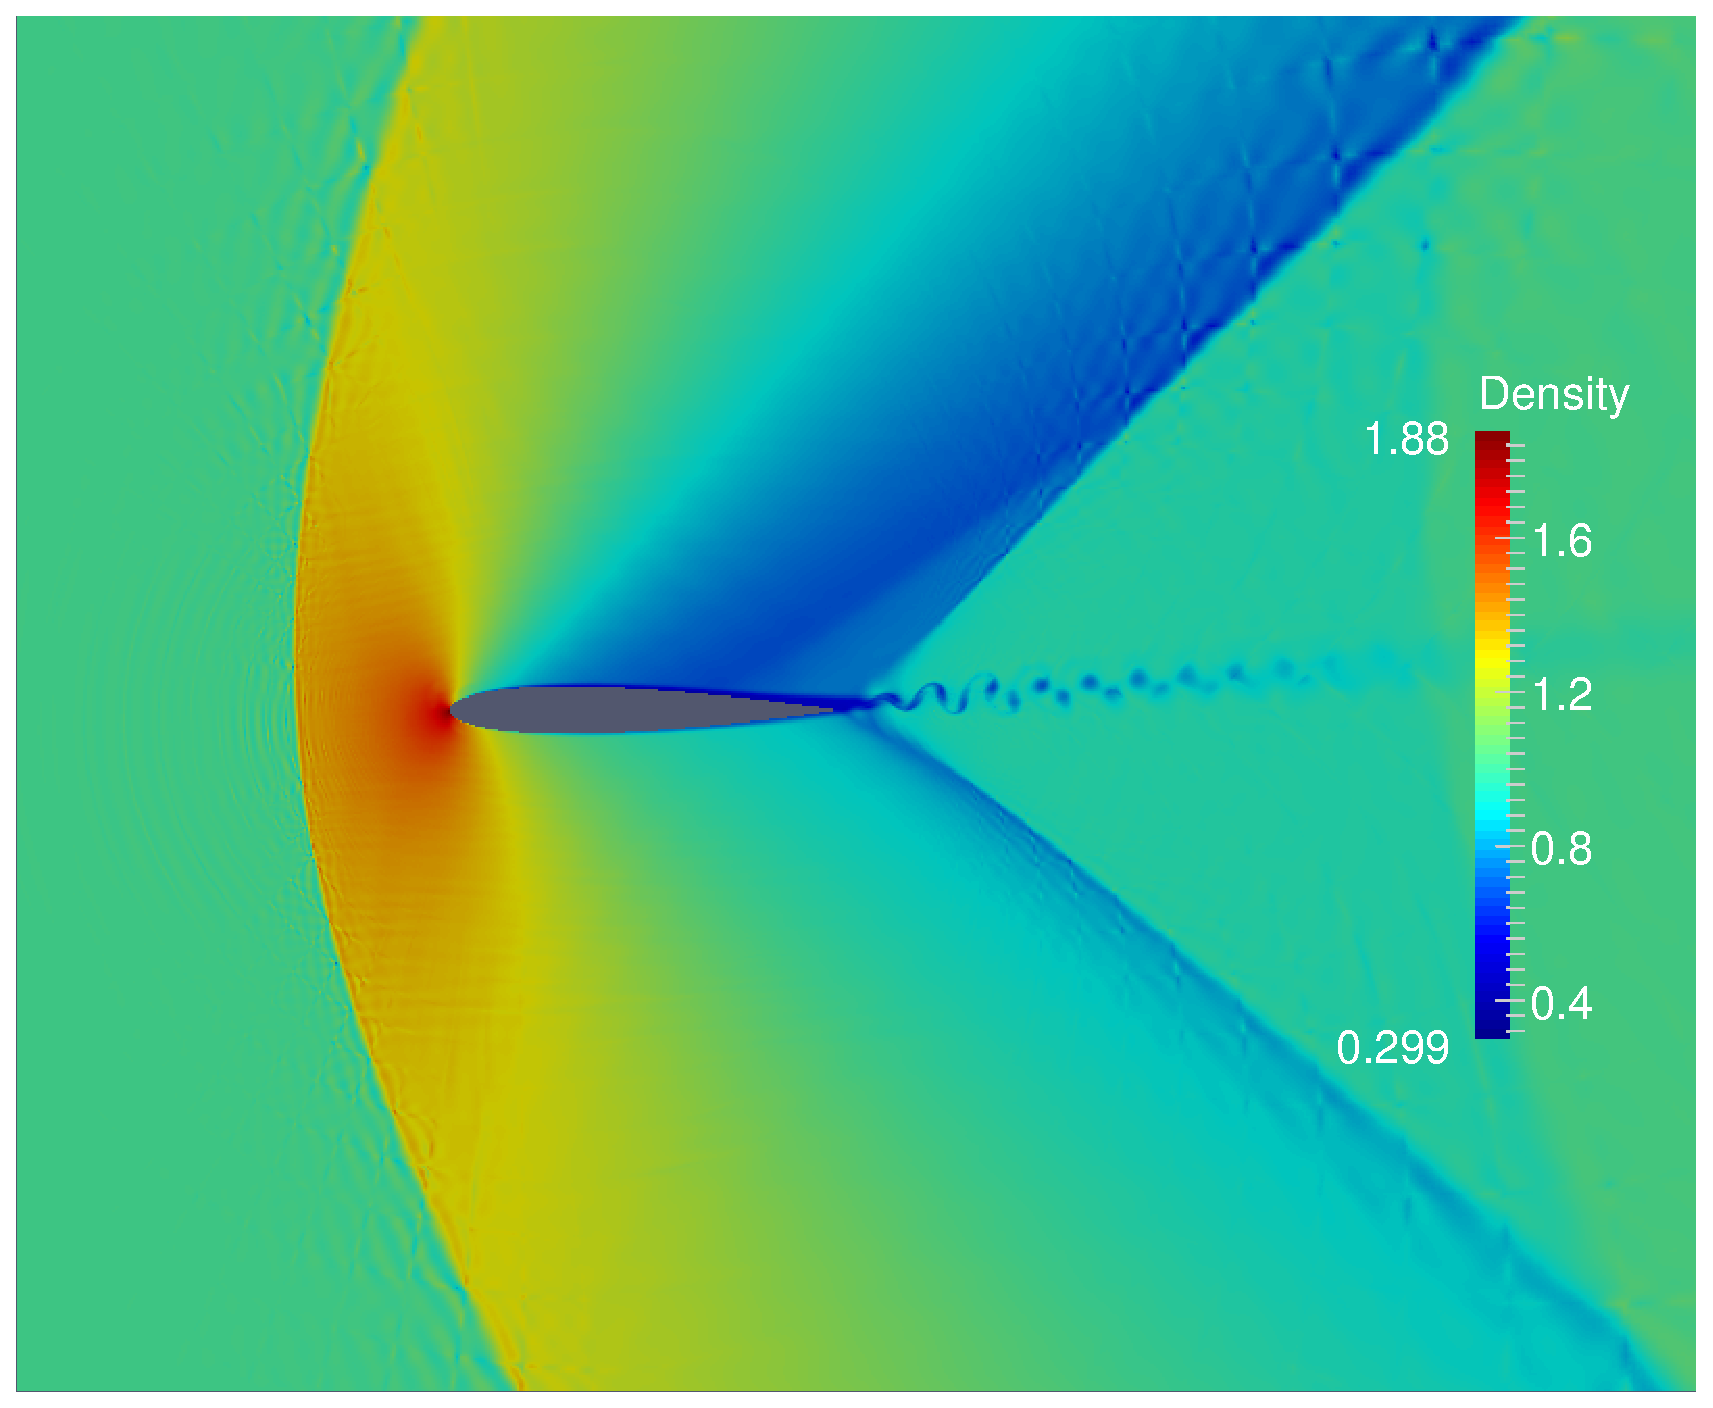
\includegraphics[width=.85\linewidth]{\aiaafigs /density-t1050010-jet.eps}
  \captionof{figure}{density contours for viscous flow at \gls{ma} = 1.2 over a NACA 0012 airfoil at 5$^{\circ}$ \gls{aoa} with polynomial order 6}
  \label{fig:visM1pt2-density}
\end{minipage}%
\begin{minipage}[t]{.5\textwidth}
  \centering
  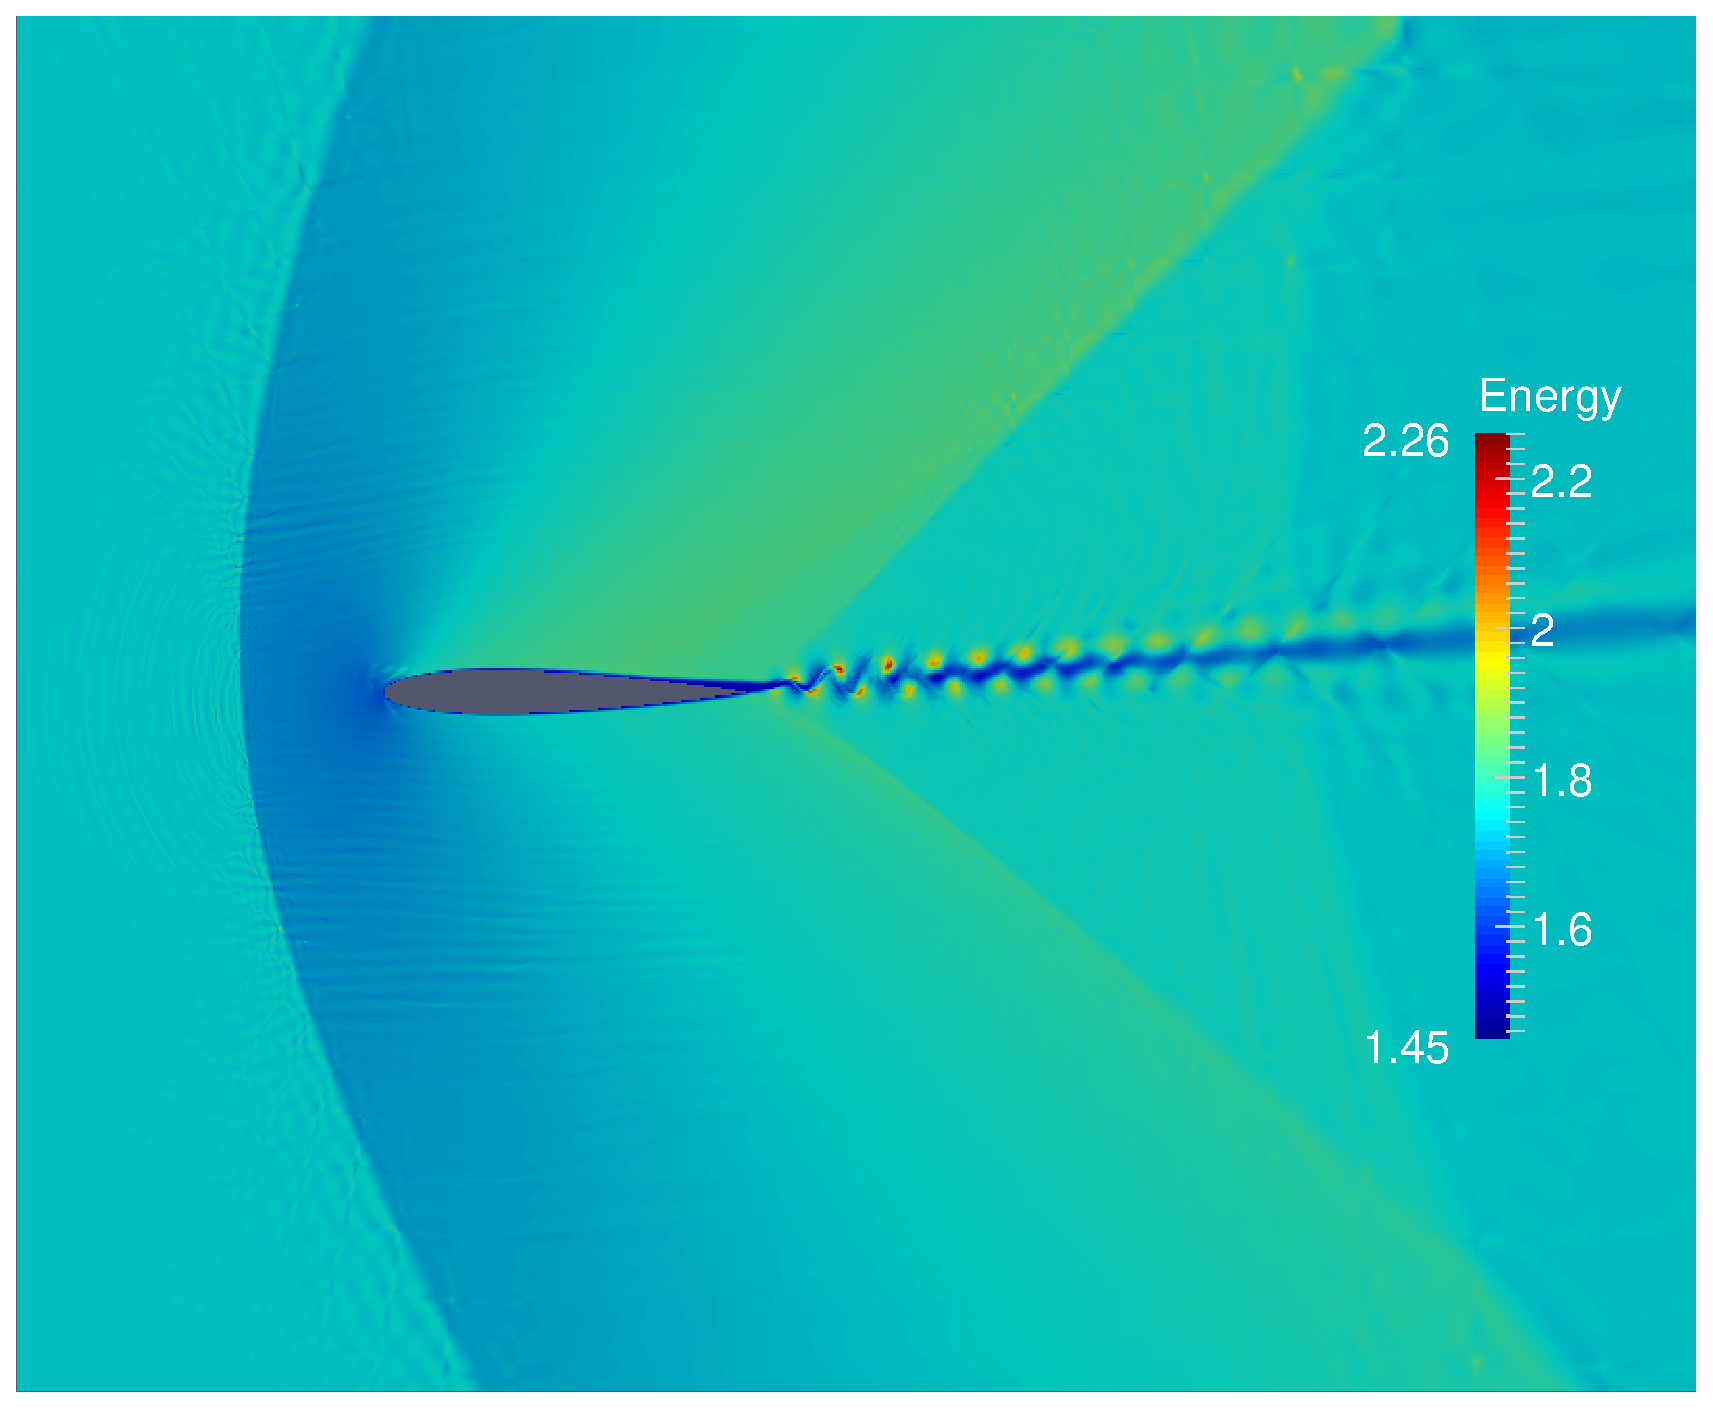
\includegraphics[width=.85\linewidth]{\aiaafigs /energy-t1050010-jet.eps}
  \captionof{figure}{Energy contours}
  \label{fig:visM1pt2-energy}
\end{minipage}
\end{figure} 

\begin{figure}[h] \tt
\centering
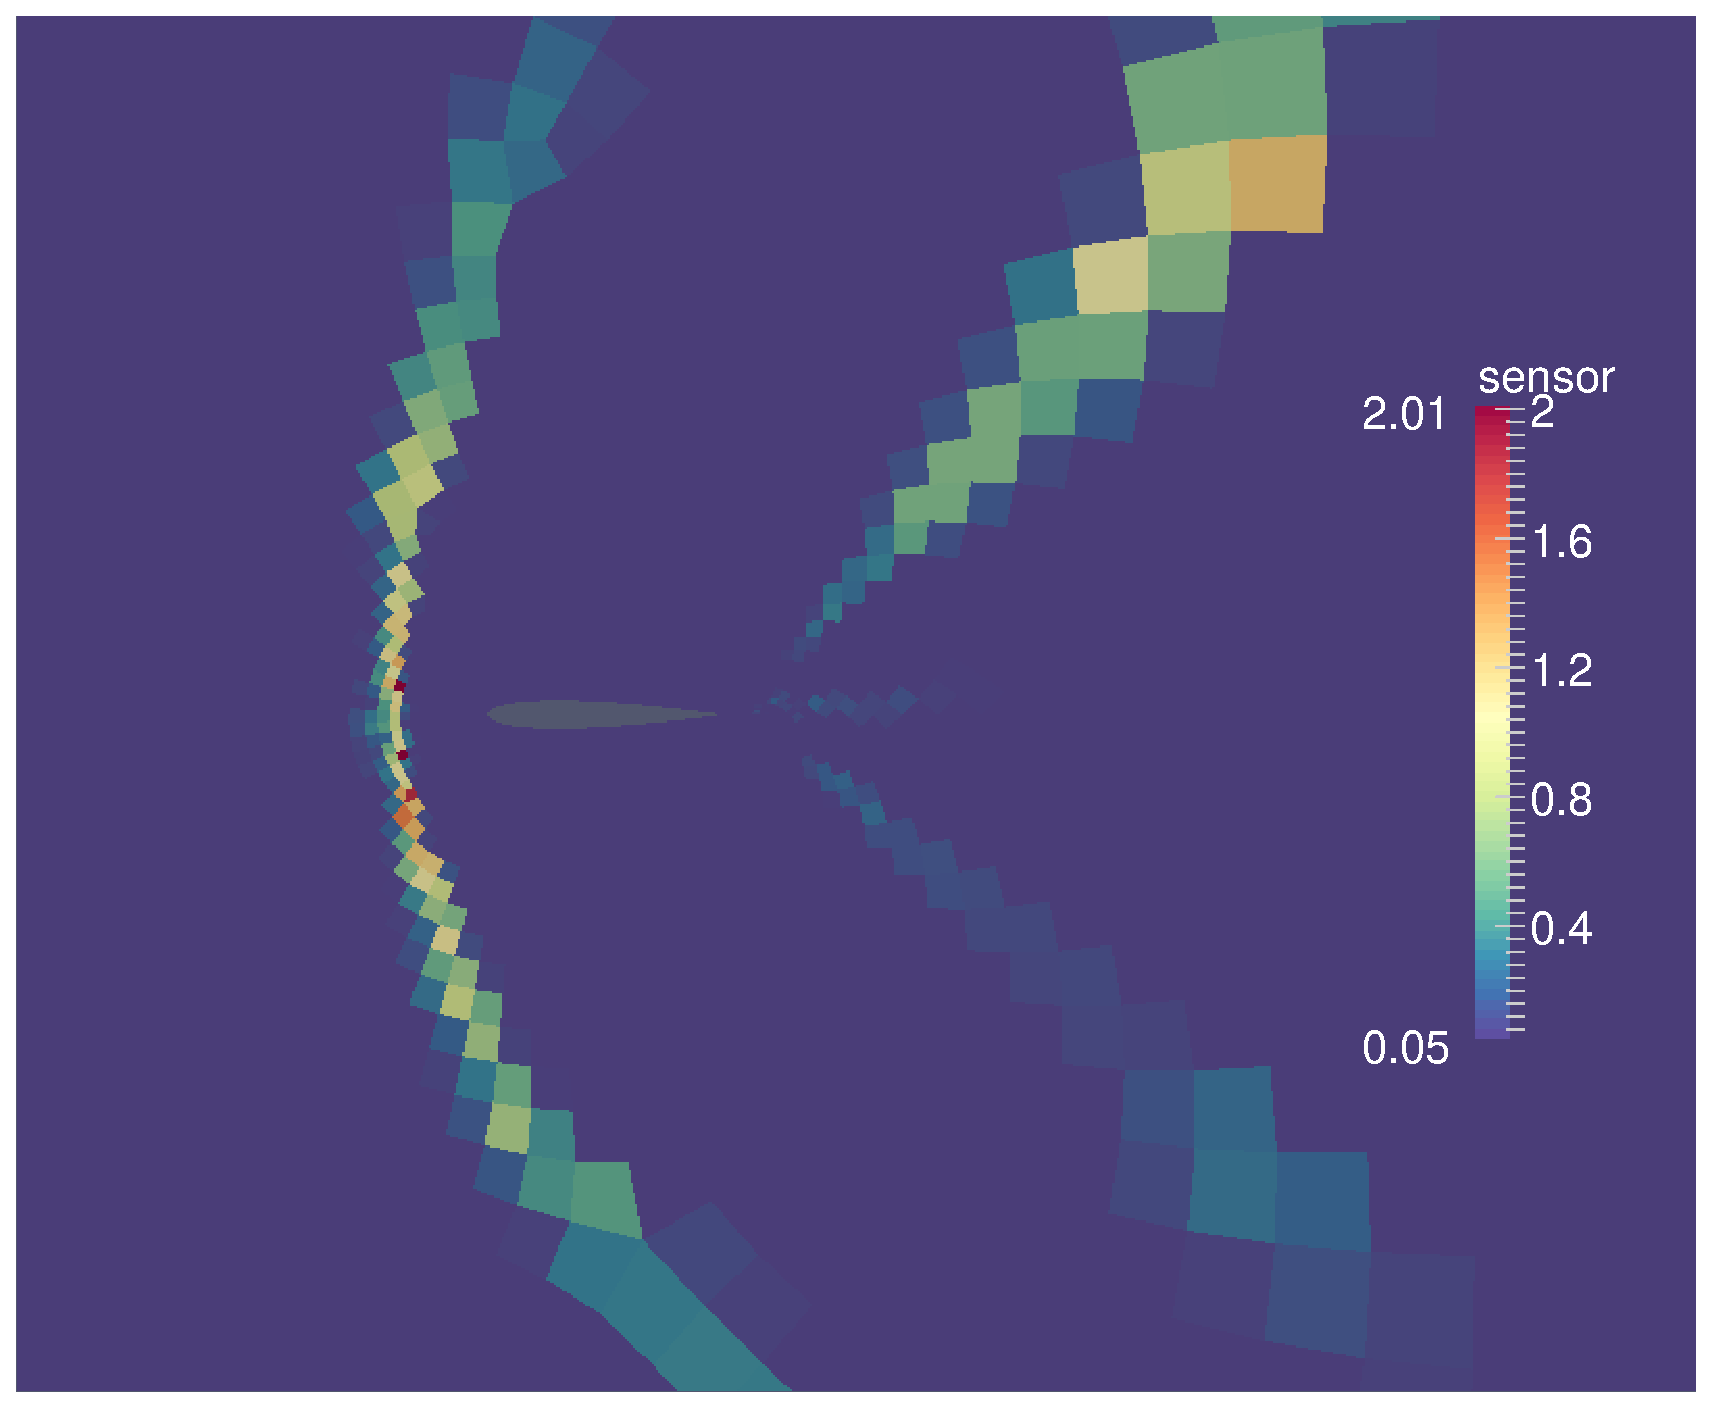
\includegraphics[width = 0.5\textwidth]{\aiaafigs /sensor-t1050010-spectral.eps}
\caption{Figure shows the elemental shock ``sensor'' for the \gls{ma} = 1.2 viscous case shown in figure ~\ref{fig:visM1pt2-density}. The shock sensor is just the maximum value of the enhanced kernel in each element}
\label{fig:sensor}
\end{figure}

\begin{figure}[h] \tt
\centering
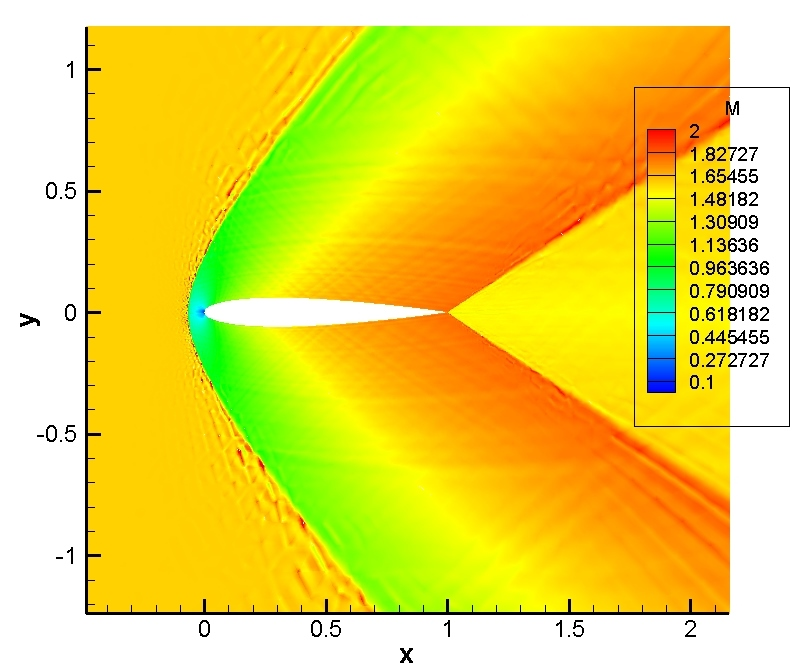
\includegraphics[width = 0.5\textwidth]{\aiaafigs /M1pt6order3-inv-720ktime-mach.jpg} \\
\caption{\gls{ma} contours for inviscid flow over NACA0012 at \gls{ma} = 1.6 and \gls{aoa} = $0^{\circ} $ on a triangle-mesh using Persson and Peraire's method and using artificial viscosity}
\label{fig:inv_mach}
\end{figure}

\begin{figure}
\centering
\begin{minipage}[t]{.55\textwidth}
  \centering
  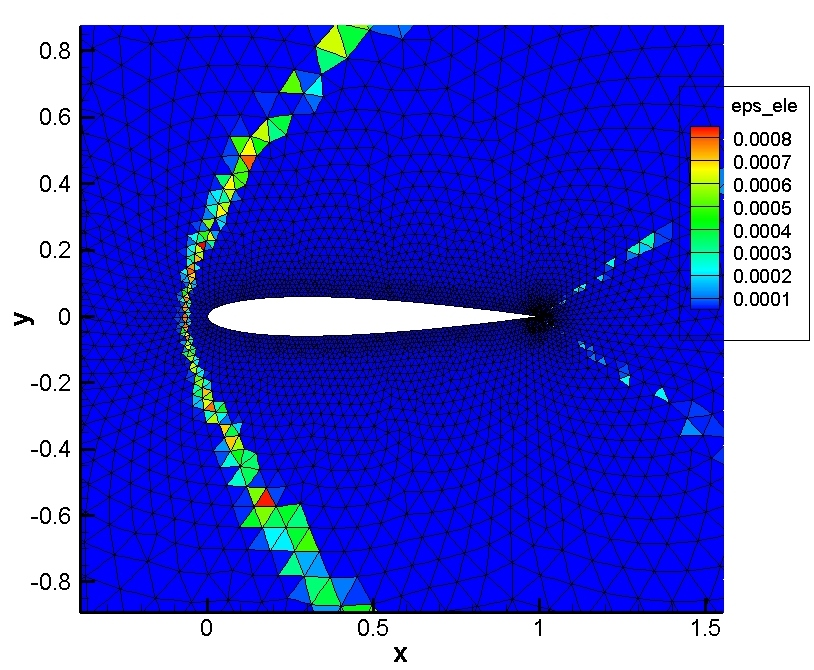
\includegraphics[width=.85\linewidth]{\aiaafigs /M1pt6-inv-av-ele-mesh}
  \caption{Element-wise \gls{av} coefficients for the inviscid \gls{ma}= 1.6 case}
  \label{fig:AV-ele}
\end{minipage}%
\begin{minipage}[t]{.55\textwidth}
  \centering
  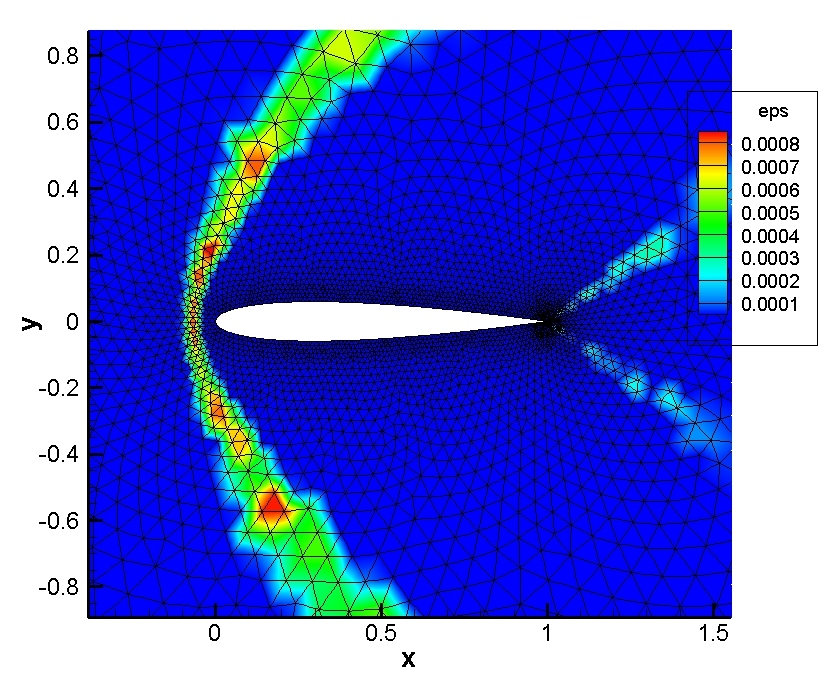
\includegraphics[width=.85\linewidth]{\aiaafigs /M1pt6-inv-av-mesh}
  \caption{\gls{av} coefficients with continuity enforcement}
  \label{fig:AV-cont}
\end{minipage}
\end{figure} 

\subsection{\gls{sa} Turbulence Model and Negative $\tilde\nu$ Modification}

The one equation \gls{sa} turbulence model is one of the more commonly used turbulence models used to solve attached and moderately separated aerodynamic flows~\cite{spalart1992one}. The added equation directly solves for turbulent eddy viscosity via advection, diffusion, production and dissipation. A modified form of the equation can be written as \cite{burgess2012robust,oliver2008high,moro2011navier}:
\begin{equation}
\begin{split}
	\frac{\partial}{\partial t}(\rho\tilde\nu) + \nabla\cdot(\rho\tilde\nu\boldsymbol{u}) = c_{b_1}\tilde S \rho\nu\psi &+ \frac{1}{\sigma}\left[\nabla\cdot((\mu + \mu\psi)\nabla\tilde\nu) + c_{b_2}\rho\nabla\tilde\nu\cdot\nabla\tilde\nu\right] \\&- c_{w_1}\rho f_w \left(\frac{\nu\psi}{d}\right)^2
\end{split}
\end{equation}

where $\tilde\nu$ is a modified version of the kinematic eddy viscosity and $\nu$ is the kinematic viscosity. The other variables are defined as:

\begin{align}
	 \mu_t =
	  \begin{cases}
	   \rho\tilde\nu f_{v_1} & \text{if } \tilde\nu \ge 0 \\
	   0       & \text{if } \tilde\nu < 0
	  \end{cases}
	  \quad \mbox{where} \quad f_{v_1} = \frac{\left(\frac{\rho\tilde\nu}{\mu}\right)^3}{\left(\frac{\rho\tilde\nu}{\mu}\right)^3 + c_{v_1}^3}
\end{align}

\begin{align}
	\tilde S &=
	\begin{cases}
	   S + \bar S & \text{if } \bar S \ge -c_{v_2}S \\
	   S + \frac{S(c_{v_2}^2 S + c_{v_3}\bar S)}{(c_{v_3} - 2c_{v_2})S - \bar S} & \text{if } \bar S \le -c_{v_2}S
	\end{cases}
\end{align}
\begin{align}
	S &= \sqrt{\boldsymbol{\omega}\cdot\boldsymbol{\omega}}
	\qquad \bar S = \frac{(\nu\psi)^2 f_{v_2}}{\kappa^2 d^2} \\
	f_{v_2} &= 1 - \frac{\psi}{1 + \psi f_{v_1}}
\end{align}

\begin{align}
	f_w &= g\left[\frac{1 + c_{w_3}^6}{g^6 + c_{w_3}^6}\right]^{1/6} 
	\qquad g = r + c_{w_2}(r^6 - r) 
	\qquad r = \frac{\nu\psi}{\tilde S \kappa^2 d^2}
\end{align}

where S is the magnitude of vorticity, d is the closest distance to a wall, $c_{b1} = 0.1355$, $\sigma = \frac{2}{3}$, $c_{b2} = 0.622$, $K = 0.41$, $\text{Pr}_t = 0.9$, $c_{v1} = 7.1$, $c_{v2} = 0.7$, $c_{v3} = 0.9$, $c_{w1} = \frac{c_{b1}}{K^2} + \frac{(1+c_{b2})}{\sigma}$, $c_{w2} = 0.3$, $c_{w3} = 2$.\\

The diffusion term, $\nabla\cdot(\rho\tilde\nu\boldsymbol{u})$, may become discontinuous in the first derivative leading to oscillations in high-order polynomials. This can lead to large negative values of the modified eddy viscosity term, $\tilde\nu$, significant enough to cause an unbounded solution. To prevent this, the following modification is introduced \cite{moro2011navier}.
\begin{align}
	\psi &=
	\begin{cases}
	   0.05log(1.0 + e^{(20.0\chi)}) & \text{if } \chi \le 10.0, \\
	   \chi & \text{if } \chi > 10.0,
	\end{cases} \\
	\chi &= \frac{\tilde\nu}{\nu}
\end{align}

\subsection{Large Eddy Simulation}\label{lesmodels}

In order to resolve all the scales of motion in a high \gls{re} number turbulent flow, the computational mesh would have to be exceedingly fine.
A practical solution is to employ the \gls{les} formulation, which only resolves the larger scales of motion and thus allows for the use of coarser meshes.

The effect of the unresolved or \gls{sgs} dynamics on the solution is accounted for by an \gls{sgs} model for the subgrid-scale stress $\tau_{ij}$, which is added to the viscous stress tensor $\sigma_{ij}$ given by (\ref{sigma}):

\begin{eqnarray}\label{tausgs}
\sigma_{ij} &&= 2 \mu S^d_{ij} + \tau_{ij},\\
S^d_{ij} &&= \frac 1 2 \l( \frac{\partial u_i}{\partial x_j} + \frac{\partial u_j}{\partial x_i} - \frac{2}{3} \delta_{ij}\frac{\partial u_k}{\partial x_k} \r).
\end{eqnarray}

The standard Smagorinsky model~\cite{smagorinsky1963} is available in \gls{hf}:
\begin{eqnarray}\label{smag}
\tau_{ij} &&= 2 \mu_t S^d_{ij}, \\
\mu_t &&= \rho C_S^2 \bigtriangleup^2 | S^d |,\\
| S^d | &&= \sqrt{2 S^d_{ij} S^d_{ij}},
\end{eqnarray}
where $\mu_t$ is the eddy viscosity, $C_S = 0.1$ is the Smagorinsky coefficient and $\bigtriangleup$ is the filter width. In \gls{hf} the filter width is given by (in 3D):
\begin{equation}
\bigtriangleup = \alpha (\text{vol})^{1/3},
\end{equation}
where $\alpha \geq 1$ is a user-defined scaling factor and vol is the element volume.

\gls{hf} also includes the \gls{wale} model~\cite{nicoud1999} and the Similarity model~\cite{bardina1980}.
The Similarity model incorporates a low-pass filtering operator, for which several choices are available in \gls{hf}: a discrete Gaussian filter\cite{lodato2012b}, a high-order commuting Vasilyev-type filter\cite{vasilyev1998,vasilyev2001} and a modal Vandermonde-type filter\cite{blackburn2003}.

The modal filter can be used on unstructured tetrahedral meshes. For details of these operators, see Lodato, Castonguay and Jameson~\cite{lodato2012b} and Bull and Jameson~\cite{bull2014a}. One can combine the similarity model with the Smagorinsky or \gls{wale} model to form a mixed \gls{sgs} model. The \gls{wsm} model, first proposed by Lodato et al.~\cite{lodato2009}, was used in simulations of the flow over a square cylinder (see Section~\ref{sqcyl}).

\subsection{Computing Architecture and Scalability}

The \gls{hf} code has been designed to work on multi-CPU as well as multi-CPU-\gls{gpu} platforms. The \gls{fr} method in its current form with explicit time-stepping has a great potential for parallelization. Since the solution points are not explicitly shared between elements, most of the computations are element-local enabling an efficient use of shared memory on \gls{gpu}s. Also, several computations are independent for each solution point and the highly parallelizable nature of \gls{gpu}s becomes very useful. A detailed description of the parallelization of the \gls{fr} method, along with scalability and performance analysis has been performed in~\cite{castonguay2011}.

% !TEX root = ../thesis.tex

\section{Verification and Validation}

\label{sec:verification}

% Manufactured solutions
% !TEX root = ../thesis.tex
\graphicspath{{figures_manufactured/}}% Set graphics path location


\subsection{Method of Manufactured Solutions}

This section describes the test of \gls{hf}'s spatial order of accuracy using the \gls{mms} in 2D and 3D for viscous flows. As shown by Salari et. al~\cite{salari2000code}, the \gls{mms} test rigorously assesses the correctness of implementation of a solver of \gls{pde}s. Simplex elements are crucial for simulations in unstructured meshes and have a more complex implementation than squares and hexahedra. As a result, we perform the \gls{mms} test in grids using simplex elements.

The \gls{mms} test for \gls{ns} solvers requires checking the solver's solution against an exact solution. Such exact solution can be chosen arbitrarily. The \gls{ns} equations can be satisfied with this arbitrary solution by including a time-dependent source term in the equations. Then, we solve

\begin{equation}
\frac{\partial U}{\partial t} +  \nabla \cdot {\bf F} = S
\end{equation}

For the following tests, we selected a smooth exact solution, so aliasing does not pollute the results. We picked

\begin{equation}\label{eq:NSwithSource}
\begin{split}
U_{2D} = \l(
\begin{tabular}{c}
$\sin{(k(x+y) - \omega t)} + a$\\
$\sin{(k(x+y) - \omega t)} + a$\\
$\sin{(k(x+y) - \omega t)} + a$\\
$(\sin{(k(x+y) - \omega t)} + a)^2$
\end{tabular}
\r) \\
U_{3D} = \l(
\begin{tabular}{c}
$\sin{(k(x+y+z) - \omega t)} + a$\\
$\sin{(k(x+y+z) - \omega t)} + a$\\
$\sin{(k(x+y+z) - \omega t)} + a$\\
$\sin{(k(x+y+z) - \omega t)} + a$\\
$(\sin{(k(x+y+z) - \omega t)} + a)^2$
\end{tabular}
\r)
\end{split}
\end{equation}

To find the value of $S$, we plug the values of our selected $U$ into the left-hand side of Equation~\eqref{eq:NSwithSource} and simplify. The resulting expression is $S$. 
We let \gls{pr}$=0.72, \gamma = 1.4, k = \pi, \omega = \pi, a = 3.0$ and $\mu = 0.001$.

The meshes used have dimensions $[-1,1] \times [-1,1]$ in 2D and $[-1,1] \times [-1,1] \times [-1,1]$ in 3D. Periodic boundary conditions were applied on the boundaries of the square and cube domains. Uniform square and cubic meshes were created and then each element was subdivided into triangles or tetrahedra. Two triangles were created from each square, and six tetrahedra were created from each cube. Consequently, in 2D a $N \times N$ mesh contains $2N^2$ triangles, and in 3D a $N \times N \times N$ mesh contains $6N^3$ tetrahedra. 


In 3D, the time step was $1$e$-4$ seconds and 10 seconds of flow were simulated. In 2D, the time step was $1$e$-6$ seconds and 1 second of flow was simulated. The time-stepping scheme used was the low-storage, $4^\text{th}$ order accurate \gls{rk45} method. 


\input{\aiaadir /summaryTable_ele1_err1.tex}
\input{\aiaadir /summaryTable_ele1_err2.tex}
\input{\aiaadir /summaryTable_ele2_err1.tex}
\input{\aiaadir /summaryTable_ele2_err2.tex}

Tables \eqref{table:trisError1} and \eqref{table:tetsError1} show the spatial order of accuracy achieved when calculating the energy fields $\rho e$ in 2D and 3D, respectively. Tables \eqref{table:trisError2} and \eqref{table:tetsError2} show the order of accuracy for the gradient of the energy field $\frac{\partial }{\partial x_i}(\rho e)$ in 2D and 3D, respectively. Because of the exact solutions that were picked, the exact values of the gradients of $\rho e$ in the $x,y,z$ directions are equal.

As expected\cite{hesthaven2007nodal}, the order of accuracy of the solution is $p+1$ and the order of accuracy of the gradient of the solution is $p$, where $p$ is the order of the polynomial used to approximate the solution fields. In the fifth order simulations, the relatively large time step introduces errors larger than the spatial discretization errors. Hence we observe sub-optimal orders of convergence in the coarsest meshes.

%\begin{figure}
%\centering
%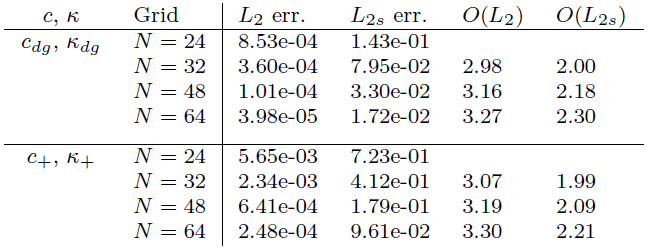
\includegraphics[height=35mm]{table_917} \\
%\caption{Accuracy of ESFR schemes for flow generated by a time-dependent source term on triangular grids, for the case of $p = 2$. The inviscid and viscous numerical fluxes were computed using a Rusanov flux with $\lambda = 1$ and a LDG flux with $\tau = 0.1$ and $\beta = \pm 0.5n$.}
%\label{fig:table_917}
%\end{figure}
%
%\begin{figure}
%\centering
%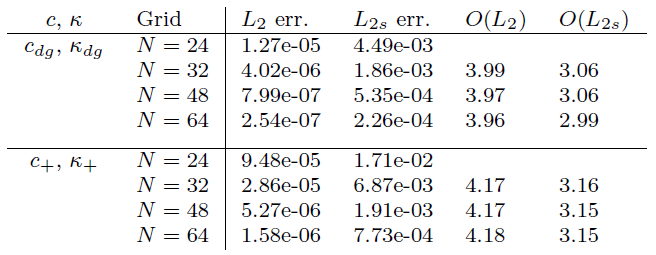
\includegraphics[height=35mm]{table_918} \\
%\caption{Accuracy of ESFR schemes for flow generated by a time-dependent source term on triangular grids, for the case of $p = 3$. The inviscid and viscous numerical fluxes were computed using a Rusanov flux with $\lambda = 1$ and a LDG flux with $\tau = 0.1$ and $\beta = \pm 0.5n$.}
%\label{fig:table_918}
%\end{figure}
%
%\begin{figure}
%\centering
%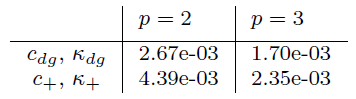
\includegraphics[height=20mm]{table_919} \\
%\caption{Explicit time-step limits ($\Delta t_{max}$) of ESFR schemes for flow generated by a time-dependent source term on the triangular grid with $\tilde{N} = 48$, for the cases of $p = 2$ and $3$. The inviscid and viscous numerical fluxes were computed using a Rusanov flux with $\lambda = 1$ and a LDG flux with $\tau = 0.1$ and $\beta = \pm 0.5n$.}
%\label{fig:table_919}
%\end{figure}
%
%\begin{figure}
%\centering
%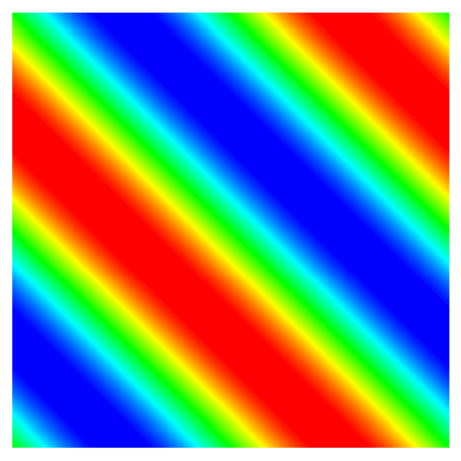
\includegraphics[height=60mm]{figure_912} \\
%\caption{Contours of energy obtained using the ESFR scheme with $c = c_+$ and $\kappa = \kappa_+$ on the triangular grid with $\tilde{N} = 32$ for the case of $p = 3$. The inviscid and viscous numerical fluxes were computed using a Rusanov flux with $\lambda = 1$ and a LDG flux with $\tau = 0.1$ and $\beta = \pm 0.5n$.}
%\label{fig:figure_912}
%\end{figure}
%
%\begin{figure}
%\centering
%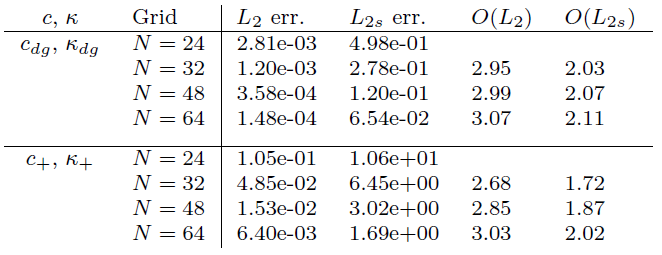
\includegraphics[height=35mm]{table_920} \\
%\caption{Accuracy of ESFR schemes for flow generated by a time-dependent source term on tetrahedral grids, for the case of $p = 2$. The inviscid and viscous numerical fluxes were computed using a Rusanov flux with $\lambda = 1$ and a LDG flux with $\tau = 0.1$ and $\beta = \pm 0.5n$.}
%\label{fig:table_920}
%\end{figure}
%
%\begin{figure}
%\centering
%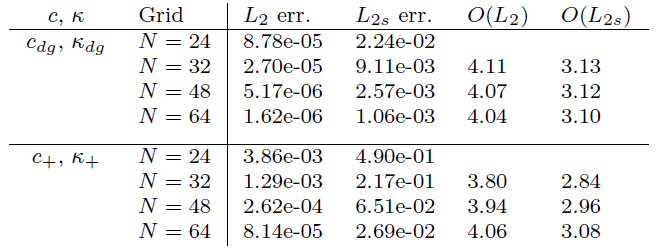
\includegraphics[height=30mm]{table_921} \\
%\caption{Accuracy of ESFR schemes for flow generated by a time-dependent source term on tetrahedral grids, for the case of $p = 3$. The inviscid and viscous numerical fluxes were computed using a Rusanov flux with $\lambda = 1$ and a LDG flux with $\tau = 0.1$ and $\beta = \pm 0.5n$.}
%\label{fig:table_921}
%\end{figure}
%
%\begin{figure}
%\centering
%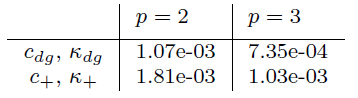
\includegraphics[height=15mm]{table_922} \\
%\caption{Explicit time-step limits ($\Delta t_{max}$) of ESFR schemes for flow generated by a time-dependent source term on the triangular grid with $\tilde{N} = 48$, for the cases of $p = 2 and 3$. The inviscid and viscous numerical fluxes were computed using a Rusanov flux with $\lambda = 1$ and a LDG flux with $\tau = 0.1$ and $\beta = \pm 0.5n$.}
%\label{fig:table_922}
%\end{figure}
%
%\newpage
%\begin{figure}
%\centering
%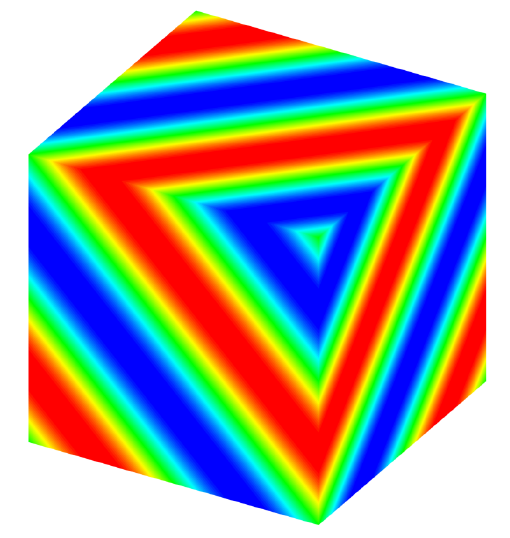
\includegraphics[height=60mm]{figure_913} \\
%\caption{Contours of energy obtained using the ESFR scheme with $c = c_+$ and $\kappa = \kappa_+$ on the tetrahedral grid with $\tilde{N} = 32$ for the case of $p = 3$. The inviscid and viscous numerical fluxes were computed using a Rusanov flux with $\lambda = 1$ and a LDG flux with $\tau = 0.1$ and $\beta = \pm 0.5n$.}
%\label{fig:figure_913}
%\end{figure}


% Flat plate
% !TEX root = ../thesis.tex
\graphicspath{{\aiaadir /figures_flatplate/}}% Set graphics path location

\subsection{Subsonic laminar flat-plate}

Computations of the flow over a subsonic flat-plate have been performed and validated against the Blasius' solution for laminar boundary layer. The flow conditions are \gls{ma} $0.5$, 0$\degr$ angle of attack and \gls{re} $1\cdot10^6$ based on the plate length. The governing equations are the 2D \gls{ns} equations with constant ratio of specific heats of $1.4$, Prandtl number of $0.72$ and constant dynamic viscosity of $1.827\cdot 10^{-5} Pa \cdot s$.

\begin{center} 
    \begin{tabular}{l*{7}{c}r}
    Mesh & First cell height & \specialcell{\# of cells in \vspace{0.2cm}\\boundary layer} & $p_3$ & $p_4$ & $p_5$ & $p_6$ \\ \hline
    Mesh a0 (140 = 14x10) & 0.00075 & 2 & $\times$ & $\times$ & $\times$ & \Checkmark \\ \hline
    Mesh a1 (560 = 28x20) & 0.000375 & 4 &  $\times$ & $\times$ & \Checkmark & \Checkmark \\ \hline
    Mesh a2 (2240 = 56x40) & 0.0001875 & 8 & $\times$ & \Checkmark & \Checkmark & \Checkmark \\ \hline
    Mesh a3 (8960 = 112x80) & 0.0000935 & 16 & \Checkmark & \Checkmark & \Checkmark & \Checkmark \\
    \hline
    \end{tabular} 
      \captionof{table}{\gls{hf} convergence using different grids and polynomial order. $\times$ / \Checkmark indicates not converged/converged resp.} \label{tab:convergence} 
\end{center}

The objective of this study is to determine the minimum number of elements and the order of polynomial required to converge the flat-plate simulation using \gls{hf}. Four different numerical grids have been used in this study (2, 4, 8, 16 elements inside the boundary layer) and four polynomial orders ($p_3$--$p_6$). The results, summarized in Table \ref{tab:convergence}, show that a minimum number of elements is needed in the boundary layer depending on the polynomial order to obtain satisfactory convergence (free from inter-element jumps).

\begin{figure}
\begin{center}
\begin{minipage}[t]{0.48\columnwidth}
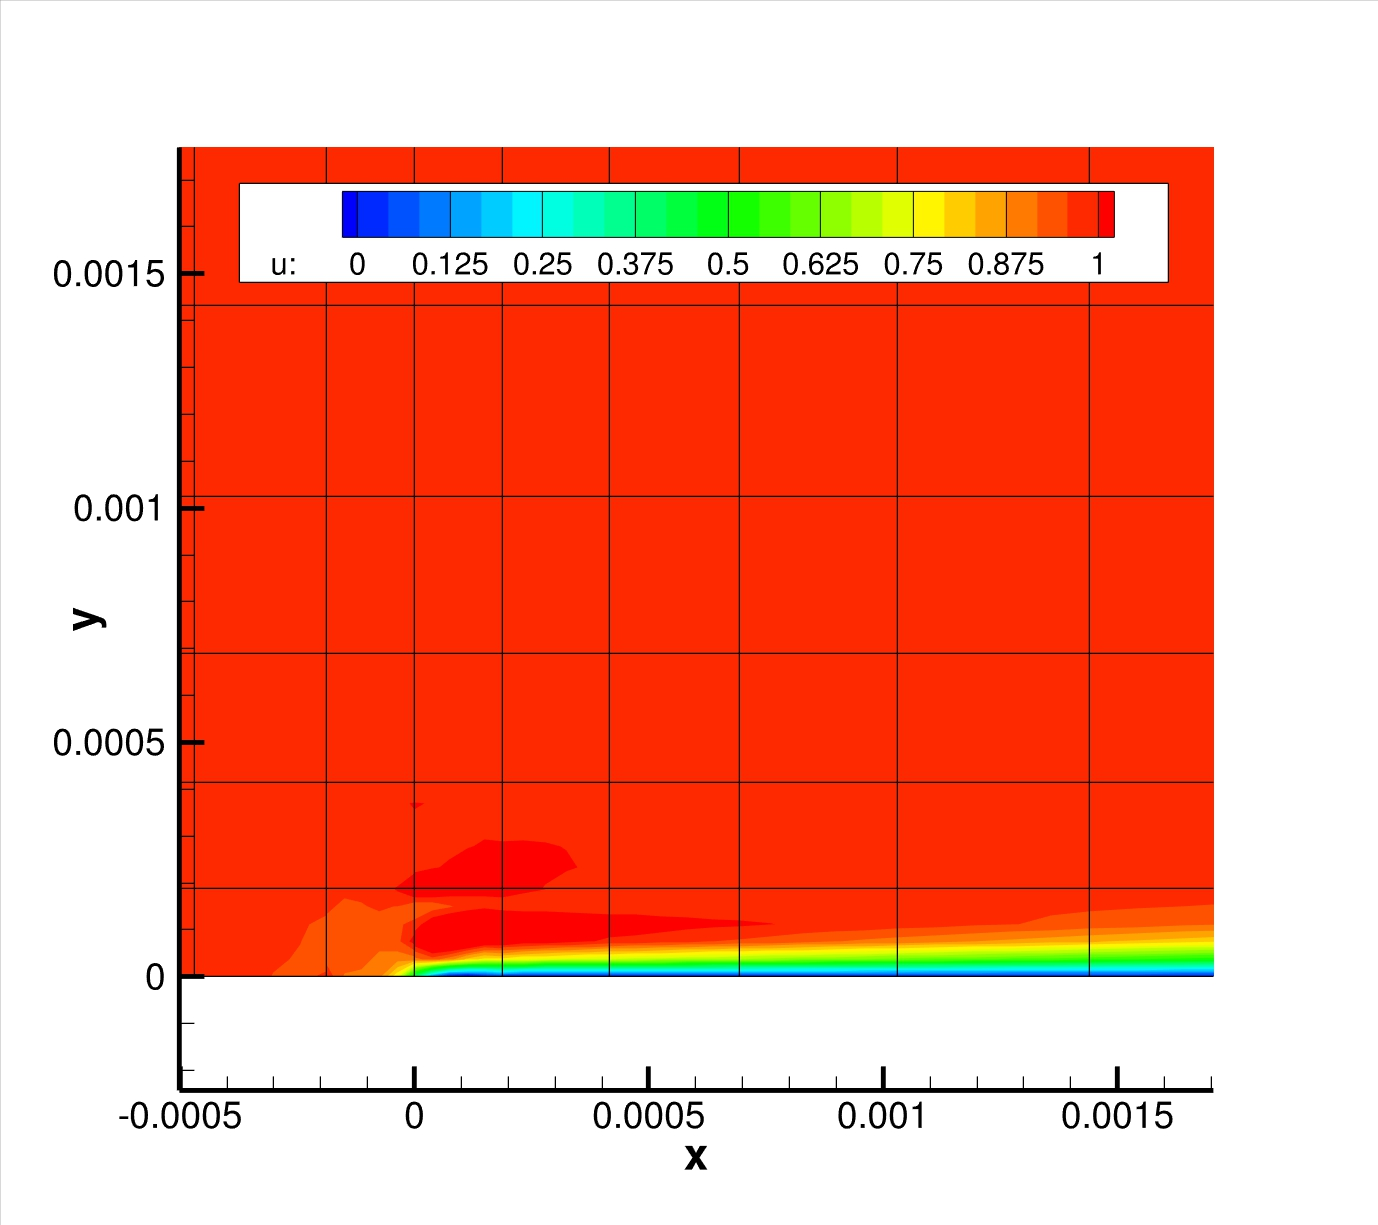
\includegraphics[width = \textwidth,clip=]{LeadingEdge.jpg}
\caption{Detail of the flat-plate leading edge (x=0.0, mesh a2).}
\label{fig:LeagingEdge}
\end{minipage}
\hfill
\begin{minipage}[t]{0.48\columnwidth}
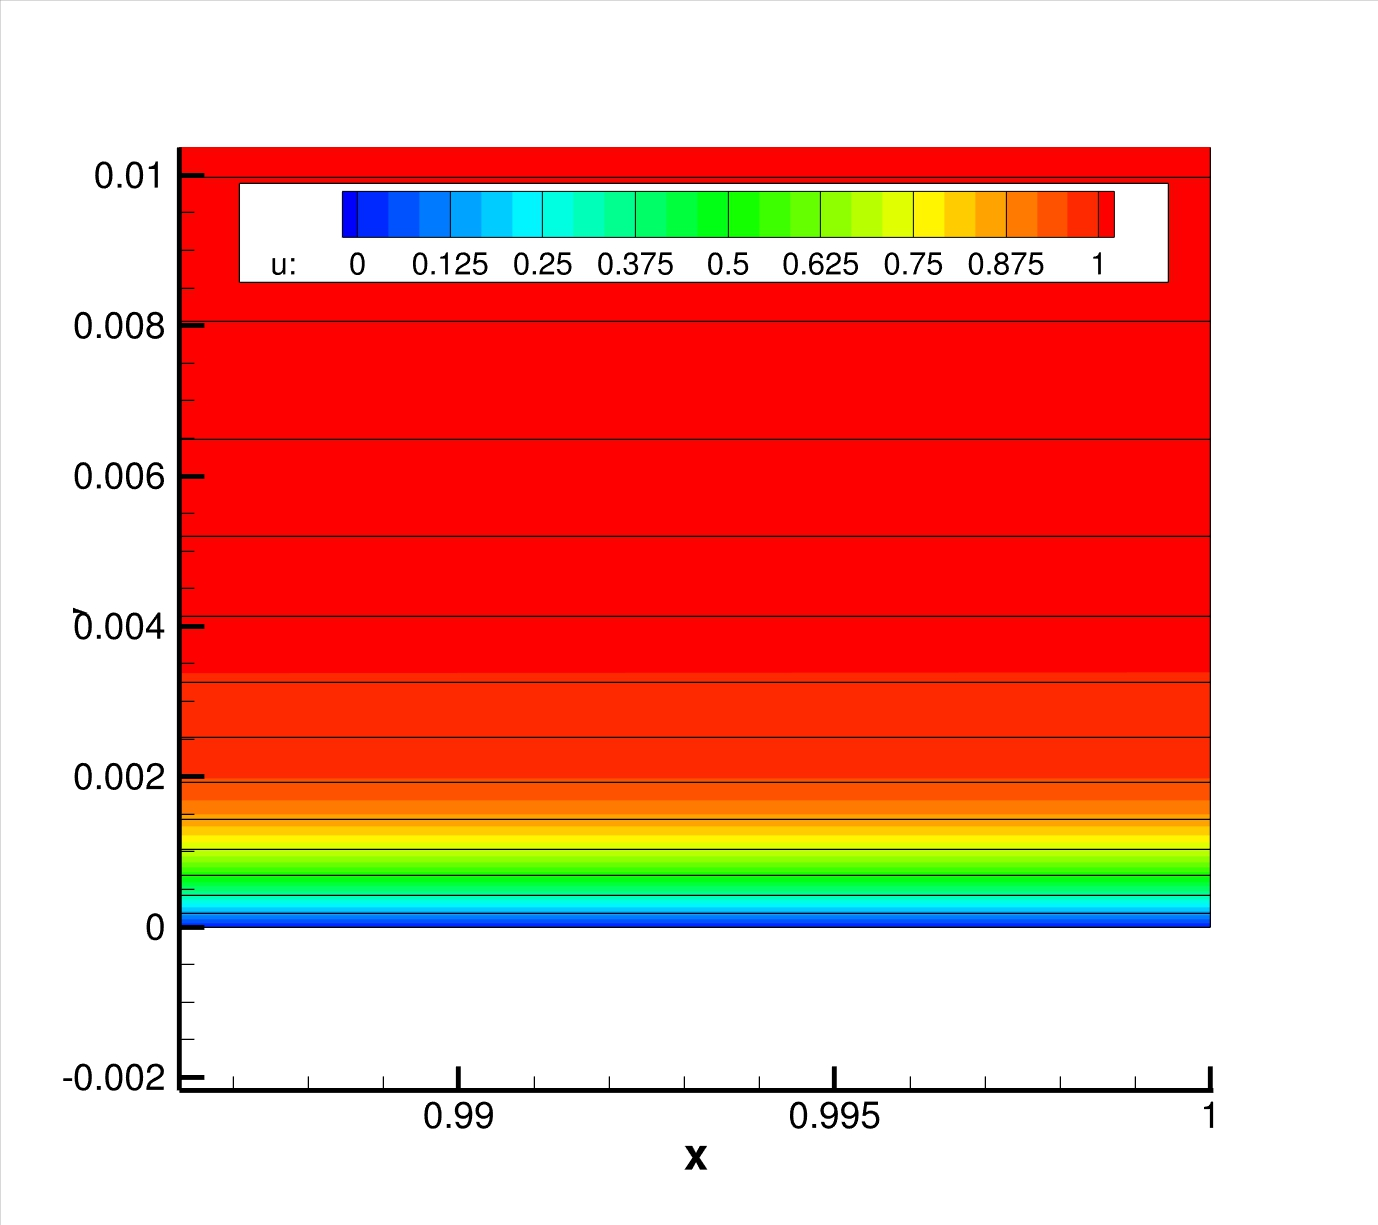
\includegraphics[width = \textwidth,clip=] {EndPlate.jpg}
\caption{Flow solution at the end of the flat-plate (x=1.0, mesh a2).}
\label{fig:TrailingEdge}
\end{minipage}
\end{center}
\end{figure}

The results are compared with the Blasius' solution for laminar boundary layer with satisfactory results, and some details of the solutions are presented in Fig. \ref{fig:LeagingEdge} (leading edge), and Fig. \ref{fig:TrailingEdge} (end of the flat-plate). It is important to note that in this particular case (mesh a2) the flat-plate boundary layer is captured using 8 elements, while in a second order solver it would be necessary of the order of ~30 elements inside the boundary layer.

\begin{figure}
\begin{center}
\begin{minipage}[t]{0.48\columnwidth}
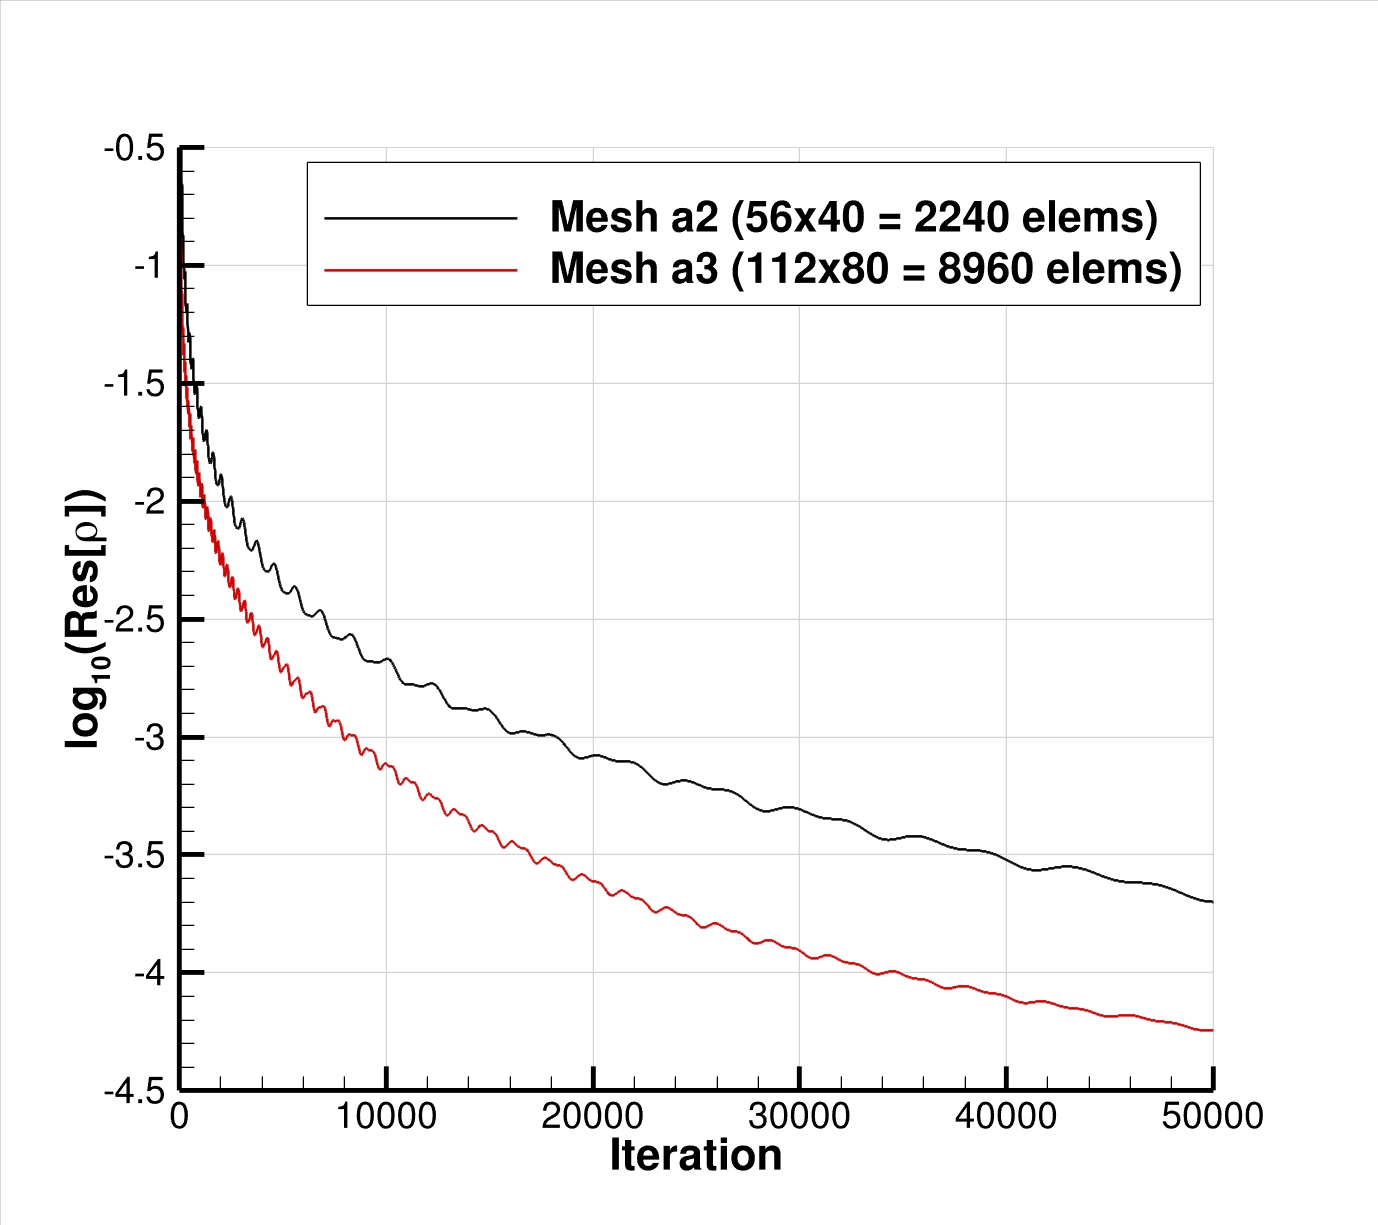
\includegraphics[width = \textwidth]{CompMesh.jpg}
\caption{Convergence comparison (3$^{rd}$ order, finest grids).}
\label{fig:ComparisonOrder}
\end{minipage}
\hfill
\begin{minipage}[t]{0.48\columnwidth}
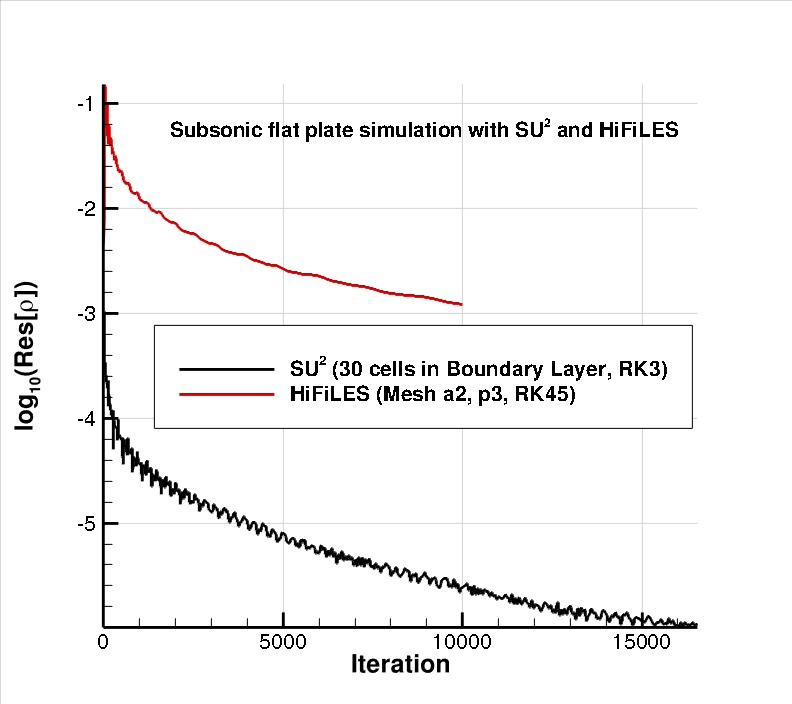
\includegraphics[width = \textwidth] {CompSu2.jpg}
\caption{Comparison of \gls{hf} with SU2 using a similar time integration scheme.}
\label{fig:Comparison_SecondOrder}
\end{minipage}
\end{center}
\end{figure}

To finalize, it is critical to note that the absence of a local time stepping technique in \gls{hf} increases the required number of iterations to obtain a converged solution. However, we have noticed an improvement of the rate of convergence as we refine the grid (see Fig. \ref{fig:ComparisonOrder}). The obtained convergence rate is comparable to a second order numerical code (e.g. SU2~\cite{palacios2013stanford,palacios14}) running using a similar numerical time integration (see Fig.~\ref{fig:Comparison_SecondOrder}).


% Circular cylinder
% !TEX root = ../thesis.tex
\graphicspath{{\aiaadir /figures_cylinder/}}% Set graphics path location

\subsection{Circular Cylinder}

The classic test case of laminar flow past a circular cylinder at low \gls{re} number has also been chosen as a verification and validation case for the 2D \gls{ns} equations in \gls{hf}, and the results are compared to existing experimental data and simulation results~\cite{park1998}. Two separate cases are computed: first, the steady flow past the cylinder at \gls{re}$= 20$, and second, the unsteady flow past the cylinder at \gls{re}$= 100$, where \gls{re} is based upon the diameter of the cylinder. For both cases, \gls{ma} number is set to 0.1 in order to recover nearly incompressible flow for comparisons with the existing incompressible results. The remaining flow conditions are $0\degr$ angle of attack, a constant ratio of specific heats of $1.4$, a Prandtl number of $0.72$, a free-stream temperature of $300K$, and a free-stream dynamic viscosity of $1.853\cdot 10^{-5} Pa \cdot s$ (laminar viscosity varies according to Sutherland's law during the simulation).

The two simulations are performed with third order polynomials on a mesh with $4988$ total elements that contains quadrilateral elements near the body of the cylinder and triangular elements out to the far-field. There is a small refinement box immediately downstream of the cylinder to help resolve features in the wake. The rectangular far-field boundaries are located approximately 30 diameters away from the cylinder in the upstream, upward, and downward directions and 50 diameters away in the downstream direction. A view of the mesh near the cylinder surface is show in Fig.~\ref{cylinder_1}.

\begin{figure}

    \subfloat[Zoom view of the mesh near the cylinder.]{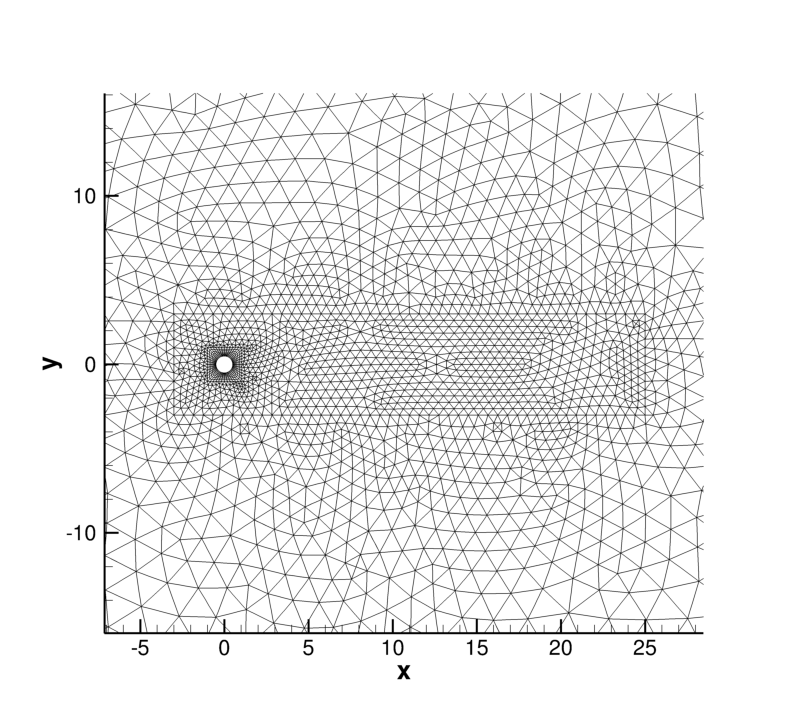
\includegraphics[width = 0.5\textwidth]{cylinder_mesh.png}}
    \subfloat[X-velocity contours and streamlines around the circular cylinder for $Re = 20$.]{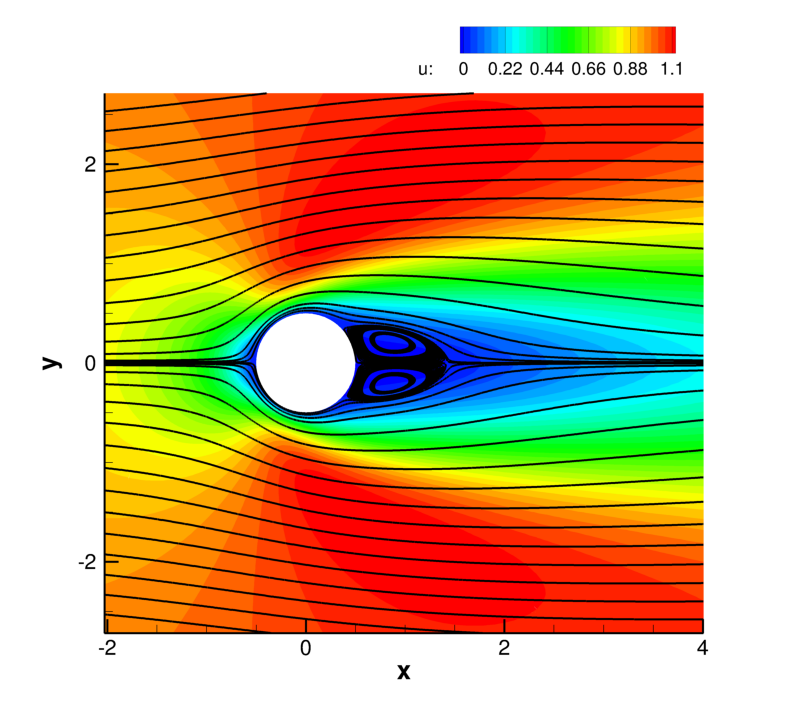
\includegraphics[width = 0.5\textwidth]{cylinder_streamlines.png}}
    
  \caption{The mesh for the circular cylinder simulations along with x-velocity contours for the $Re = 20$ case.}
  \label{cylinder_1}
\end{figure}

The flow around the cylinder for \gls{re}$= 20$ is steady, and it features a large recirculation region behind the cylinder. Fig.~\ref{cylinder_1} presents x-velocity contours around the cylinder along with streamlines. The length of the recirculation region can be determined from the streamlines, and a length of approximately one cylinder diameter agrees well with reported results for \gls{re}$= 20$. The coefficient of drag computed by \gls{hf} is $2.043$, which is close to the value of $2.01$ reported by Park et al.~\cite{park1998} Pressure contours around the cylinder are shown in Fig.~\ref{cylinder_2}.

\begin{figure}

    \subfloat[Pressure contours for the $Re = 20$ case.]{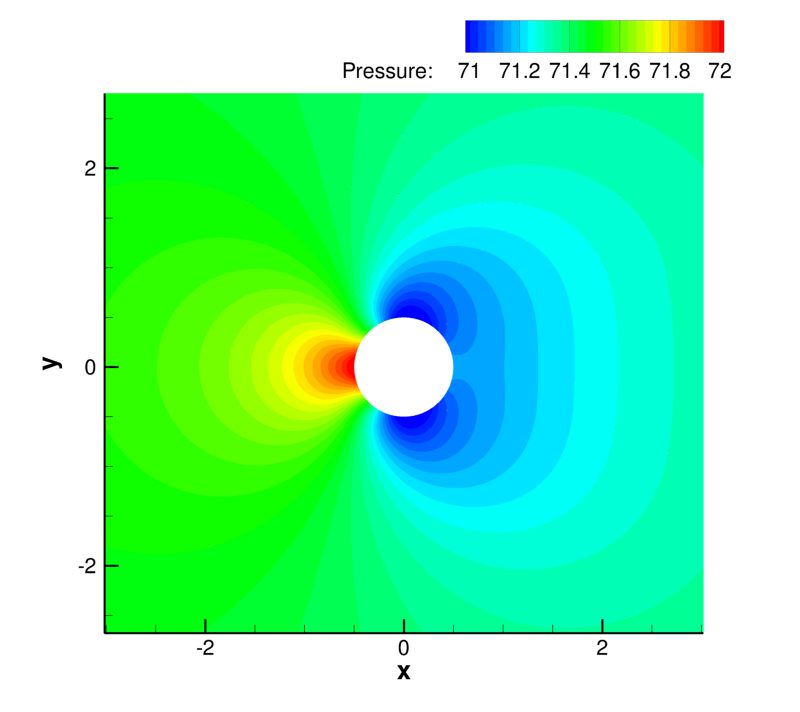
\includegraphics[width = 0.5\textwidth]{cylinder_pressure_re20.png}}
    \subfloat[Pressure contours for the $Re = 100$ case.]{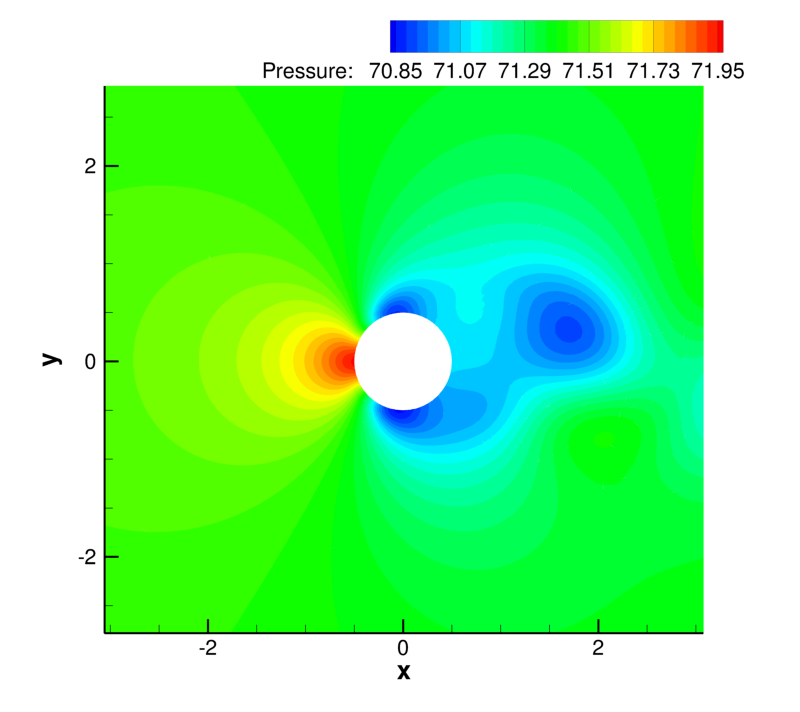
\includegraphics[width = 0.5\textwidth]{cylinder_pressure_re100.png}}

  \caption{Pressure contours for the steady and unsteady (instantaneous) cylinder cases.}
  \label{cylinder_2}
\end{figure}

When \gls{re} is increased to $100$, the flow around the cylinder becomes unsteady and exhibits periodic vortex shedding. This periodic shedding in the wake behind the cylinder can be seen in the instantaneous contours of x-velocity and vorticity in Fig.~\ref{cylinder_3}, and it also results in periodic fluctuations in the force coefficients on the cylinder. \gls{hf} reports an average drag coefficient of $1.339$ with a maximum deviation from this value of $0.0092$, which agree excellently with the values reported by Park et al.~\cite{park1998} of $1.33$ and $0.0091$ for the average $C_d$ and maximum deviation from it, respectively.  Instantaneous pressure contours for the \gls{re}$= 100$ case can be seen in Fig.~\ref{cylinder_2}. The asymmetry that is visible in the pressure contours contributes to the variability in the drag coefficient.

\begin{figure}
    \subfloat[X-velocity contours around the circular cylinder for \gls{re}$= 100$.]{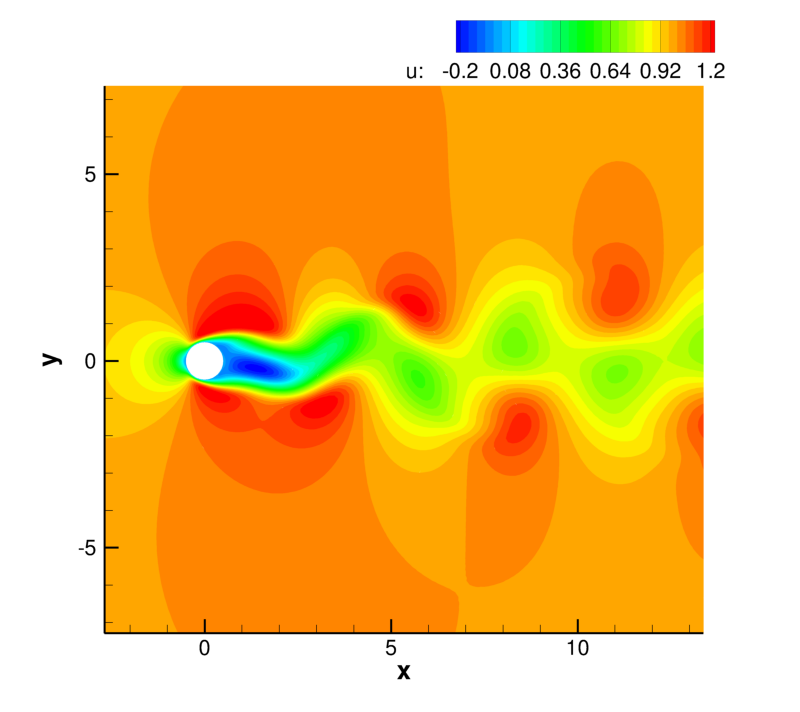
\includegraphics[width = 0.5\textwidth]{cylinder_xvelocity_re100.png}}
    \subfloat[Vorticity contours for the \gls{re}$= 100$ case.]{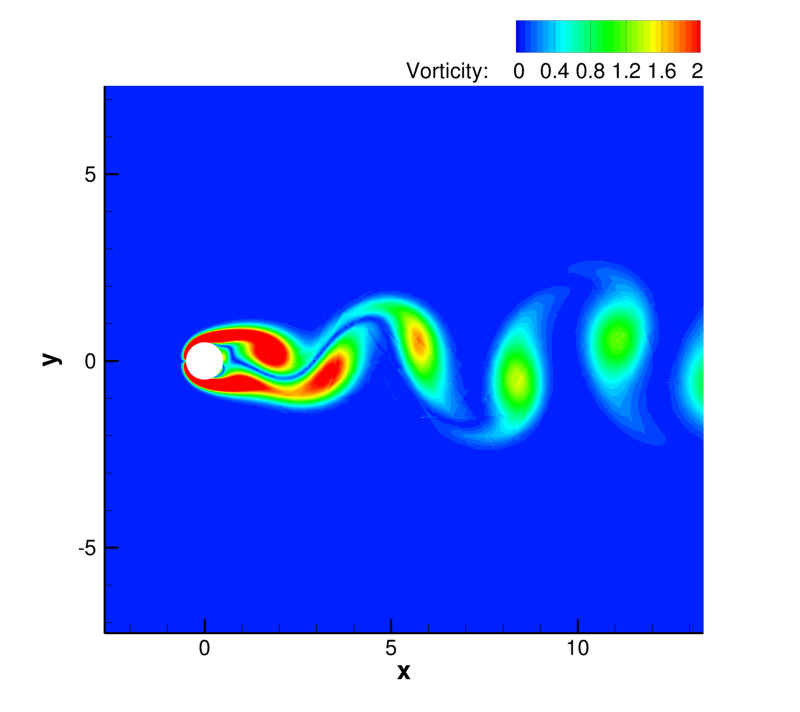
\includegraphics[width = 0.5\textwidth]{cylinder_vorticity_re100.png}}

  \caption{Instantaneous solution contours for the unsteady cylinder case.}
  \label{cylinder_3}
\end{figure}

% SD7003 section
% !TEX root = ../thesis.tex
\graphicspath{{\aiaadir /figures_SD7003/}}% Set graphics path location

\subsection{SD7003 airfoil at 4$\degr$ angle of attack}\label{sd7003airfoil}

Abundant literature documents flow around a SD7003 infinite wing and airfoil. Hence, physical experiments \cite{ol2005comparison,radespiel2007numerical} and numerical simulations \cite{galbraith2008implicit,visbal2009high,castonguay2010simulation,persson2011high,uranga2011implicit} of flow over this geometry can be used to benchmark \gls{hf}.

The simulations on the 2D geometry were performed on a circular domain with a radius of $50c$, where $c$ is the airfoil's cord length, centered at the leading edge of the airfoil. The boundary conditions are characteristic on the outer edge and adiabatic no-slip wall on the airfoil. The Mach number for all simulations was \gls{ma}$= 0.2$. The reported lift and drag coefficients in Table \eqref{table:sdAirfoilForce} correspond to the average of lift and drag coefficients over $13$ periods after the flow reached a pseudo-periodic state. More details are provided by Williams~\cite{williams2013thesis}. 

\begin{table}[htbp]
\centering
\begin{tabular}{ l| l l| l l| l l} 
  
 &  \multicolumn{2}{|c|}{$Re = 10K$}  & \multicolumn{2}{|c|}{$Re = 22K$} & \multicolumn{2}{|c}{$Re = 22K$}  \\ 
 Source & $C_L$ & $C_D$ & $C_L$ & $C_D$ & $C_L$ & $C_D$   \\ 
\hline
 Uranga et al.\cite{uranga2011implicit} & 0.3755 & 0.04978 & 0.6707 & 0.04510 & 0.5730 & 0.02097  \\ 
$c_{dg},\kappa_{dg}$ & 0.3719 & 0.04940 & 0.6722 & 0.04295 & 0.5831 & 0.01975 \\ 
$c_{+},\kappa_{+}$ & 0.3713 & 0.04935 & 0.6655 & 0.04275 & 0.5774 & 0.02005  \\ 
 \end{tabular}
\caption{Time-averaged values of the lift and drag coefficients for the SD7003 airfoil flows with $Re = 10,000, 22,000, 60,000$}
\label{table:sdAirfoilForce} 
 \end{table}

\begin{figure}[htbp]
\centering
\subfloat[Density contours]{
\includegraphics*[trim=0 0 0 0,width=0.48\textwidth]{figure_935a}}
\subfloat[Vorticity contours]{
\includegraphics*[trim=0 0 0 0,width=0.48\textwidth]{figure_935b}}\\

\caption{Density and vorticity contours for the flow with \gls{re}$= 10,000$ around the SD7003 airfoil. $p=2$ on unstructured triangular grid with $N = 25,810$ elements}
\label{sdairfoilre10k}
\end{figure}

\begin{figure}[htbp]
\centering
\subfloat[Density contours]{
\includegraphics*[trim=0 0 0 0,width=0.48\textwidth]{figure_936a}}
\subfloat[Vorticity contours]{
\includegraphics*[trim=0 0 0 0,width=0.48\textwidth]{figure_936b}}\\

\caption{Density and vorticity contours for the flow with \gls{re}$= 22,000$ around the SD7003 airfoil. $p=2$ on unstructured triangular grid with $N = 25,810$ elements}
\label{sdairfoilre22k}
\end{figure}

\begin{figure}[htbp]
\centering
\subfloat[Density contours]{
\includegraphics*[trim=0 0 0 0,width=0.48\textwidth]{figure_937a}}
\subfloat[Vorticity contours]{
\includegraphics*[trim=0 0 0 0,width=0.48\textwidth]{figure_937b}}\\

\caption{Density and vorticity contours for the flow with \gls{re}$= 60,000$ around the SD7003 airfoil. $p=2$ on unstructured triangular grid with $N = 25,810$ elements}
\label{sdairfoilre60k}
\end{figure}

The average lift and drag coefficients are in close agreement with the results by Uranga el. al~\cite{uranga2011implicit}. The density contours in Figures~\eqref{sdairfoilre10k},\eqref{sdairfoilre22k}, and \eqref{sdairfoilre60k} show that vortical structures are captured for a reasonable distance away from the airfoil despite the fact that elements are coarser away from the airfoil.


\newpage

\subsection{SD7003 wing section at 4$\degr$ angle of attack}
To validate \gls{hf}'s performance in 3D simulations, we extrude the SD7003 geometry from Section\eqref{sd7003airfoil} by $0.2c$ in the $z$-direction and apply periodic boundary conditions at $z=0$ and $z=0.2c$. Table \eqref{table:sdWingForce} shows the time-averaged lift and drag coefficients.


\begin{table}[htbp]
\centering
\begin{tabular}{ l| l l| l l| l l} 
  
 &  \multicolumn{2}{|c|}{$Re = 10K$}  \\ 
 Source & $C_L$ & $C_D$    \\ 
\hline
 Uranga et al.\cite{uranga2011implicit} & 0.3743 & 0.04967   \\ 
$c_{dg},\kappa_{dg}$ & 0.3466 & 0.04908  \\ 
$c_{+},\kappa_{+}$ & 0.3454 & 0.04903 \\ 
 \end{tabular}
\caption{Time-averaged values of the lift and drag coefficients for the SD7003 wing-section in a flow with $Re = 10,000$}
\label{table:sdWingForce} 
 \end{table}


\begin{figure}[htbp]
\centering
\subfloat[Density contours]{
\includegraphics*[trim=0 0 0 0,width=0.48\textwidth]{figure_939a}}
\subfloat[Vorticity contours]{
\includegraphics*[trim=0 0 0 0,width=0.48\textwidth]{figure_939b}}\\

\caption{Density and vorticity isosurfaces colored by Mach number for the flow with $Re = 10,000$ around the SD7003 wing-section. $p=3$ on unstructured tetrahedral grid with $N = 711,332$ elements}
\label{sdwingre10k}
\end{figure}

It is worth noting that the vortical structures are preserved better than in the 2D case. Table \eqref{table:sdWingForce} demonstrates that \gls{hf} provides average lift and drag coefficient estimates in close agreement with experiments.



% Taylor-Green Vortex
% !TEX root = ../thesis.tex
\graphicspath{{\aiaadir /figures_taylorgreen/}}% Set graphics path location

\subsection{Taylor-Green Vortex at \gls{re} = 1,600}

The \gls{tgv} is a simple test of the resolution of the small scales of a turbulent flow by a numerical method.
The compressible \gls{tgv} at \gls{re}$=1600$ was one of the benchmark problems in the 1st and 2nd International Workshops on High-Order \gls{cfd} Methods~\cite{wang2013high}.
A reference solution was computed by Debonis~\cite{debonis:13} using a high-order \gls{drp} scheme on a mesh of $512^3$ elements.
The results presented here were obtained by Bull and Jameson using \gls{fr} to recover the fourth-order-accurate \gls{dg} and \gls{sd} schemes in \gls{hf}~\cite{bull2014a,bull2014b}.
We also compare our results to those of Beck and Gassner~\cite{beck:12}, who used a fourth-order filtered \gls{dg} method on a mesh of $64^3$ elements.
From a simple initial condition in a triply-periodic box of dimensions $[0:2\pi]^3$, interactions between vortices cause the flow to develop in a prescribed manner into a mass of elongated vortices across a range of scales.
The initial condition is specified as
%
\begin{eqnarray}\label{tgv}
u(t_0) &&= u_0 \sin (x/L) \cos (y/L) \cos (z/L), \\
v(t_0) &&= -u_0 \cos (x/L) \sin (y/L) \cos (z/L), \\
w(t_0) &&= 0, \\
p(t_0) &&= p_0 + \frac{\rho_0 V^2_0}{16} \left [ \cos \left (\frac{2x}{L} \right ) + \cos \left (\frac{2y}{L} \right ) \right ] \left [ \cos \left (\frac{2z}{L} \right ) + 2 \right ],
\end{eqnarray}
%
where $L = 1$, $u_0 = 1$, $\rho_0 = 1$ and $p_0 = 100$.
\gls{ma} is set to 0.08 (consistent with the initial pressure $p_0$) and the initial temperature is 300K.

Figs.~\ref{dissrate} (a) and (b) show the volume-averaged kinetic energy $\langle k \rangle$  on (a) hexahedral meshes of $16^3$, $32^3$ and $64^3$ elements and (b) tetrahedral meshes (formed by splitting the hexahedral meshes).
The reference solution, labelled as`DRP-512' is plotted for comparison.
Figs.~\ref{dissrate} (c) and (d) show the kinetic energy dissipation rate, given by $\epsilon = -d \langle k \rangle/dt$ versus the reference solution and the results of Beck and Gassner~\cite{beck:12}, labelled as`Beck-DG-64x4'.
On the finest hexahedral and tetrahedral meshes the kinetic energy and dissipation rate predictions match the reference solution, demonstrating that the high-order numerical scheme is able to resolve the important flow dynamics on a relatively coarse mesh.
As a qualitative measure of the resolution of the turbulent flow structures, Figure~\ref{qcrit} shows isosurfaces of the $q$ criterion at four times during the simulation.
The evolution of complex small scale structures is evident.

\begin{figure}[htbp]
\centering
\subfloat[$\langle k \rangle$, hexahedral meshes]{
\includegraphics*[trim=0 0 0 0,width=0.48\textwidth]{tke-SD-hex-mesh}}
\subfloat[$\langle k \rangle$, tetrahedral meshes]{
\includegraphics*[trim=0 0 0 0,width=0.48\textwidth]{tke-SD-tet-mesh.pdf}}\\
\subfloat[$-d \langle k \rangle/dt$, hexahedral meshes]{
\includegraphics*[trim=0 0 0 0,width=0.48\textwidth]{dissrate-SD-hex-mesh.pdf}}
\subfloat[$-d \langle k \rangle/dt$, tetrahedral meshes]{
\includegraphics*[trim=0 0 0 0,width=0.48\textwidth]{dissrate-SD-tet-mesh.pdf}}\\
\caption{\small Taylor-Green vortex results on hexahedral and tetrahedral meshes from Bull and Jameson~\cite{bull2014a}.
(a, b) Evolution of average kinetic energy $\langle k \rangle$; (c, d) dissipation rate $-d \langle k \rangle/dt$.
`SD-$M \times N$' refers to $M^3$ mesh, $N$th-order accurate SD scheme.
(\textbf{- - -}) 4th-order \gls{dg} on $64^3$ mesh~\cite{beck:12}; ($\circ$) \gls{dns}~\cite{debonis:13}.}
\label{dissrate}
\end{figure}

\begin{figure}[htbp]
\centering
\subfloat[$t = 2.5$, $Q=0.5$]{
\includegraphics*[width=0.48\textwidth]{TGV-DG3-hex-64-qcriterion-isosurface-005-velocolor-025s-z-small}}
\subfloat[$t = 5$, $Q=1.5$]{
\includegraphics*[width=0.48\textwidth]{TGV-DG3-hex-64-qcriterion-isosurface-015-velocolor-05s-z-small}}\\
\subfloat[$t = 7.5$, $Q=1.5$]{
\includegraphics*[width=0.48\textwidth]{TGV-DG3-hex-64-qcriterion-isosurface-015-velocolor-075s-z-small}}
\subfloat[$t = 10.75$, $Q=1.5$]{
\includegraphics*[width=0.48\textwidth]{TGV-DG3-hex-64-qcriterion-isosurface-015-velocolor-1075s-z-small}}
\caption{\gls{tgv} solution on the fine mesh using fourth order accurate \gls{dg} method, showing isosurfaces of $q$ criterion colored by velocity magnitude at time $t = 2.5$ to $10.75$ seconds.}
\label{qcrit}
\end{figure}



%Square Cylinder
% !TEX root = ../thesis.tex
\graphicspath{{\aiaadir /figures_squarecylinder/}}% Set graphics path location

\subsection{LES of Flow Over a Square Cylinder at Re = 21,400}\label{sqcyl}

Using the \gls{fr} method to recover the fourth-order accurate \gls{sd} scheme, the flow over a square cylinder of side $D$ in a domain of $21D \times 12D \times 3.2D$ (see Figure \ref{sqcylmesh}) at $Re = 21,400$ and \gls{ma} $0.3$ was simulated, for which \gls{ldv} experimental data is available~\cite{lyn1994,lyn1995}.
A tetrahedral mesh of $87,178$ elements was generated giving a total of $1.74$M \gls{dof} since there are $20$ solution points per element at fourth order accuracy.
Time discretization was by the fourth-order five-stage explicit \gls{rk} scheme.
A total time of $250$ seconds was simulated and time-averaged quantities were calculated over the last $100$ seconds (approx. 5 flow-through periods).
The \gls{wsm} model (see Section \ref{lesmodels}) based on the modal Vandermonde filter~\cite{bull2014a} was used with the Breuer-Rodi three-layer wall model~\cite{breuer1994} within $0.2D$ of the wall.
The computation took around $60$ hours on $7$ GPUs in the lab's own cluster.
Figure \ref{sqcylmesh} shows the computational mesh including all the \gls{dof}.
Figure \ref{sqcylqcrit} shows an isosurface of the $q$-criterion colored by velocity magnitude, illustrating the structures present in the turbulent boundary layer and wake.
Figures \ref{sqcylplots} (a, b) show the normalized mean streamwise and vertical velocity components $\langle u \rangle/u_B$ and $\langle v \rangle/u_B$ respectively along several vertical lines in the wake.
Figures \ref{sqcylplots} (c, d) show the normalized mean Reynolds stress components $\langle u'u' \rangle/u_B^2$ and $\langle u'v' \rangle/u_B^2$ along the same lines.
For comparison, high-order \gls{les} results computed by Lodato and Jameson~\cite{lodato2012b} using the \gls{sd} method and the \gls{wsm} model on a hexahedral mesh of $2.3$M \gls{dof} are plotted.
Mean velocities are accurately predicted although the accuracy is reduced near the cylinder owing to the coarse tetrahedral resolution in the boundary layer.
The Reynolds stresses are less accurately predicted than the mean velocities but are broadly correct.
These results highlight the advantages of using \gls{hf} for \gls{les} of turbulent flows: the ability to obtain good results on coarse meshes and the ability to use unstructured tetrahedral meshes.


\begin{figure}[h] \tt
\centering
\subfloat[geometry]{
\includegraphics*[width=0.61\textwidth]{sqcyl-geom-small}}
\subfloat[boundary layer mesh]{
\includegraphics*[width=0.35\textwidth]{sqcyl-tet-coarse3-blmesh}}
\caption{Square cylinder geometry and tetrahedral boundary layer mesh showing all degrees of freedom}
\label{sqcylmesh}
\end{figure}

\begin{figure}[h] \tt
\centering
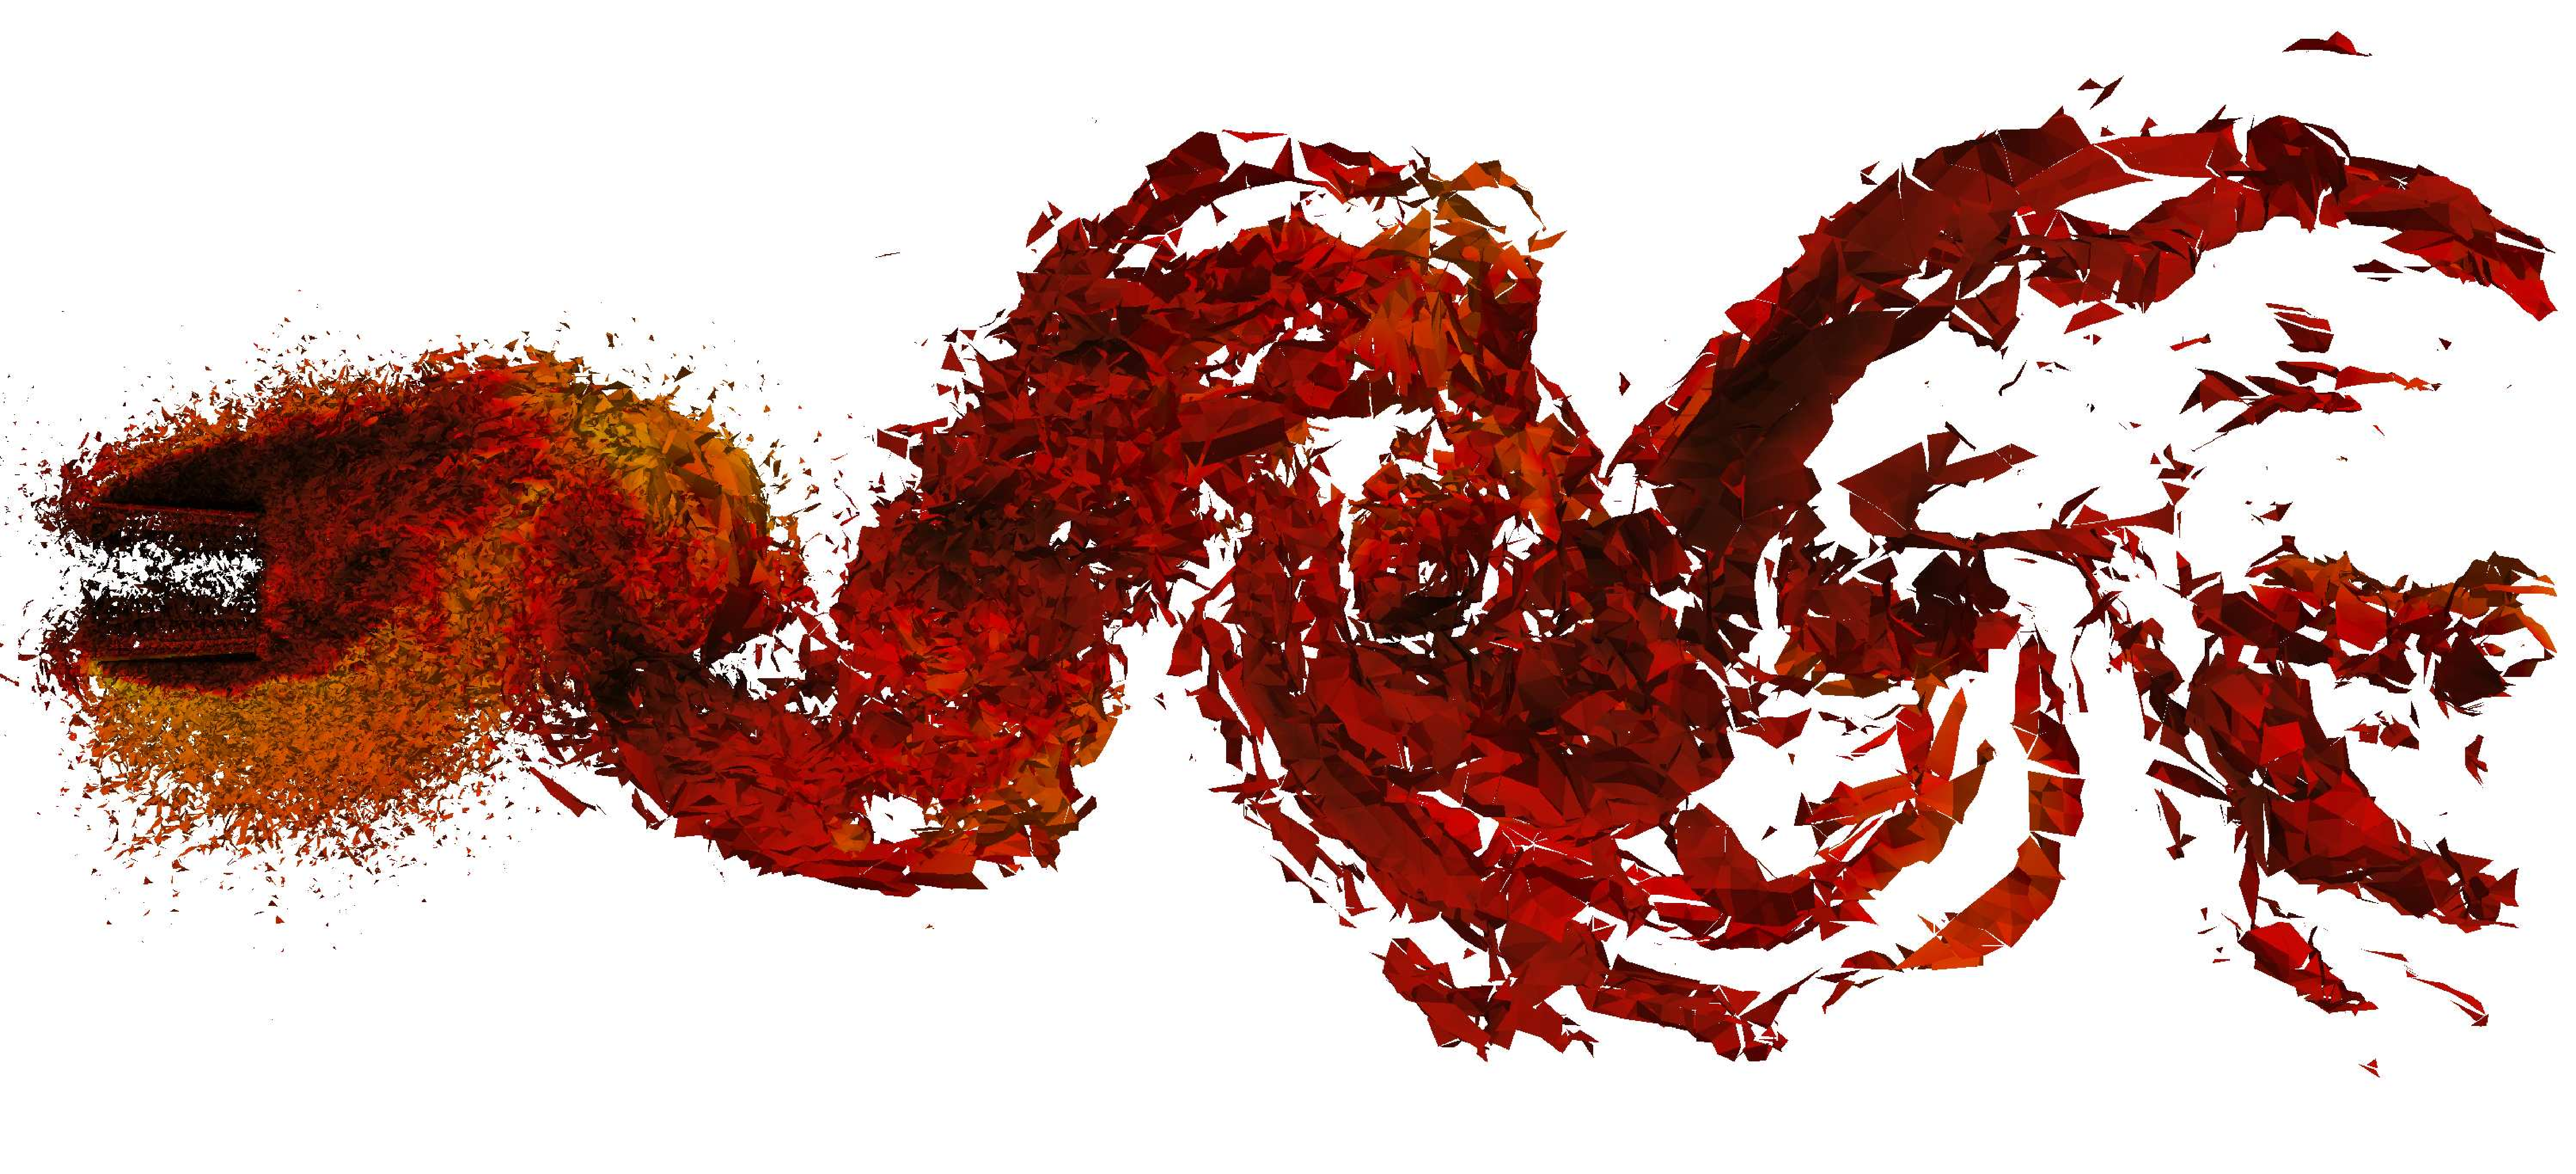
\includegraphics[width=0.9\textwidth]{sqcyl-tet-wsm-newwallfn-coarse3-qcrit-010-velomag.pdf}
\caption{Isosurface of the $q$-criterion colored by velocity magnitude showing the wake behind the square cylinder}
\label{sqcylqcrit}
\end{figure}

\begin{figure}[h]
\centering
\subfloat[Mean streamwise velocity $\langle u \rangle/u_B$]{
\includegraphics*[width=0.8\textwidth]{sqcyl-tet-wsm-newfilt-coarse-fixbc-meanu-vprofile-small.pdf}}\\
\subfloat[Mean vertical velocity $\langle v \rangle/u_B$]{
\includegraphics*[width=0.8\textwidth]{sqcyl-tet-wsm-newfilt-coarse-fixbc-meanv-vprofile-small.pdf}}\\
\subfloat[Mean Reynolds stress $\langle u'u' \rangle/u_B^2$]{
\includegraphics*[width=0.8\textwidth]{sqcyl-tet-wsm-newfilt-coarse-fixbc-meanuu-vprofile-small.pdf}}\\
\subfloat[Mean Reynolds stress $\langle u'v' \rangle/u_B^2$]{
\includegraphics*[width=0.8\textwidth]{sqcyl-tet-wsm-newfilt-coarse-fixbc-meanuv-vprofile-small.pdf}}
\caption{\small (a) Mean streamwise and vertical velocity and mean Reynolds stresses along vertical lines in the wake.
(---) current results, (- - - ) 4th order \gls{sd}+\gls{wsm} on hexahedral mesh by Lodato and Jameson~\cite{lodato2012b}, ($\circ$) \gls{ldv} experiments by Lyn et al.~\cite{lyn1994,lyn1995}.}
\label{sqcylplots}
\end{figure}



% !TEX root = ../thesis.tex
\graphicspath{{\aiaadir /figures_RANS_naca0012/}}% Set graphics path location

\subsection{NACA 0012 airfoil at 0$\degr$ angle of attack, Re = 6 million, Ma = 0.15}
In this section, the NACA 0012 airfoil is used to study the accuracy of the \gls{sa} turbulence model coupled with \gls{fr}. The NACA 0012 is commonly used as a validation case for all turbulence models and a large database of results are available at the NASA Turbulence Modeling Resource website. A $6,539$ element quad/triangle mixed mesh is used with a NACA 0012 airfoil of chord length $1.0$ and a farfield boundary $20$ chord lengths away. The results are compared with CFL3D and experimental results from Gregory \& O'Reilly~\cite{gregory1973low}.

\begin{figure}

    \subfloat[Zoomed view of the mixed element mesh near the NACA 0012 airfoil.]{\includegraphics[width = 0.5\textwidth]{NACA0012_Re6mil_mesh.eps}}
    \subfloat[X-momentum contours near the NACA 0012 airfoil]{\includegraphics[width = 0.5\textwidth]{NACA0012_Re6mil_alp0_momx.eps}}

  \caption{Turbulent flow past a NACA 0012 airfoil at \gls{re} = 6 million, \gls{ma} = 0.15, $\alpha = 0^{\circ}$ using \gls{fr} to recover 4th order accurate \gls{dg} method and the \gls{sa} turbulence model.}
  \label{RANS_naca0012}
\end{figure}

\begin{figure}
\centering
  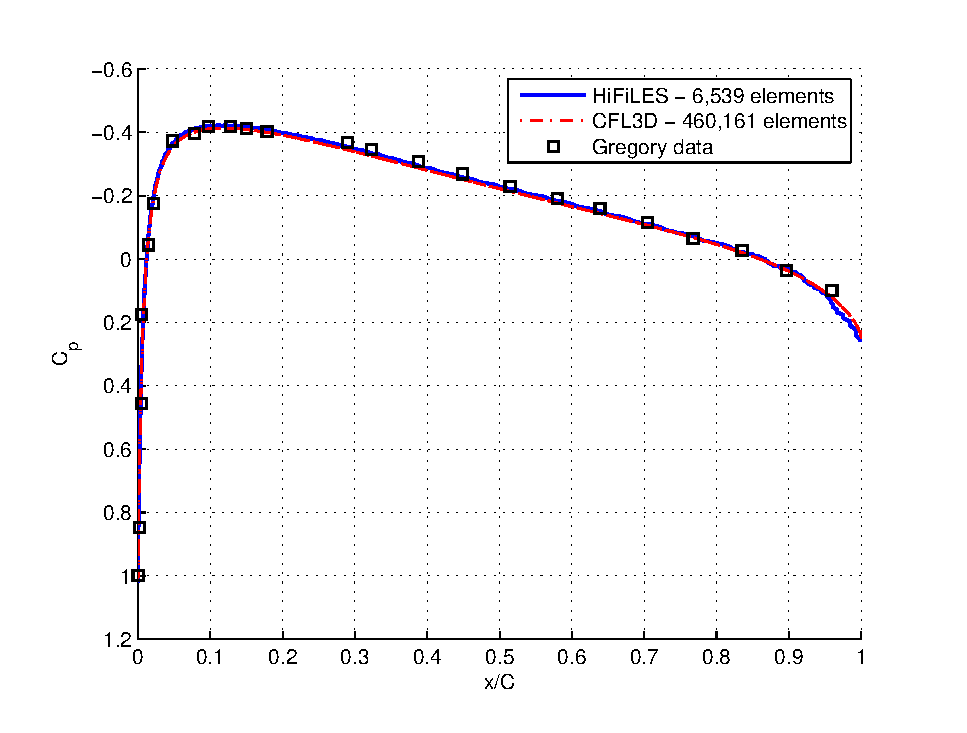
\includegraphics[width=0.48\textwidth]{cp.eps}
  \caption{Pressure coefficient on the NACA 0012 airfoil at \gls{re} = 6 million, \gls{ma} = 0.15, $\alpha = 0^{\circ}$ using \gls{fr} to recover 4th order accurate \gls{dg} method and the \gls{sa} turbulence model.}
  \label{RANS_naca0012_cp}
\end{figure}





% Note that the verification section above now has both V & V
%\section{Validation (Preliminary results)}
\label{sec:validation}
Here we follow some cases from the 2nd High-Order Workshop.

\subsection{Flat Plate}

\subsection{Circular Cylinder}
From David's thesis.



%\subsubsection{Vortex transport by uniform flow (2D)}
%\subsubsection{Transonic Ringleb Flow (2D)}
%\subsubsection{Flow over an Analytical Body of Revolution (3D)}

\subsection{RANS NACA 0012}

\subsection{SD7003 airfoil at 4$\degr$ angle of attack}
From David's thesis\cite{williams2013thesis}
\subsection{SD7003 wing section at 4$\degr$ angle of attack}
From David's thesis.
%\subsubsection{Laminar Flow around a Delta Wing}

\subsection{DNS of the Taylor-Green Vortex at Re = 1,600}

\begin{figure}
\centering
\includegraphics[height=60mm]{./figures/dissrate-hex-mesh-small.pdf} \\
\caption{LES of Tyalor-Green Vortex at Re=1,600\cite{bull2013a}}
\label{fig:setup}
\end{figure}


\subsection{DNS of Decaying Homogeneous Turbulence}
To be done by Manuel
\subsection{LES of Decaying Homogeneous Turbulence}
To be done by Manuel



% !TEX root = ./main.tex

\section{Conclusion}
\label{sec:conclusion_hf}

In this chapter, we have presented a comprehensive description, verification and validation of the \gls{hf} solver. In its first version, \gls{hf} offers to its users an optimal implementation of the \gls{fr} methodology in unstructured 3D grids using \gls{gpu}s or traditional \gls{mpi}. The implementation has been verified via \gls{mms}. The code has been tested in some difficult \gls{ns} and \gls{les} problems with very satisfactory results.

%pros:
The power of the \gls{fr} method is in its flexibility, efficiency and accuracy.
Different high-order schemes can be recovered by choosing a single parameter, allowing the numerical behavior to be fine-tuned.
%cons:
Though the use of explicit timestepping sets limits on the \gls{cfl} condition, the fact that \gls{hf} can be run on high performance multi-\gls{gpu} platforms more than compensates for this.


Despite considerable advances in the accuracy and versatility of \gls{sgs} models, current industrial \gls{cfd} codes are restricted in their ability to perform \gls{les} of turbulent flows by the use of highly dissipative second-order numerical schemes.
Therefore, in order to advance the state of the art in industrial \gls{cfd}, it is necessary to move to high-order accurate numerical methods.
The \gls{esfr} family of schemes are ideal for resolving turbulent flows due to low numerical dissipation and high-order accurate representation of solution gradients at the small scales.
Advanced subgrid-scale models have been implemented in \gls{hf} for all element types, enabling simulation of turbulent flows over complex geometry.
The development of the first high-order accurate solver for unstructured meshes incorporating \gls{les} modeling capabilities represents a significant step towards tackling challenging compressible turbulent flow problems of practical interest.
Future additions will include optimization of the \gls{esfr} schemes for turbulence resolution, moving mesh capabilities,  multigrid convergence acceleration, and advanced turbulence modeling.


\chapter{Flux Reconstruction Schemes with Corrected Fluxes Continuous in $m$ Derivatives}
\chaptermark{Provably-stable $C^m$ FR Schemes}

\section{Introduction}
The \gls{fr} approach to high-order methods provides a unifying framework to analyze and implement a large set of high-order schemes, including the nodal \gls{dg} and \gls{sd} methods. The unification occurs through the formulation of flux correction functions. The main appeal of \gls{fr} is its differential formulation, which is ideal for highly-parallel computational architectures. \gls{esfr} provides the added benefit of guaranteeing linear stability while having variable dispersion and dissipation properties parameterized by a single constant. Asthana~\cite{asthana2014high} found optimal values for such constant and found that the \gls{fr} scheme could be optimized further if the scheme's formulation were not constrained by this parameter.

With the intention of providing a framework whereby more parameters are introduced while linear stability is guaranteed, we formulate the $C^m$ Flux Reconstruction (CMFR) set of families of schemes. The main difference between \gls{esfr} and \gls{cmfr} is that the flux correction functions in \gls{cmfr} are forced to be continuous among elements in an arbitrary number of derivatives, while \gls{esfr} requires $C^0$ and $C^{p+1}$ continuity only --where $p$ is the degree of the polynomial used to discretize the solution.

In this article we present the proof of linear stability of the \gls{cmfr} set of families of schemes, the derivation of C1FR --a \gls{fr} scheme with $C^1$ correction functions--, and promising results for energy preservation of underresolved wavenumbers with C1FR.

\section{Background} 
High-order numerical methods for unstructured grids promise to offer better accuracy than low-order schemes for a comparable computational cost. Their relative lower dispersion and dissipation make them prime candidates for use in \gls{les}~\cite{lodato2014structural}. Below is a brief history on the developments in high-order numerical schemes that form the foundations for this chapter.

The work of Reed and Hill~\cite{reed73} in the 70's introduced the \gls{dg} method to solve \gls{pde}s in variational form. Cockburn and Shu formulated the \gls{dg} method for conservation laws and advanced its theoretical foundations \cite{cockburn1989tvbII,cockburn1989tvbIII,cockburn1990rungeIV,cockburn1989runge,cockburn2001runge}. As a way to reduce the computational cost of the original \gls{dg} scheme, researchers developed a nodal variant. Hesthaven and Warburton give a through exposition of this method in their book~\cite{hesthaven2007nodal}. Kopriva and Kolias~\cite{Kopriva96} developed a staggered grid method based on the differential form of the equations. This method was later named \gls{sd} and was thoroughly studied by Liu et al.~\cite{liu2006discontinuous} and Wang et al.~\cite{wang2007spectral}. Wang~\cite{wang2002spectral} has also introduced the popular spectral volume method.

Noting the similarities between nodal \gls{dg} and the \gls{sd} schemes, Huynh introduced the \gls{fr} approach to high-order methods \cite{huynh2007flux,huynh2009reconstruction}. With this approach, it is possible to analyze and implement multiple high-order schemes within a unifying framework, including the \gls{sd} method and a variant of nodal \gls{dg} for the linear advection equation. Furthermore, Huynh used the \gls{fr} approach to create a variety of new high-order schemes with different stability and accuracy properties. Vincent et al. \cite{vincent2011new}, building on Jameson's proof of stability of the \gls{sd} scheme \cite{jameson2010proof}, formulated a class of \gls{esfr} schemes. These schemes are provably stable at all orders of accuracy for the linear advection-diffusion equations \cite{castonguay2013energy}. Williams et al. and Castonguay et al. have proved this stability for all orders in tetrahedral \cite{williams2013tet} and triangular \cite{castonguay2012new,williams2013tri} meshes.

In the $p+1$th order \gls{fr} and \gls{esfr} schemes for the 1-dimensional linear advection equation, the solution is represented by a polynomial of degree $p$ and the flux is represented by a polynomial of degree $p+1$. In this article, we show that it is possible to represent the flux with a polynomial of degree $m$ -- where $m \ge p+1$--, evaluate such flux at the regular $p+1$ points, retain the provable linear stability, and obtain the expected $m+1$th order convergence (limited only by interpolation errors). An important part of the proof consists of ensuring that the flux polynomial representations have continuous arbitrary derivatives at the flux points connecting interfaces between elements, hence we call these schemes $C^m$ Flux Reconstruction (CMFR) schemes. This general framework recovers \gls{esfr} schemes and provides an arbitrary number of parameters that can be used to optimize the dispersion and dissipation properties of the schemes. The work by Asthana \cite{asthana2014high} shows how it is possible to optimize the dispersion and dissipation properties of \gls{esfr} schemes. His work inspired the formulation of a provably stable scheme with more optimizable parameters, and thus the creation of the \gls{cmfr} schemes presented here.

The article starts with the formulation of the \gls{cmfr} schemes. We then present the proof of stability for all orders of accuracy of the \gls{cmfr} schemes for the linear advection equation. The proof of stability requires the formulation of some ``correction functions", so the discussion continues with the general procedure for finding these. To illustrate the process of scheme creation, we show the development of the \gls{cmfr} scheme that has fluxes continuous in the $0$th and $1$st derivatives: the $C^{0,1}$\gls{fr} (or C1FR) scheme. We then perform numerical experiments that demonstrate the schemes' $p+1$th order convergence when we use an $p$th order polynomial to represent the flux. The discussion is followed by showing how the \gls{cmfr} schemes can preserve the energy of high-frequency waves better than the nodal \gls{dg} method at the price of exchanging flux derivative information across element interfaces and additional work in the simulation pre-processing stage. We conclude by showing potential avenues of future research.

\section{The $C^m$ Flux Reconstruction Approach}

\subsection{Preliminaries: the general advection equation}
Suppose we would like to solve the one-dimensional conservation law
\begin{equation}
\label{eq:advec}
\dd{u}{t} + \dd{f}{x} = 0 
\end{equation}
in the domain $\bOmega$. $x$ is the spatial coordinate, $t$ is time, $u = u(x,t)$ is the conserved scalar quantity (or solution), and $f=f(u)$ is the flux. 

To discretize the equation, let us partition $\bOmega$ into $N$ non-overlapping elements $\bOmega_n = \{x | x_n < x < x_{n+1}\}$ and approximate both the solution $u$  and flux $f$ within each $\bOmega_n$ with polynomials. In each element, solution points are the locations where the solution values are stored and advanced; flux points in each element serve the same purpose for the flux values. In the Flux Reconstruction family of schemes, the solution and flux points are collocated in order to not have to compute additional flux interpolations.

As is customary, let us map the approximated solution and flux from the physical domain $\bOmega_n$ in $x$-coordinates to the reference domain $\hat{\Omega}=\{\xi | -1 < \xi < 1\}$ in $\xi$-coordinates. We can then write the approximations in the following form
\begin{align}
 \urd &= \sum^{P+1}_{p=1} \urd_p l_p(\xi) \\ 
 \frd &= \sum^{P+1}_{p=1} \frd(\urd_p)l_p(\xi)
\end{align}
where $P$ is the polynomial order used to represent the solution, $l_p$ is the Lagrange polynomial that equals $1$ at the solution/flux point $p$ and $0$ at the others, and $\urd_p$ is the solution value at the point $p$. Note that both $u$ and $f$ are potentially discontinuous across elements. 
The circumflex $\wedge$ means that the polynomial or entity below it is written or defined in reference domain coordinates.

Understanding that $J_n = \ddxi{x}\big|_n$,
we can rewrite Eqn.~\eqref{eq:advec} the reference domain coordinates
\begin{equation}
 \dd{\urd}{t} + \frac{1}{J_n}\ddxi{\frd} = 0 
\end{equation}

Let us clearly show the values of the desired $m^{\text{th}}$ order derivatives at the left interfaces of the $n^{\text{th}}$ element in
both the physical and reference domains.
\begin{align}
f\big|^{I}_{L,n} &= \frd\big|^{I}_{L,n} \\
\dd{f}{x} \bigg|_{L,n}^I &= \frac{1}{J_n} \ddxi{\frd}  \bigg|_{L,n}^I\\
\dd{^m f}{x^m} \bigg|_{L,n}^I &= \frac{1}{J_n^m} \dd{^m \frd}{\xi^m}  \bigg|_{L,n}^I
\end{align}

Here the symbol $|^{I}_{n,L}$ denotes that the quantity to its left is being evaluated at the \emph{left} ($L$) \emph{interface} ($I$) of element $n$, and $J_n$ represents the Jacobian of element $n$. Note that the desired interface values $\dd{^m \frd}{\xi^m}  \big|_{L,n}^I$ and $\dd{^m \frd}{\xi^m}  \big|_{R,n}^I$ will be defined later on when proving linear stability of the scheme.

It is important to note that
\begin{equation}
\dd{^m f}{\xi^m}  \bigg|_{R,n}^I = \dd{^m f}{\xi^m}  \bigg|_{L,n+1}^I
\end{equation}

Eventually, we would like to add a polynomial to the flux in order to guarantee continuity of arbitrary derivatives across elements. To that end, let us define the following correction constants at the left interface of element $n$ --the correction constants at the right interface are defined in the same way by replacing $L$ with $R$--

\begin{equation} 
\begin{aligned}
 \text{for $c^0$ continuity:} \, \IL[0] &= 
f\big|^I_{L,n} - \fud\big|_{L,n}\\
&= \frd\big|^I_{L,n} - \frd\big|_{L,n}\\
 &\vdots\\
\text{for $c^m$ continuity:} \, \IL[m] &= %
\dd{^m f}{x^m} \bigg|^I_{L,n} - \dd{^m \fud}{x^m} \bigg|_{L,n}\\
&= \frac{1}{J_n^m}\l(\dd{^m \frd}{\xi^m} \bigg|^I_{L,n} - \dd{^m \frd}{\xi^m} \bigg|_{L,n}\r)
\end{aligned}
\label{eq:jump_def}
\end{equation}
These constants are the difference between the desired flux derivative and the derivative of the flux polynomial at the interface of interest.

We can now introduce the correction functions that will enforce flux derivative continuity across elements. To guarantee that we have full control over which derivatives will be continuous at both the left ($L$) and right ($R$) interfaces at each element, we set the following conditions on the correction functions $\gL(\xi)$ and $\gR(\xi)$ defined in
element $n$ as follows:
\begin{equation}
\label{eq:gconstraints}
\begin{split}
&\dd{^j \gL}{x^j}(-1) = \delta_{ij} \; ; \; \dd{^j \gL}{x^j}(1) =
0 \\
&\dd{^j \gR}{x^j}(-1) = 0 \; ; \; \dd{^j \gR}{x^j}(1) = \delta_{ij}
%\frac{1}{J^j_n}
\end{split}
\end{equation}
where $\delta_{ij}$ is the Kronecker delta. $i$ and $j$ belong to the set of derivatives in which we wish to have continuity. For example, if we desire flux continuity in the zeroth and third derivatives, $i,j \subset \{0,3\}$. Note that the correction function polynomials must be of order greater than or equal to $2s$, where $s$ is the number of derivative continuities desired, due to the existence of two constraints per correction function. In the previous example, $s=2$.

Putting all the definitions together, we can now define the corrected flux in element $n$ as
\begin{equation}
\label{eq:f_corrected}
 \frd^{c} = \frd + \sum^m_{i=0}\left\{ \IL \gL + \IR \gR
 \right\}
\end{equation}
where $m$ is the highest derivative in which continuity is desired. The superscript $c$ is used to make it explicit that the quantity over which it appears has been made continuous across element interfaces. In the example, $m=3$, $I_{1_{L,n}} = I_{1_{R,n}} = I_{2_{L,n}} = I_{2_{R,n}} = 0$.
The semi-discrete form of the update step in element $n$ is
\begin{equation}
\DD{\urd_p}{t} = -\frac{1}{J_n} \left[ \ddxi{\frd}(\xi_p) + \sum_{i=0}^m \left\{ \IL
\ddxi{\gL}(\xi_p) + \IR \ddxi{\gR}(\xi_p)\right\} \right]
\end{equation}
for $p = 1,\ldots,P+1$. Note that the correction functions are being sampled at the same points as the flux and solution, so the fact that we are using polynomials of high orders as correction functions does not add computational complexity to the update step.
In vector form,
\begin{equation}
\DD{\overrightarrow{\urd}}{t} = -\frac{1}{J_n} \left[ \overrightarrow{\ddxi{\frd}} + \sum_{i=0}^m
\left\{ \IL
\overrightarrow{\ddxi{{\gL}}} + \IR \overrightarrow{\ddxi{{\gR}}}\right\}
\right]
\end{equation}

Here we see more clearly that the scheme maintains the desired computational parallelizability of the Flux Reconstruction family of schemes, as the only element specific values are the scalars $J_n$, $\IR$ and $\IL$.

\subsection{CMFR schemes for the general advection-diffusion equation}
The extension of a \gls{fr} scheme for the advection equation to the advection-diffusion equation is straightforward. If we want to solve
\begin{equation}
\label{eq:adv_diff}
\dd{u}{t} + \dd{f}{x} + \frac{\partial ^2 h}{\partial x^2}= 0 
\end{equation}
where $f$ and $h$ are functions of $u$, we can introduce an auxiliary variable $q$ so the equation becomes
\begin{equation}
\begin{split}
\dd{u}{t} + \dd{q}{x} &= 0\\
q &= f + \dd{h}{x} 
\end{split}
\end{equation}
Note that in the linear case, $h = -\beta u$ and $f = a u$.


When solving any \gls{pde}, the \gls{cmfr} schemes correct all functions dependent on $u$ whose first derivatives need to be found. In this general advection-diffusion case, $q$ and $h$ need to be corrected following the form in Eqn. \eqref{eq:f_corrected}. The main difference between this and the advection equation \gls{cmfr} scheme is that in this case there are two corrections necessary and the interface values $\IL,\IR$ used to correct $q$ will be a function of $q = f + \dd{h}{x}$ and not just $f$. The correction functions found for Eqn. \eqref{eq:f_corrected} remain exactly the same.

\section{Linear stability of $C^m$ continuous flux reconstruction $(\frd = a\urd)$}

In this section we show that the \gls{cmfr} schemes are stable in the 1-D linear advection equation in the following Sobolev-type norm:
\begin{equation}\label{eq:norm}
\begin{split}
|| \uud ||^2_m &=\sum_{n=1}^{N}\int_{x_n}^{x_{n+1}} \l\{ \sum^m_{r=0}
\frac{c_r}{2} \l( \dd{^r \uud}{x^r} \r)^2 \r\} dx \\
&=\sum_{n=1}^{N}   \sum^m_{r=0}
c_r \l(  \frac{1}{J_n^{2r}}\r) \ioo \l\{ \frac{1}{2}\l(\ddxir{\urd}{r} \r)^2
\r\} J_n \cdot d\xi 
\end{split}
\end{equation}
where $c_r$ for $0 \le r \le m$ are arbitrary constants. %To ensure Eqn.~\eqref{eq:norm}
%is a norm, let $c_0=1$. 
It is possible to find ranges of values of each $c_r$ for which Eqn. \eqref{eq:norm} is a norm. As shown later in section \ref{sec:advDiff}, negative values of $c_r$ are possible given that $\uud$ is a polynomial. To establish stability, we need to show that
\begin{equation}
\label{eq:ddnorm}
\DD{}{t}||\uud||^2_m = \sum_{n=1}^{N}   \sum^m_{r=0}
c_r \l(  \frac{1}{J_n^{2r}}\r) \DD{}{t}\ioo \l\{ \frac{1}{2}\l(\ddxir{\urd}{r} \r)^2
\r\} J_n \cdot d\xi \le 0
\end{equation} 

To that end, consider the \gls{fr} scheme in element $n$ for linear advection:
\begin{equation}
\label{eq:scheme}
\DD{\urd}{t} = -\frac{1}{J_n} \left[ a\ddxi{\urd} + \sum_{i=0}^m
\left\{ \IL
\ddxi{\gL} + \IR \ddxi{\gR}\right\} \right]
\end{equation}

To express Eqn. \eqref{eq:norm} in known terms, differentiate Eqn.
\eqref{eq:scheme} $r$ times, where $0\le r\le m$, with respect to $\xi$;
multiply by $\ddxir{\urd}{r}$; and integrate from $-1$ to $1$ to obtain
\begin{equation}
\label{eq:normterm1}
 \DD{}{t}\ioo \l\{ \frac{1}{2}\l( \ddxir{\urd}{r} \r)^2  \r\} d\xi = -\frac{1}{J_n}
\l[\text{\ding{172}}+\text{\ding{173}}+\text{\ding{174}} \r]
\end{equation}
where
\begin{align}
\label{eq:exp1}
 \text{\ding{172}}&= a \ioo \frac{1}{2} \ddxi{}\l( \ddxir{\urd}{r}\r)^2 d\xi=\frac{a}{2}\l[ 
\l( \ddxir{\urd}{r}\r)^2\bigg|_{R,n} - \l( \ddxir{\urd}{r}\r)^2\bigg|_{L,n} \r]\\
\label{eq:normterm2}
\text{\ding{173}}&= \sum^m_{i=0} \IL \ioo \ddxir{\urd}{r}\cdot \ddxir{\gL}{r+1} d\xi\\
\text{\ding{174}}&= \sum^m_{i=0} \IR \ioo \ddxir{\urd}{r}\cdot \ddxir{\gR}{r+1} d\xi
\end{align}


It is possible to simplify Eqn. \eqref{eq:normterm2} further.
% \begin{equation}
%  \text{\ding{173}}= \sum^m_{i=0} \IL \ioo \ddxir{\urd}{r}\cdot \ddxir{\gL}{r+1}
% d\xi\\
% \end{equation}
Integrating by parts,
\begin{align}
 \text{\ding{173}}&=\sum^m_{i=0} \IL \l\{ \ioo \l( \ddxi{} \l[ \ddxir{\urd}{r}
\ddxir{\gL}{r} \r]
-\ddxir{\gL}{r} \ddxir{\urd}{r+1} \r) d\xi \r\}\\
\text{\ding{173}}&= \sum^m_{i=0} \IL \l[\ddxir{\urd}{r} \ddxir{\gL}{r}\r]^1_{-1}
- \sum^m_{i=0} \IL \ioo
\ddxir{\gL}{r} \ddxir{\urd}{r+1} d\xi
\end{align}
By using the boundary conditions on $\gL$ given in Eqn.
\eqref{eq:gconstraints},
\begin{equation}
\label{eq:exp2}
\text{\ding{173}}=-\IL[r] J_n^r \ddxir{\urd}{r}\bigg|_{L,n} - \sum^m_{i=0} \IL \ioo
\ddxir{\gL}{r} \ddxir{\urd}{r+1} d\xi 
\end{equation}
Proceeding similarly with term \ding{174}
\begin{equation}
\label{eq:exp3}
\text{\ding{174}}=\IR[r] J_n^r\ddxir{\urd}{r}\bigg|_{R,n} - \sum^m_{i=0} \IR \ioo
\ddxir{\gR}{r}
\ddxir{\urd}{r+1} d\xi
\end{equation}

Note the difference in signs between \ding{173} and \ding{174}.

By replacing the expression from Eqn.~\eqref{eq:normterm1} into Eqn.~\eqref{eq:ddnorm}, we
obtain
\begin{equation}
\begin{split}
\label{eq:newnorm}
 \DD{}{t}&||\uud||^2_m = \sum_{n=1}^{N}\bigg\{   
\sum^m_{r=0}c_r \l(  -\frac{1}{J_n^{2r}}\r)  \frac{a}{2}\l[\l(
\ddxir{\urd}{r}\r)^2\bigg|_{R,n} - \l(\ddxir{\urd}{r}\r)^2\bigg|_{L,n} \r]  \\
&+ \sum^m_{r=0} c_r \l( - \frac{1}{J_n^{2r}}\r)  \l[ -\IL[r] J_n^r\ddxir{\urd}{r}
\bigg|_{L,n} - \sum^m_{i=0} \IL \ioo \ddxir{\gL}{r} \ddxir{\urd}{r+1} d\xi\r]\\
&+ \sum^m_{r=0} c_r \l( - \frac{1}{J_n^{2r}}\r)  \l[ \IR[r] J_n^r\ddxir{\urd}{r}
\bigg|_{R,n} -\sum^m_{i=0} \IR \ioo \ddxir{\gR}{r} \ddxir{\urd}{r+1} d\xi\r]\bigg\}
\end{split}
\end{equation}

%Notes: $g$ can be of any order as long as boundary constraints are satisfied. In other words, as will be seen later, $g$ must be at least of order $2(s+1)$ where $s$ is the number of types of flux continuities desired. If $g$ is $\mathcal{O}(p+s) ,s>1 \rightarrow$  cannot include $p\th$ order terms (simply) unless $c^p$ continuous. 

To de-clutter the notation, let us define $$\ddxir{*}{r} = \dD{*}{r} $$ and re-arrange Eqn.~\eqref{eq:newnorm} to obtain
\begin{equation}
\label{eq:timenorm}
 \DD{}{t}||\urd||^2_m = \text{\textcircled{a}} + \text{\textcircled{b}} + \text{\textcircled{c}}
\end{equation}
where
\begin{equation}
\begin{split}
 \label{eq:simpNormA}
 \text{\textcircled{a}} = -\sum_{n=1}^{N}  \bigg\{& 
 \sum^m_{r=0} c_r  \frac{a}{2} 
 \l[ \urd^{{(r)}^2} \big|_{R,n} - \urd^{{(r)}^2} \big|_{L,n} \r] 
 \l( \frac{1}{J_n^{2r}} \r) \\
 +& \sum^m_{r=0} -c_r \IL[r] J_n^r\urd^{(r)} \big|_{L,n} \l(
\frac{1}{J_n^{2r}}\r)\\
 +& \sum^m_{r=0} c_r \IR[r] J_n^r\urd^{(r)} \big|_{R,n} \l( \frac{1}{J_n^{2r}}\r)
 \bigg\} 
\end{split}
\end{equation}
\begin{equation}\label{eq:b_def}
 \text{\textcircled{b}} = \sum_{n=1}^{N} \l\{ 
 \sum^m_{r=0} c_r \sum^m_{i=0} \IL \ioo \dD{\gL}{r} \hat{u}^{{ (r+1)}} d\xi \l(
\frac{1}{J_n^{2r}}\r) \r\}
\end{equation}
\begin{equation}\label{eq:c_def}
 \text{\textcircled{c}} = \sum_{n=1}^{N}  \l\{ 
 \sum^m_{r=0} c_r \sum^m_{i=0} \IR \ioo \dD{\gR}{r} \hat{u}^{{ (r+1)}} d\xi \l(
\frac{1}{J_n^{2r}}\r) \r\}
\end{equation}


We show stability of \gls{cmfr} in the two following steps:
\begin{enumerate}
 \item We show that for a selection of interface values $\IL $ and $\IR $, 
 \begin{equation}\label{eq:a_le_0}
\text{\textcircled{a}} \le 0
 \end{equation}
 \item We explain how to find functions $\gL $ and $\gR $, for $i = 0,\ldots,m $ satisfying
conditions \eqref{eq:gconstraints} such that
\begin{equation}\label{eq:bc_equal_0}
\begin{split}
\text{\textcircled{b}}&=0\\
\text{\textcircled{c}}&=0
\end{split}
\end{equation}  
 for arbitrary
$c_r, r=1,\ldots,m$.
\end{enumerate}

By showing that expressions \eqref{eq:a_le_0} and \eqref{eq:bc_equal_0} hold, we conclude, from Eqn. \eqref{eq:timenorm} that
\begin{equation}
\DD{}{t}||\urd||_m \le 0
\end{equation}

\subsection{Part 1.}

In this part of the proof, we aim to show that the term \textcircled{a} in
Eqn.~\eqref{eq:timenorm} is non-positive.
\\
Rearranging and factoring terms in \textcircled{a}, Eqn. \eqref{eq:simpNormA} becomes
\begin{equation}
\begin{split}
\text{\textcircled{a}} =& -\sum_{n=1}^{N}  \bigg\{
 \sum^m_{r=0} c_r \l( \frac{1}{J_n^{2r}}\r)
 \bigg( \frac{a}{2} 
 \l[ \hat{u}^{{(r)}^2} \big|_{R,n} - \hat{u}^{{ (r)}^2} \big|_{L,n} \r]\\
 &- \IL[r] J_n^r\cdot \dD{\urd}{r} \big|_{L,n}
 +   \IR[r] J_n^r\cdot \dD{\urd}{r} \big|_{R,n}  \bigg)
 \bigg\}
 \end{split}
 \label{eq:aterm}
\end{equation}

Recall the definition of the correction constants $\IL[r] $ and
$\IR[r]$ in element $n$ from Eqn. \eqref{eq:jump_def},
\begin{equation}
\begin{split}
 \IL[r]J_n^r &= \dD{f}{r} \big|^I_{L,n} - {f}^{ (r)} \big|_{L,n}\\
 \IR[r]J_n^r &= \dD{f}{r} \big|^I_{R,n} - {f}^{ (r)} \big|_{R,n}
\end{split}
\end{equation}

In the case of linear advection, $\hat{f}^\delta = a\urd$, so the correction constants become
\begin{equation}
\label{eq:lincor}
\begin{split}
 \IL[r]J_n^r &= \dD{\hat{f}}{r} \big|^I_{L,n} - a\urdrL\\
 \IR[r]J_n^r &= \dD{\hat{f}}{r} \big|^I_{R,n} - a\urdrR
\end{split}
\end{equation}

Let us introduce the following generalized Roe flux at the interfaces, so
\begin{equation}
\label{eq:ifluxdef}
\begin{split}
\dD{\hat{f}}{r} \big|^I_{L,n} = \frac{1}{2}& \l[a\urdrL[n] + 
a\urdrR[n-1] \r] \\
&- \frac{1-{\alpha_r}}{2} \l|A_{r_{L,n}}\r| \l[\urdrL - \urdrR[n-1] \r]\\
\dD{\hat{f}}{r} \big|^I_{R,n} = \frac{1}{2}& \l[a\urdrL[n+1] + 
a\urdrR[n] \r]\\
&- \frac{1-{\alpha_r}}{2} \l|A_{r_{R,n}}\r| \l[\urdrL[n+1] - \urdrR[n] \r]
\end{split}
\end{equation}

Where $A_{r_{L,n}}$ and $A_{r_{R,n}}$ are the Jacobian matrices corresponding to the
$r^{\text{th}}$ derivative of the flux at the left ($L$) and right ($R$) interfaces of element $n$.
Equivalently,
\begin{equation}
\begin{split}
 A_{r_{L,n}} &= \l[ \frac{d \big( \hat{f}^{(r)} \big)}{d \big( \hat{u}^{(r)} \big)}
\r]_{L,n}\\
 A_{r_{R,n}} &= \l[ \frac{d \big( \hat{f}^{(r)} \big)}{d \big( \hat{u}^{(r)} \big)}
\r]_{R,n}
\end{split}
\end{equation}

Numerically, $A_{r_{L,n}}$ and $A_{r_{R,n}}$ can be evaluated for the linear advection equation as
\begin{equation}
\begin{split}
 A_{r_{L,n}} &= \frac{a \urdrL[n] - a \urdrR[n-1]}{\urdrL[n] - \urdrR[n-1]} = a\\%\aL\\
 A_{r_{R,n}} &= \frac{a \urdrL[n+1] - a \urdrR[n]}{\urdrL[n+1] - \urdrR[n]} = a%\aR = \aL[n+1]
\end{split}
\end{equation}

% Note that in the case of linear advection, $\aR = \aL = a$ for all $n$ and $r$. We leave the
% subscripts to later show that \textcircled{a} is non-negative even when the flux in non-linear.

Note that $A_{r_{L,n}} = A_{r_{R,n-1}}$ even for non-linear fluxes by construction.

Plugging these values of $A_{r_{L,n}}$ and $A_{r_{R,n}}$ into Eqn. \eqref{eq:ifluxdef}, and
substituting the updated interface flux values $\dD{\hat{f}}{r} \big|^I_{L,n}$ and $\dD{\hat{f}}{r}
\big|^I_{R,n}$ into the definition of the interface correction values in Eqn. \eqref{eq:lincor},
we obtain

\begin{equation}
\begin{split}
 \IL[r] J_n^r = \frac{1}{2} &\l\{a\urdrL[n] + 
a\urdrR[n-1] \r\}\\
 &- \frac{1-{\alpha_r}}{2} \l|a\r| \l\{\urdrL - \urdrR[n-1] \r\} - a\urdrL\\
 \IR[r] J_n^r = \frac{1}{2} &\l\{a\urdrL[n+1] + 
a\urdrR[n] \r\} \\
&- \frac{1-{\alpha_r}}{2} \l|a\r| \l\{\urdrL[n+1] - \urdrR[n] \r\} - a\urdrR
\end{split}
\end{equation}

Simplifying,
\begin{equation}
\label{eq:lincorUpdated}
\begin{split}
 \IL[r] J_n^r= \frac{a}{2}& \l\{-\urdrL[n] + \urdrR[n-1] \r\} \\
 &- \frac{1-{\alpha_r}}{2} \l|a\r| \l\{\urdrL
- \urdrR[n-1] \r\} \\
 \IR[r] J_n^r= \frac{a}{2}& \l\{\mbox{\;\;\:} \urdrL[n+1] - \urdrR[n] \r\} \\
 &- \frac{1-{\alpha_r}}{2}
\l|a\r|\l\{\urdrL[n+1] - \urdrR[n] \r\} 
\end{split}
\end{equation}


Using the updated values of $\IL[r]$ and $\IR[r]$ from Eqn. \eqref{eq:lincorUpdated},
Eqn. \eqref{eq:aterm} becomes
\begin{equation}
\begin{split}
 \text{\textcircled{a}} = -\sum_{n=1}^{N}  \bigg\{
 \sum^m_{r=0} & c_r \l( \frac{1}{J_n^{2r}}\r)
 \bigg( \frac{a}{2} 
 \l[ \hat{u}^{{ (r)}^2} \big|_{R,n} - \hat{u}^{{ (r)}^2} \big|_{L,n} \r] \\
 %
 &- \bigg[ \frac{a}{2} \l\{-\urdrL[n] + \urdrR[n-1] \r\} \\
 &\mbox{\;\;\;} - \frac{1-{\alpha_r}}{2} \l|a\r| \l\{\urdrL
- \urdrR[n-1] \r\} \bigg]  \cdot \urdrL\\
 &+  \bigg[ \frac{a}{2} \l\{\mbox{\;\;\:} \urdrL[n+1] - \urdrR[n] \r\} \\
 &\mbox{\;\;\;} - \frac{1-{\alpha_r}}{2} 
\l|a\r|
\l\{\urdrL[n+1] - \urdrR[n] \r\} \bigg]
 \cdot \urdrR 
\bigg)
 \bigg\} 
\end{split}
\end{equation}


Distributing the $\l(\frac{1}{J_n^{2r}}\r)$ term to convert the derivatives with respect to $\xi$
into derivatives with respect to $x$, and factoring out the $ \frac{a}{2}$ term,

\begin{equation}
\label{eq:termaphys}
\begin{split}
 \text{\textcircled{a}} = -\sum_{n=1}^{N}  \bigg\{
 \sum^m_{r=0} & c_r \frac{a}{2}
 \bigg(  
 \l[ {u}^{{ (r)}^2} \big|_{R,n} - {u}^{{ (r)}^2} \big|_{L,n} \r] \\
 %
 &- \bigg[ \l\{-\uudrL[n] + \uudrR[n-1] \r\} \\
 &\mbox{\;\;\;} - \frac{1-{\alpha_r}}{a} \l|a\r| \l\{\uudrL -
\uudrR[n-1] \r\} \bigg]
%
 \cdot \uudrL\\
 &+  \bigg[ \l\{\mbox{\;\;\:} \uudrL[n+1] - \uudrR[n] \r\} \\
 &\mbox{\;\;\;}- \frac{1-{\alpha_r}}{a} \l|a\r|
\l\{\uudrL[n+1] - \uudrR[n] \r\} \bigg]
 \cdot \uudrR 
\bigg)
 \bigg\} 
\end{split}
\end{equation}
%where the superscript $(r)$ now represents the $r^\text{th}$ derivative with respect to $x$.

Note that all terms in Eqn.~\eqref{eq:termaphys} are defined at element interfaces. More explicitly,
\begin{equation}
\label{eq:uudIdentities}
\begin{split}
\uudrL &= \uud_n(x_n) \\
\uudrR &= \uud_n(x_{n+1})
\end{split}
\end{equation}
where $\uud_n$ is the polynomial representing the solution in element $n$ and $x_n$ is the location
of the $n^\text{th}$ interface in physical coordinates.
Using the identities in Eqn.~\eqref{eq:uudIdentities}, Eqn.~\eqref{eq:termaphys} becomes
\begin{equation}
\label{eq:telSum0}
\begin{split}
 \text{\textcircled{a}} &= -\sum_{n=1}^{N}  \bigg\{
 \sum^m_{r=0} c_r \frac{a}{2}
 \bigg(  
 \l[ \l\{\uudrx{n}{n+1}\r\}^2  - \l\{\uudrx{n}{n}\r\}^2 \r] \\
 %
 &- \bigg[ \l\{-\uudrx{n}{n} + \uudrx{n-1}{n} \r\} \\
 &\mbox{\;\;\;}- \frac{1-{\alpha_r}}{a} \l|a\r|
\l\{\uudrx{n}{n} 
-
\uudrx{n-1}{n} \r\} \bigg]
%
 \cdot \uudrx{n}{n}\\
 &+  \bigg[ \l\{ \uudrx{n+1}{n+1} - \uudrx{n}{n+1} \r\} \\
 &\mbox{\;\;\;}- \frac{1-{\alpha_r}}{a} \l|a\r|
\l\{\uudrx{n+1}{n+1} - \uudrx{n}{n+1} \r\} \bigg]
 \cdot \uudrx{n}{n+1} 
\bigg)
 \bigg\} 
\end{split}
\end{equation}

Let us do the following substitutions to simplify algebraic manipulations
\begin{equation}
\label{eq:Bn}
\begin{split}
B_n = \sum^m_{r=0} c_r \frac{a}{2} \bigg( &\l[\uudrx{n-1}{n}\r]^2  \\
+ & \bigg[ \l\{\uudrx{n}{n} - \uudrx{n-1}{n} \r\} \\
&\mbox{\;\;\;}- \frac{1-{\alpha_r}}{a} \l|a\r| \l\{\uudrx{n}{n} 
- \uudrx{n-1}{n} \r\} \bigg] \cdot \uudrx{n-1}{n} \bigg)
\end{split}
\end{equation}

\begin{equation}
\label{eq:Dn}
\begin{split}
 D_n = \sum^m_{r=0} c_r \frac{a}{2} \bigg(- &\l[\uudrx{n}{n}\r]^2 \\
 - & \bigg[ \l\{-\uudrx{n}{n} + \uudrx{n-1}{n} \r\} \\
 &\mbox{\;\;\;}- \frac{1-{\alpha_r}}{a} \l|a\r|
\l\{\uudrx{n}{n} 
- \uudrx{n-1}{n} \r\} \bigg] \cdot \uudrx{n}{n} \bigg)
\end{split}
\end{equation}



We can then rewrite Eqn.~\eqref{eq:telSum0} as
\begin{equation}\label{eq:simple_summation}
  \text{\textcircled{a}} = -\sum_{n=1}^{N} \l\{ B_{n+1} + D_{n} \r\} 
\end{equation}

Let us manipulate \eqref{eq:simple_summation} to combine the two summations into one whose terms have the same unshifted index
\begin{equation}
\begin{split}
  \text{\textcircled{a}} &=  - \sum_{n=1}^{N} D_{n} -\sum_{n=1}^{N}  B_{n+1} \\
  \text{\textcircled{a}} &= - \sum_{n=1}^{N} D_{n} -\sum_{n=2}^{N+1}  B_{n}  \\
  \text{\textcircled{a}} &= - D_{1} - \sum_{n=2}^{N} D_{n}  - \sum_{n=2}^{N}  B_{n}  - B_{N+1} \\
  \text{\textcircled{a}} &= - D_{1} - \sum_{n=2}^{N} \l\{ D_{n}  +  B_{n} \r\}  - B_{N+1}
\end{split}
\end{equation}

Note that various terms in $B_n$ and $D_n$ cancel when summed (compare \eqref{eq:Bn} and \eqref{eq:Dn}). After doing such cancellations,
Eqn.~\eqref{eq:telSum0} becomes
\begin{equation}
 \text{\textcircled{a}} = -D_1 - \sum_{n=2}^{N} \sum^m_{r=0} c_r
\cdot \frac{1-\alpha_r}{2} |a| \l(\uudrx{n-1}{n} - \uudrx{n}{n} \r)^2 - B_{N+1} 
\end{equation}

The value of the solution and its derivatives at $x_1$ and $x_{N+1}$ are set by the desired boundary conditions. Both $D_1$ and $B_{N+1}$ depend exclusively on such pre-determined conditions:
% \begin{equation}
%  \uudrx{n}{n} = \uudrx{n-1}{n}
% \end{equation}
% As a result,
\begin{align}
 D_1 &= -\sum^m_{r=0} c_r\frac{a}{2} \l[ \uudrx{1}{1}\r]^2 \\
 B_{N+1} &= \sum^m_{r=0} c_r\frac{a}{2} \l[ \uudrx{N}{N+1}\r]^2
\end{align}

To not introduce/extract energy into/from the solution, let us set periodic boundary conditions in all derivatives,
\begin{equation}
 \uudrx{1}{1} = \uudrx{N}{N+1}
\end{equation}

Consequently, $D_1 + B_{N+1} = 0$, and Eqn.~\eqref{eq:telSum0} becomes simply
\begin{equation}
 \text{\textcircled{a}} = - \sum_{n=2}^{N} \sum^m_{r=0} c_r
\cdot \frac{1-\alpha_r}{2} |a| \l(\uudrx{n-1}{n} - \uudrx{n}{n} \r)^2
\end{equation}

Knowing that the following holds,
\begin{equation}
 \begin{split}
  c_r &\ge 0\\
  0 \le \alpha_r &\le 1\\
  \l(\uudrx{n-1}{n} - \uudrx{n}{n} \r)^2 &\ge 0  \mbox{ for } 2\le n \le N
 \end{split}
\end{equation}

we conclude that
\begin{equation}
 \text{\textcircled{a}} \le 0
\end{equation}


We have shown that the term \textcircled{a} in Eqn.~\eqref{eq:timenorm} is non-positive,
concluding this part of the proof.


\subsection{Part 2.}
We wish to find functions $\gL $ and $\gR $, for $i = 0,\ldots,m $,
which satisfy the boundary conditions in Eqn.~\eqref{eq:gconstraints} and the stability conditions of Eqn. \eqref{eq:bc_equal_0} (\textcircled{b}$=0$
and \textcircled{c}$=0$) for arbitrary
$c_r, r=1,\ldots,m$.

We start by finding $\gL$. Let us manipulate \textcircled{b} in Eqn. \eqref{eq:b_def} to find restrictions on $\gL$,

% done: 09/24/2014
\begin{equation}
\begin{split}\label{eq:b_cond}
 \text{\textcircled{b}} = \sum_{n=1}^{N} \l\{ 
 \sum^m_{r=0} \l[ c_r \l(
 \frac{1}{J_n^{2r}}\r) \sum^m_{i=0} \l( \IL \ioo \dD{\gL}{r} \hat{u}^{{ (r+1)}} d\xi \r) \r] \r\} &=0 \\
 = \sum_{n=1}^{N} \l\{ 
  \sum^m_{i=0} \l[ \IL \sum^m_{r=0} \l( c_r 
  \frac{1}{J_n^{2r}}  \ioo \dD{\gL}{r} \hat{u}^{{ (r+1)}} d\xi \r) \r] \r\} &=0
 \end{split}
\end{equation}

To satisfy Eqn. \eqref{eq:b_cond}, either
\begin{equation}
\label{eq:optionA}
\sum^m_{i=0}\l( \IL \ioo \dD{\gL}{r} \hat{u}^{{ (r+1)}}
d\xi \r) =0 
\end{equation}
or
\begin{equation}\label{eq:optionB}
\sum^m_{r=0} \l( c_r 
  \frac{1}{J_n^{2r}}  \ioo \dD{\gL}{r} \hat{u}^{{ (r+1)}} d\xi \r) =0
\end{equation}


We then have two options for finding $\gL$. Observing that the only term in the summand in \eqref{eq:optionB} that changes as the solution evolves is $\urd$ itself, we realize that a generic $\gL$ with special polynomial orthogonality properties would satisfy Eqn. \eqref{eq:b_cond}. As a result, we could pre-compute a non-changing $\gL$ to run a linearly stable scheme. On the other hand, the option given by \eqref{eq:optionA} obliges us to find
$\gL$ at every time-step because the scalar $\IL[i]$ changes with the solution. Therefore, we choose to find
$\gL$ using \eqref{eq:optionB}. %:
%\begin{equation}
%\label{eq:glcond}
% \sum^m_{r=0} c_r   \ioo \dD{\gL}{r} \hat{u}^{{\delta (r+1)}} d\xi \l(
%\frac{1}{J_n^{2r}}\r) =0 \text{ for each element $n$}
%\end{equation}


Rewriting $\urd$ as a sum of scaled Lagrange polynomials, condition \eqref{eq:optionB} becomes
\begin{equation}
 \label{eq:glcond1}  \sum^{P+1}_{p=1} \urd_p \sum^m_{r=0} \frac{c_r}{J^{2r}_n} \l(\ioo \dD{\gL}{r}
\dD{l_p}{r+1} d\xi \r) = 0
\end{equation}

This implies that
\begin{equation}\label{eq:glcond}
\sum^m_{r=0}\frac{c_r}{J^{2r}_n} \ioo \dD{\gL}{r} \dD{l_p}{r+1} d\xi = 0 
\end{equation}
for $p=1,\ldots, P+1$, (recall $P$ is the order of the polynomial used to represent $\urd$).
Let us expand the Lagrange polynomials $l_p$ and the correction functions $\gL$ into monomials,
\begin{equation}
\begin{split}
 l_p&=\sum^P_{j=0} \zeta_{pj} \xi^j\\
 \gL &= \sum^S_{k=0} \theta_{ik} \xi^k 
 \end{split}
\end{equation}
Note that $\zeta_{pj}$ are known, unchanging scalars while $\theta_{ik}$ are the unknowns we are trying to find. $S$ is the desired polynomial order of the correction function.

Eqn.~\eqref{eq:glcond} becomes
 \begin{equation*}
\sum^m_{r=0} \frac{c_r}{J^{2r}_n} \ioo 
\l( \sum^S_{k=r} \theta_{ik} \frac{k!}{(k-r)!} 
\xi^{k-r}  \r)
\l(
\sum^P_{j=r+1}\zeta_{pj}\frac{j!}{(j-r-1)!}  \xi^{j-r-1} \r)
d\xi =0
\end{equation*}

After some algebraic manipulation, we arrive at the conditions that each $\gL$ must satisfy so the \gls{cmfr} scheme maintains linear stability:
\begin{equation}
 \label{eq:gcond}
\sum^m_{r=0} \frac{c_r}{J^{2r}_n}  
\l[ \sum^S_{k=r} \theta_{ik} \frac{k!}{(k-r)!} 
\l(
\sum^P_{j=r+1}\zeta_{pj}\frac{j!}{(j-r-1)!}  \ioo \xi^{j+k-2r-1} d\xi\r)\r]
 =0
\end{equation}

Recall that $i$ in $\theta_{ik}$ indexes the correction function corresponding to each specific derivative in which continuity is desired. $p$ indexes each solution point in the reference domain.

With Eqn.~\eqref{eq:gcond} and the constraints given in Eqn.~\eqref{eq:gconstraints} we can
construct a system of equations to solve for $\gL$ in each element. More specifically, if we
would like to ensure $s$ different flux continuities between elements, the boundary constraints in
Eqn.~\eqref{eq:gconstraints} produce $2s$ equations, and the conditions in
Eqn.~\eqref{eq:gcond} produce $P$ equations (not necessarily all independent), where $P$ is the order of the solution
representation $\urd$. %Note, however, that if the flux continuity is desired in the $P+1^\text{th}$, or higher, derivative, the flux can be of order $2s+P-1+(-2)$ or higher, as the boundary conditions related to the $P+1^\text{th}$ derivative are satisfied automatically due to the fact that $\hat{u}^{\delta(P+1)}=0$ in every element.

We can recover the \gls{esfr} scheme by
ensuring continuity in the $0^\text{th}$ and $P+1^\text{th}$ derivatives. These two desired
flux continuities ($s=2$) force the flux to be of order, at least, $P+1$. This is the order of the correction functions suggested by Vincent~\cite{vincent2011new}. The \gls{esfr} scheme is one of the cases in which Eqn. \eqref{eq:glcond} produces $P-1$ independent equations instead of $P$. This can be seen by the fact that the $P+1^\text{th}$ and  $P+2^\text{th}$ derivatives of a Lagrange polynomial $l_p$ of order $P$ is zero.

Once we find $\gL$, we find $\gR$ automatically by setting 
\begin{equation}\label{eq:gr_gl_cond}
 \gR = (-1)^i\gL(-\xi)
\end{equation}
%in Eqn. \eqref{eq:c_def}.

\section{$C^{1}$ linearly stable flux reconstruction family of schemes}
In this section, we illustrate the process of creating a scheme that ensures $C^{1}$
flux continuity to solve the advection and advection-diffusion equation. This scheme is called C01FR, or \gls{c1fr}. We use this notation because it is possible to create a scheme whose reconstructed flux is continuous in the, say, zeroth and third derivatives without enforcing continuity in the first and second derivatives, and such scheme would have a $C^{0,3}$ flux and be called C03FR. When a scheme ensures continuity in the $0,\dots,M$ derivatives of the flux, we call it \gls{cmfr} to simplify the name, which could as well be C012...MFR.

\subsection{C1FR for the linear advection equation}
To create the scheme with $C^{1}$ flux, we only need to find correction functions $\gL$ that satisfy \eqref{eq:gcond} and boundary conditions \eqref{eq:gconstraints}.
Let $c_0$ and $c_1$ be non-zero in Eqn. \eqref{eq:gcond}. Expanding the summation over $r$, we have the following $P+1$ equations for each $i$

\begin{equation}
\begin{split}
c_0 &\l[ \sum^S_{k=0} \theta_{ik}\l( \sum^P_{j=1}\zeta_{pj}\cdot j\cdot \ioo  \xi^{j+k-1}d\xi \r) \r] \\
&+ 
\frac{c_1}{J^2_n} \l[ \sum^S_{k=1} k \theta_{ik} \l( \sum^P_{j=2}\zeta_{pj}\cdot j\cdot (j-1)\cdot \ioo  \xi^{j+k-3}d\xi \r) \r]
 = 0
 \end{split}
\end{equation}
for $p = 1,...,P+1$.

Rearranging terms we obtain
\begin{equation}
\begin{split}
\sum^P_{j=1} \zeta_{pj} &\bigg[ \sum^S_{k=0} \theta_{ik}\bigg( c_0\cdot  j \ioo  \xi^{j+k-1}d\xi  \\
&+ \frac{c_1}{J^2_n} k j\cdot (j-1)  \ioo  \xi^{j+k-3}d\xi \bigg) \bigg]
 = 0
 \end{split}
\end{equation}

and, therefore we have the following $P$ equations, where $j = 1,\dots,P$,
\begin{equation}
\label{eqn:system}
\sum^S_{k=0} \theta_{ik}\l( c_0\cdot  j \ioo  \xi^{j+k-1}d\xi  + \frac{c_1}{J^2_n} k j\cdot (j-1)  \ioo  \xi^{j+k-3}d\xi \r) = 0
\end{equation}

We can evaluate the integral terms understanding that for positive integer $q$
\begin{equation}
\ioo \xi^q d\xi = 
\l\{
\begin{array}{ll}
\frac{2}{q+1} & \mbox{, $q$ even}\\
0 & \mbox{, $q$ odd} 
\end{array}
\r.
\end{equation}

\begin{comment}
\begin{align}
 \ioo& \l\{ \gL\xi + \frac{c_1}{J_n^2} \ddxi{\gL}(j-1)\r\}\xi^{j-2} d \xi =0 \mbox{ for }
j=1,\ldots,m\\
 \implies &\sum^s_{k=0}\theta_{ik} \ioo \l\{ \xi^{k+1} + \frac{c_1}{J_n^2} k
\xi^{k-1}(j-1)\r\}\xi^{j-2}d\xi =0
\end{align}

We want to evaluate
\begin{equation}
 \ioo \l\{ \underbrace{\xi^{k+j-1}}_{\text{\ding{172}}} + \underbrace{\frac{c_1}{J_n^2} k (j-1)
\xi^{k+j-3}}_{\text{\ding{173}}} \r\} d\xi \mbox{ , } 0\le k\le s
\end{equation}

\ding{172}:

\begin{equation}
\ioo \xi^{k+j-1} d\xi = \frac{1}{k+j} \xi^{k+j} \bigg|^1_{-1} = \frac{1}{k+j} \l[ 1-(-1)^{k+j} \r]
\end{equation}

\ding{173}:
\begin{equation}
 \frac{1}{J_n^2}\ioo c_1 k (j-1) \xi^{k+j-3} d\xi = \frac{c_1}{J_n^2} k (j-1) \frac{1}{k+j-2} \l[
1-(-1)^{k+j-2} \r] \mbox{ for
} k+j\ne2
\end{equation}
If $k+j=2$, $j=2$ and $k=0$, so
\begin{equation}
 \ioo c_1 k (j-1) \xi^{k+j-3} d\xi = 0
\end{equation}

To find the coefficients of the monomials that describe $\gL$ and $\gR$, we want to write the
constraints in matrix form:
\begin{equation}
\label{eq:gcoeff}
 0=\sum^s_{k=0} \theta_{ik} \l\{  \frac{1}{k+j} \l[1-(-1)^{k+j}\r] + \frac{c_1}{J_n^2} k
\frac{j-1}{k+j-2} \l[
1-(-1)^{k+j-2} \r] \r\} \mbox{  for  } j=1,\ldots,p
\end{equation}

Note that for $j$ odd, Eqn.~\ref{eq:gcoeff} becomes
\begin{equation}
 0 = \sum^s_{\substack{k=0\\k \text{ even}}} \theta_{ik} \l\{ \frac{2}{k+j} +2 \frac{c_1}{J_n^2} k
\frac{j-1}{k+j-2}\r\}
\end{equation}

and for $j$ even, Eqn.~\ref{eq:gcoeff} becomes
\begin{equation}
 0 = \sum^s_{\substack{k=0\\k \text{ odd}}} \theta_k \l\{ \frac{2}{k+j} +2 \frac{c_1}{J_n^2} k
\frac{j-1}{k+j-2}\r\}
\end{equation}
\end{comment}
Recalling the constraints on $\gL$,
\begin{equation}
 g^{(j)}_{L_i}(-1) = \delta_{ij} J_n^j \; ; \;   g^{(j)}_{L_i}(+1) = 0
\end{equation}

we can obtain additional equations for each $\theta_{ik}$. Specifically, for $\gL[0]$,
\begin{equation}
\begin{split}
\sum^S_{k=0} \theta_{0k}(-1)^k = 1\hspace{0.7cm} \text{ \hspace{1cm} }
&\sum^S_{k=0}
\theta_{0k}(1)^k = 0\\
\sum^S_{k=1} k\theta_{0k}(-1)^{k-1} = 0 \text{ \hspace{1cm} } &\sum^S_{k=1}
k\theta_{0k}(1)^{k-1} = 0
\end{split}
\end{equation}
and for $\gL[1]$,

\begin{equation}
\begin{split}
\sum^S_{k=0} \theta_{1k}(-1)^k = 0\hspace{0.7cm} \text{ \hspace{1cm} }
&\sum^S_{k=0}
\theta_{1k}(1)^k = 0\\
\sum^S_{k=1} k\theta_{1k}(-1)^{k-1} = J_n \text{ \hspace{1cm}} & \sum^S_{k=1}
k\theta_{1k}(1)^{k-1} = 0
\end{split}
\end{equation}

From Eqn. \eqref{eq:gr_gl_cond}, we can find $\gR$ by setting
\begin{equation}
\gR = (-1)^i\sum_{k=0}^S \theta_{ik}(-\xi)^k = \sum_{k=0}^S \theta_{ik}(-1)^{i+k}\xi^k
\end{equation}

As a result, for each $\gL$ we have $P+4$ equations. By setting $S$, the order of the correction function, to be $P+3$, we have $P+4$ unknowns and can solve a $(P+4)\times(P+4)$ system of equations to have a one-parameter, linearly stable, $C^{1}$ flux, \gls{fr} scheme.

Letting the polynomial order $P$ be $3$, we obtain the correction functions seen in Fig. \ref{fig:c1_corfunc} for varying values of $c_1$. We let $c_0 = 1$ without loss of generality (as seen by the fact that in Eqn. \eqref{eqn:system} only the ratio $c_1/c_0$ modifies the correction functions). We note that the correction functions that ensure the flux is continuous in its first derivative, namely $\gL[1]$ and $\gR[1]$ are unaffected by changes in $c_1$. On the other hand, $\gL[0]$ and $\gR[0]$ change dramatically with changes in $c_1$. In section \ref{sec:num_cases} we will see how these variations affect dispersion and dissipation properties qualitatively.

In Fig. \ref{fig:c2_corfunc} we see the correction functions corresponding to the C012FR, or C2FR, scheme with $P=3$. It is interesting to note that changes in $c_1$ affect $\gL[0]$ and $\gR[0]$ only, changes in $c_2$ affect $\gL[1]$ and $\gR[1]$ only, and $\gL[2]$ and $\gR[2]$ are not affected by $c_1$ or $c_2$.

\begin{figure}[h]
\hspace{-1.25 cm}
\centering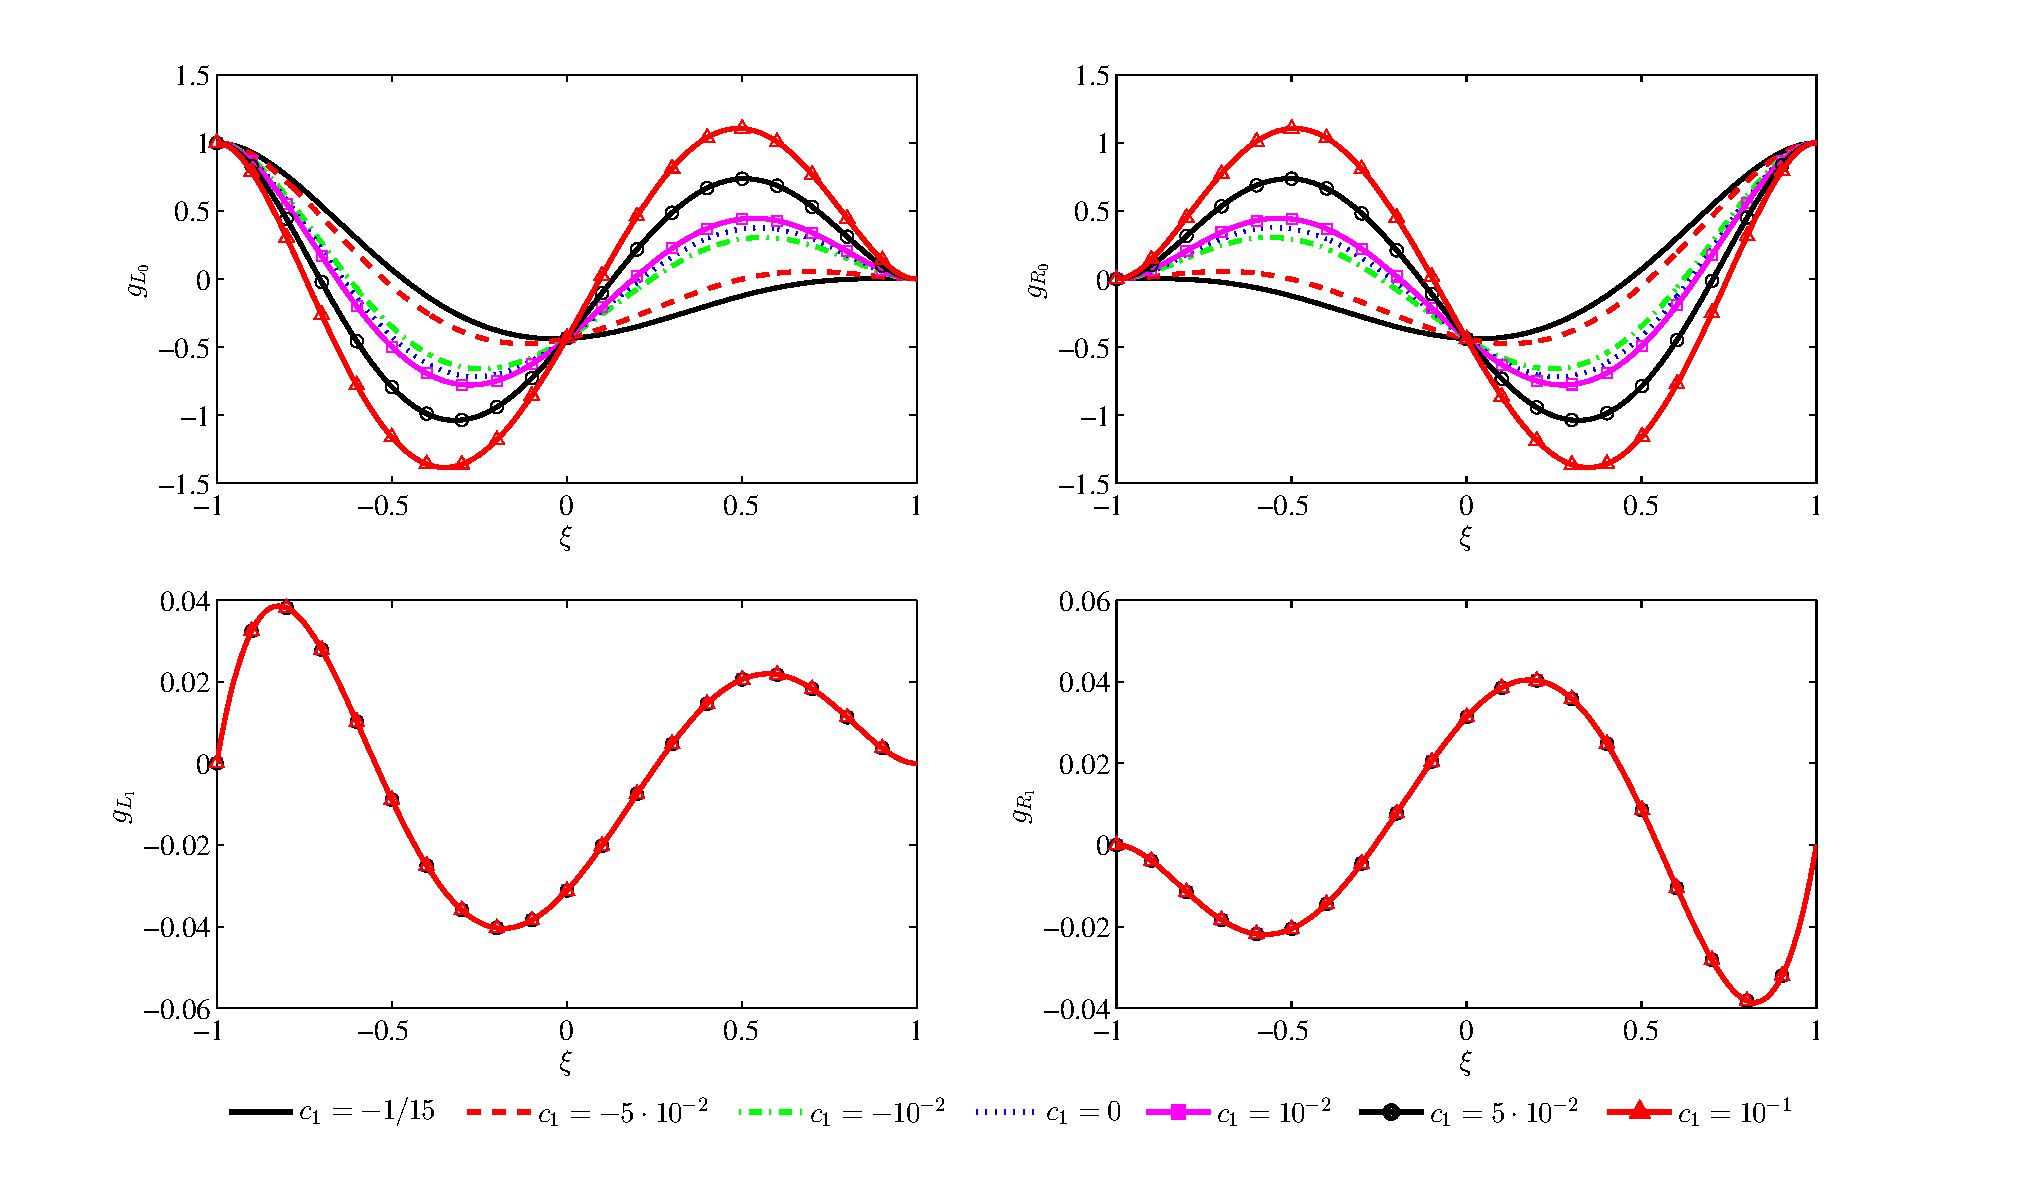
\includegraphics[width=\graphWidth\textwidth,trim=\Ltrim cm 0cm \Rtrim cm 0cm]{\cmfrdir/Figures/Correction_funcs/C1FR}
\caption{Left and right correction functions for the C1FR scheme with $P=3$, in which the zeroth and first derivatives of the corrected flux are continuous}
\label{fig:c1_corfunc}
\end{figure}

\begin{figure}[h]
\centering 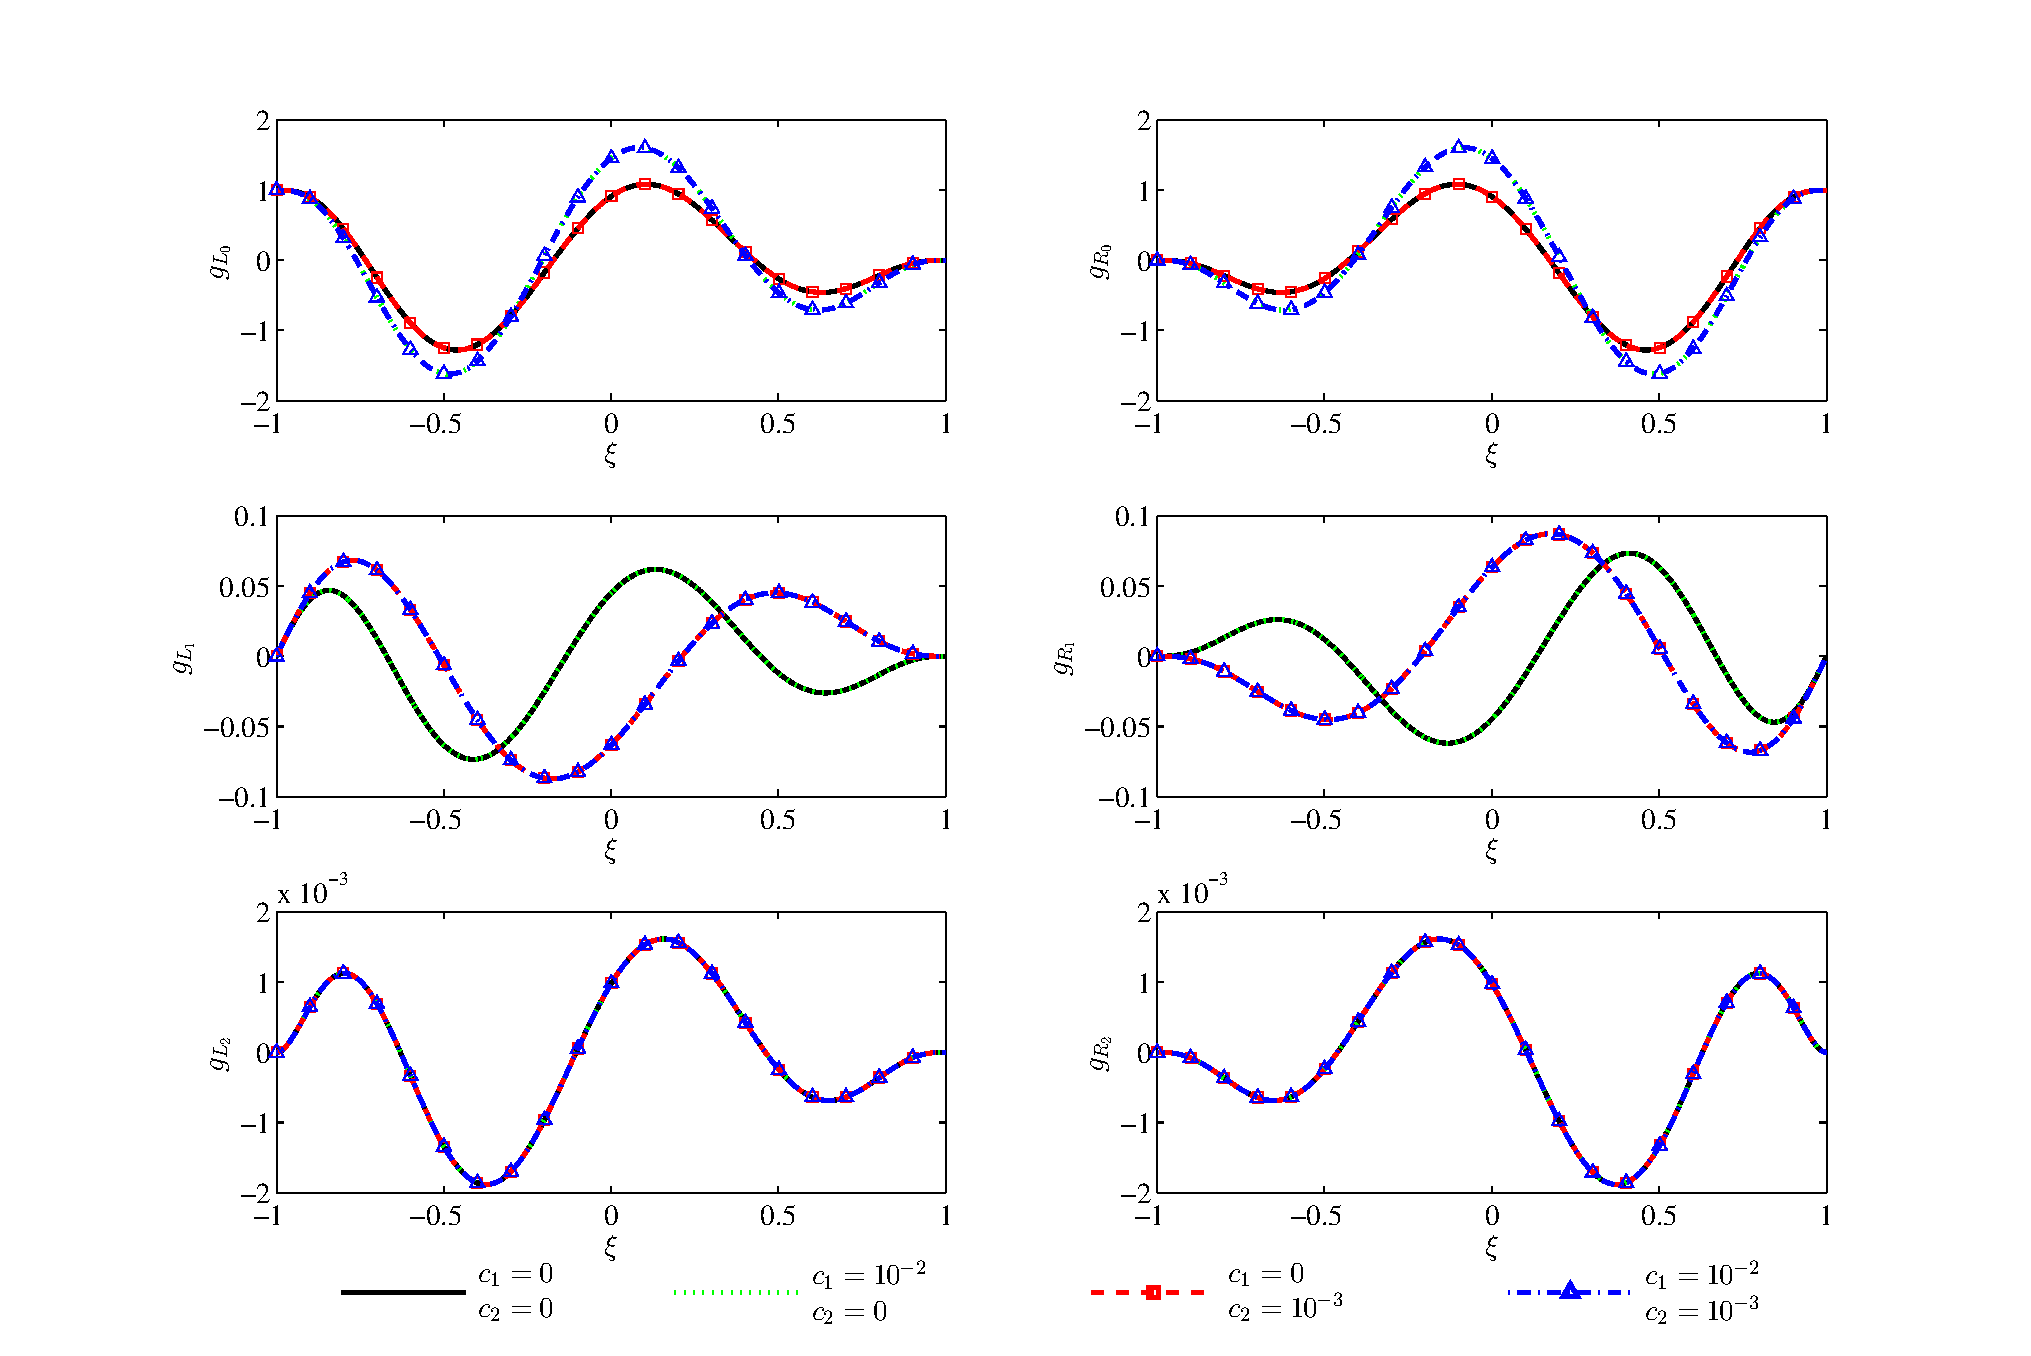
\includegraphics[width =1\textwidth,trim=\Ltrim cm 0cm \Rtrim cm 0cm]{\cmfrdir/Figures/Correction_funcs/C2FR} \caption{Left and right correction functions for the C2FR scheme with $P=3$, in which the zeroth, first, and second derivatives of the corrected flux are continuous} \label{fig:c2_corfunc} 
\end{figure}







\section{Numerical test cases}
\label{sec:num_cases}
In this section we present solutions to the linear advection equation using the C1FR scheme to show that it is stable and achieves the theoretical order of convergence of $P+1$ when the solution is discretized with an order $P$ polynomial. In addition, we present solutions to the linear advection-diffusion equation to demonstrate the ability to change the scheme's dispersion and dissipation properties while maintaining stability.

As can be seen from the derivation of the \gls{c1fr} scheme, the interface flux constants $\alpha_0$ and $\alpha_1$, the norm constants $c_0$ and $c_1$, and the location of the solution points at each element are variable. In this exposition, we will not modify the location of the solution points and use the standard zeroes of the Legendre polynomials. We note that the values of $c_1$ have a direct impact on the scheme's dispersion and dissipation, while --as expected-- the $\alpha_r$ values affect the dissipation only. A future rigorous Fourier analysis would reveal wiser choices for the $c_1$ parameter.


\subsection{Order of Accuracy of C1FR}
\subsubsection{Setup}

The 1-D experiments follow the procedure suggested by Vincent et al.~\cite{vincent2011insights} to estimate  a scheme's order of accuracy isolating interpolation errors. We solve the linear advection equation with advection speed of $a = 1$. The domain was $\Omega = [-10, 10]$ and was discretized in $n = 10, 15, 24, 38, 60$ equispaced elements of orders $P = 1,2,3$. The initial condition was a sine wave with wavenumber $k = 2\pi/20 \approx 0.63$. The advection speed was $1$ and fully upwinded fluxes $\alpha_0 = 0, \alpha_1 = 0$ in Eqn. \eqref{eq:ifluxdef}) were used. The boundary conditions were periodic. The simulation advanced using a fourth order \gls{rk} scheme with a time-step of order $10^{-3}$.

The initial condition was advected for a full domain length, using either standard nodal DG or \gls{c1fr}, and the resulting solution was taken as the reference solution $u_{ref}$. The wave was advected for a further full domain length to obtain the final solution $u_{final}$. The error was calculated by taking the L-2 norm of $u_{ref} - u_{final}$.

\subsubsection{Results and discussion}
Figures \ref{fig:adv_P1},\ref{fig:adv_P2}, and \ref{fig:adv_P3} show the rate of convergence of the solution and its derivative obtained by discretizing the solution wih polynomials of order $P = 1,2,3$, respectively. The slopes of the best fit lines are presented in each figure's caption.

\begin{figure}[h]
\centering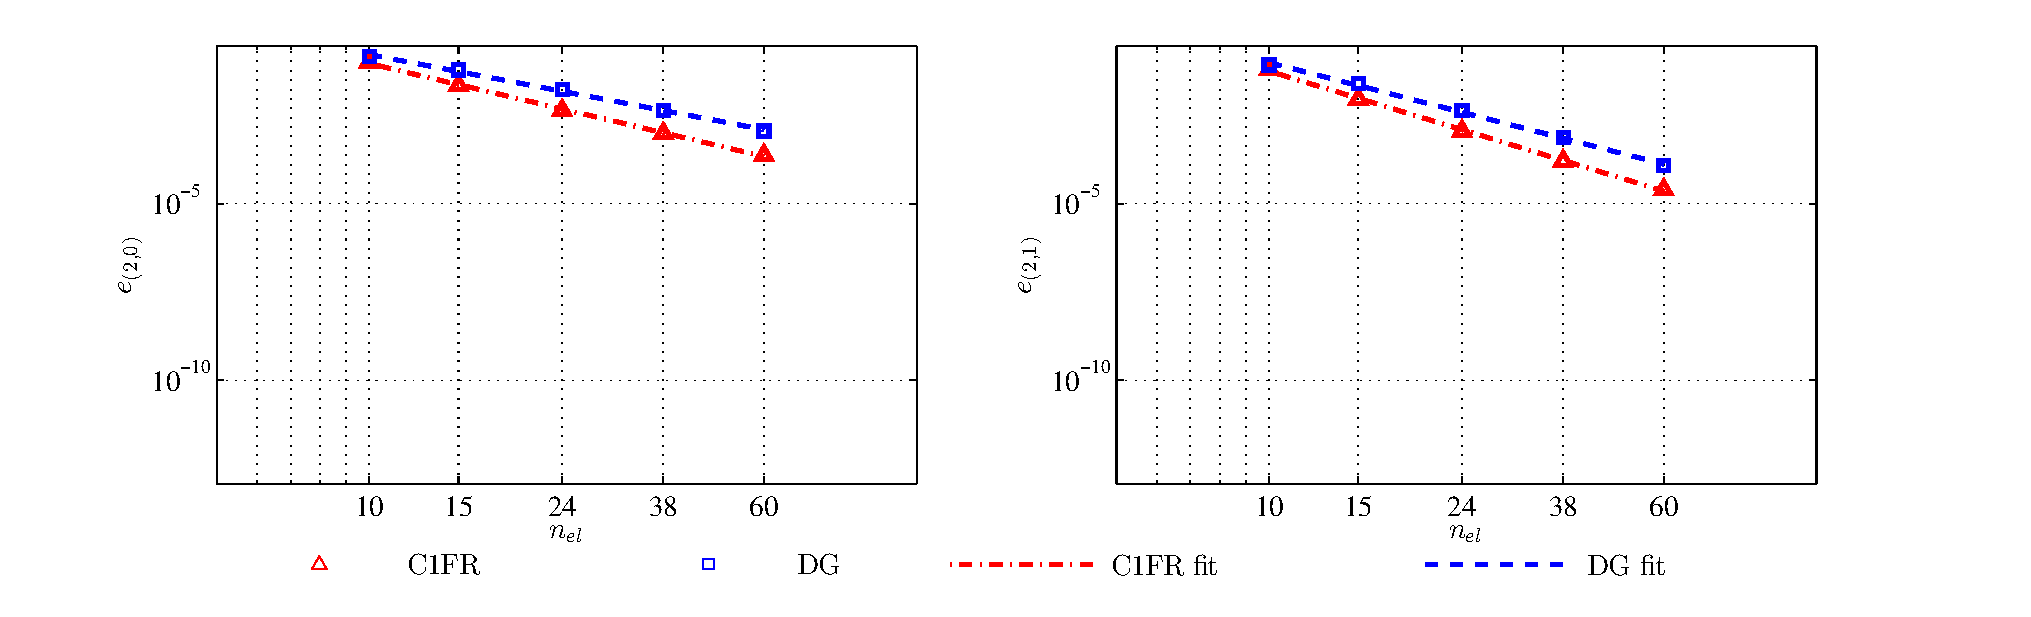
\includegraphics[width=1\textwidth,trim=\Ltrim cm 0cm \Rtrim cm 0cm]{\cmfrdir/Figures/Order_accuracy/P_1}
\caption{L-2 norm of error of advected sine wave and its derivative, $e_{(2,0)}$ and $e_{(2,1)}$ respectively, versus number of elements, for linear advection with polynomial discretization of order $P = 1$. Order of accuracy in solution: \gls{dg}: $2.728$, \gls{c1fr}: $3.374$. Order of accuracy in first derivative: \gls{dg}: $2.691$, \gls{c1fr}: $3.359$.}
\label{fig:adv_P1}
\end{figure}

\begin{figure}[h]
\centering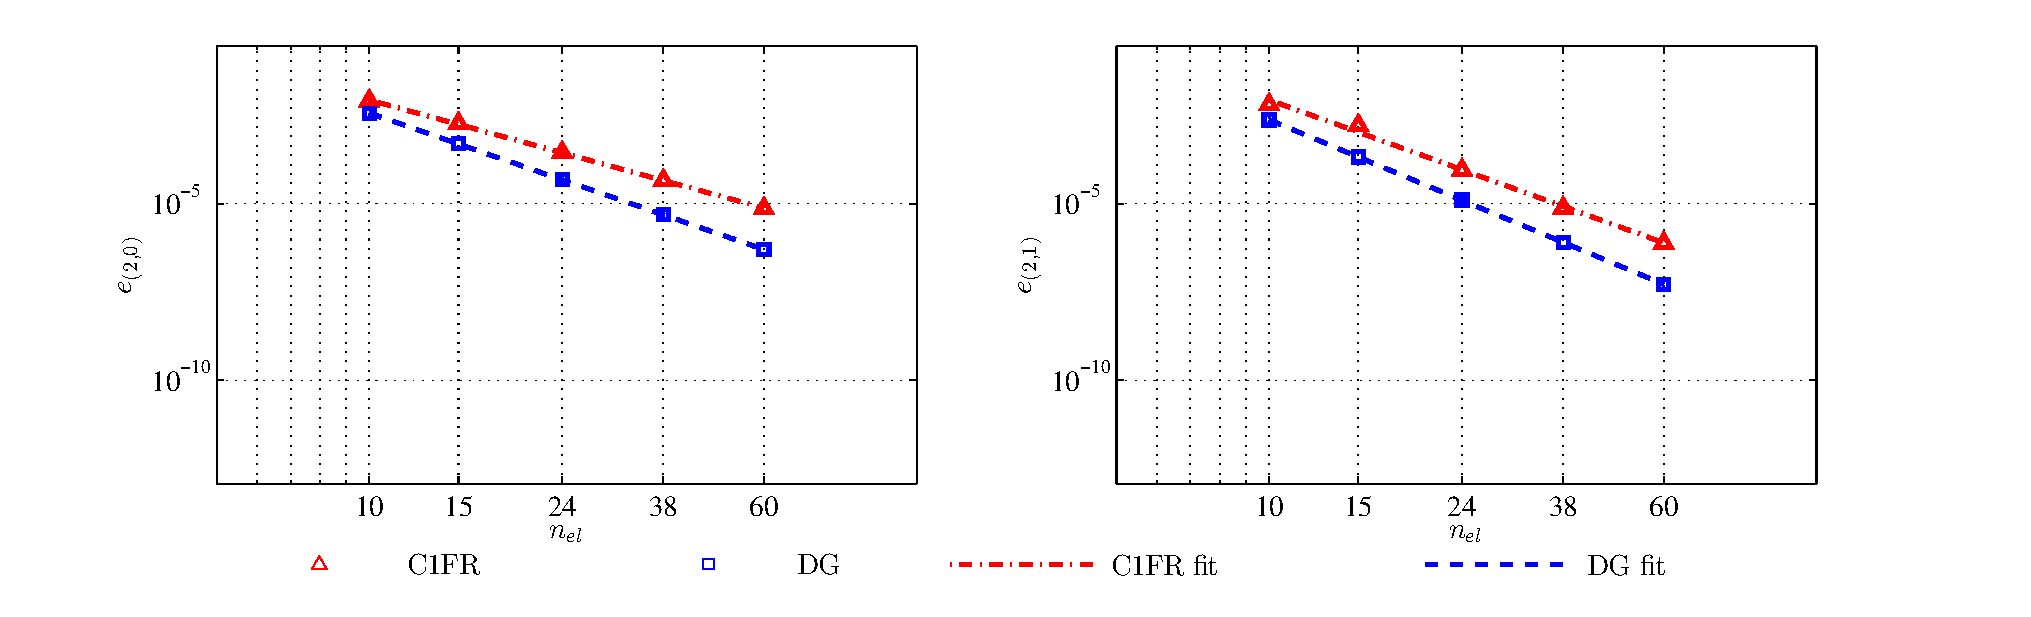
\includegraphics[width=1\textwidth,trim=\Ltrim cm 0cm \Rtrim cm 0cm]{\cmfrdir/Figures/Order_accuracy/P_2}
\caption{L-2 norm of error of advected sine wave and its derivative, $e_{(2,0)}$ and $e_{(2,1)}$ respectively, versus number of elements, for linear advection with polynomial discretization of order $P = 2$. Order of accuracy in solution: \gls{dg}: $4.960$, \gls{c1fr}:  $3.917$ . Order of accuracy in first derivative: \gls{dg}: $4.971$, \gls{c1fr}: $4.178$.}
\label{fig:adv_P2}
\end{figure}

\begin{figure}[h]
\centering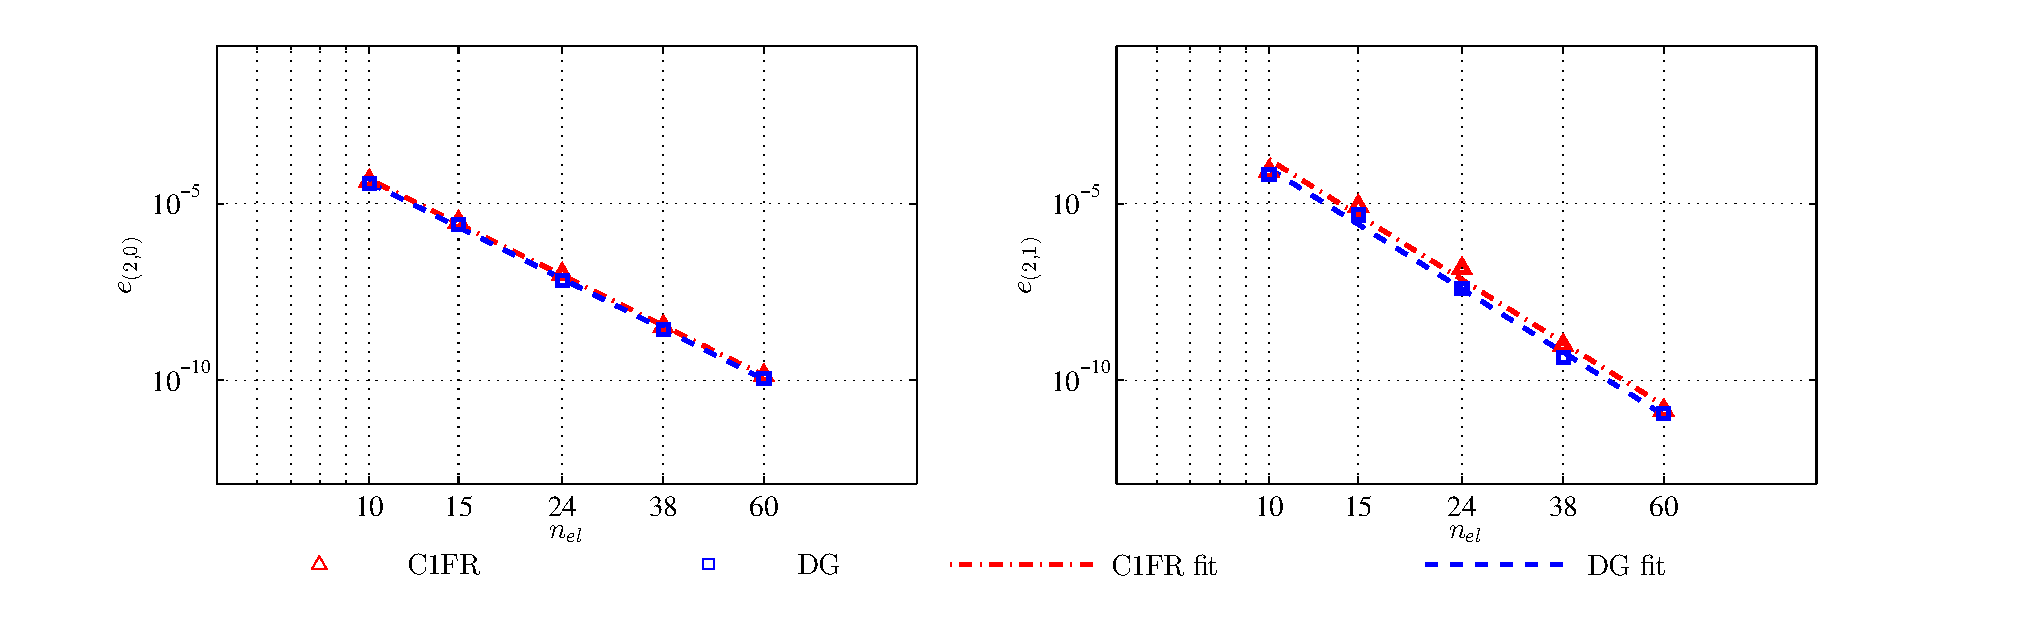
\includegraphics[width=1\textwidth,trim=\Ltrim cm 0cm \Rtrim cm 0cm]{\cmfrdir/Figures/Order_accuracy/P_3}
\caption{L-2 norm of error of advected sine wave and its derivative, $e_{(2,0)}$ and $e_{(2,1)}$ respectively, versus number of elements, for linear advection with polynomial discretization of order $P = 3$. Order of accuracy in solution: \gls{dg}: 7.119, \gls{c1fr}: 7.187. Order of accuracy in first derivative: \gls{dg}: 7.908, \gls{c1fr}: 7.882.}
\label{fig:adv_P3}
\end{figure}

The fact that we recover the expected nodal \gls{dg}'s $2P+1$ order of convergence found by Vincent et al. \cite{vincent2011insights} for $P = 1,2,3$ validates the experimental setup. It is interesting to note that \gls{c1fr} retains \gls{fr}'s even-odd order of convergence behavior: when $P$ is odd, the order of convergence is $2P+1$; while when $P$ is even, the order of convergence is $2P$.

This numerical experiment does not replace a von Neumann analysis, but does show that the scheme is stable, consistent, and maintains the desired order of accuracy. Although we would not expect the scheme to maintain super-convergence properties in real applications --as the interpolation errors are themselves of order $P+1$--, this experiment relieves worries about C1FR's introducing lower order errors.

\subsection{Advection-Diffusion Energy Preservation}
\label{sec:advDiff}
Motivated by the fact that in turbulent simulations the preservation of energy at different scales (or wavenumbers) is of paramount importance, we wanted to explore the potential benefit of having sets of families of stable numerical schemes with modifiable dispersion and dissipation properties.

By solving the linear advection-diffustion equation we are able to assess how much dissipation in different scales is due to numerics as opposed to the nature of the equation.

\subsubsection{Setup}

In these numerical experiments we solve the linear advection-diffusion equation using the C1FR and nodal DG schemes following the approach described by Huynh \cite{huynh2009reconstruction}. In essense, we re-write the diffusion-advection equation as a system of two first order \gls{pde}s as follows
\begin{equation}
\begin{split}
\dd{u}{t} + \dd{q}{x} = 0 \\
q - au + \kappa\dd{u}{x} = 0
\end{split}
\end{equation}

where $a$ is the advection speed, $\kappa$ is the diffusion coefficient, and $q$ is a dummy variable. The desired scheme is used to discretize the spatial differentiation.

In this section, we let $a = 1$, $\kappa = 10^{-2}$. The domain was $\Omega = [-10,10]$ and was discretized in $n = 20$ equispaced elements of polynomial order $P = 5$. The boundary conditions were periodic. The initial conditions were sine waves with low, medium, and high wavenumbers. The wavenumbers were chosen relative to the Nyquist limit of the discretization: 
\[k = \rho (P+1)\pi/h\]
 where $\rho$ is a non-dimensional constant, $P+1$ is the number of solution points in each element of polynomial degree $P$, and $h$ is the size of the element. Note that when $\rho = 1$, the Nyquist limit is reached exactly if the solution points are spaced evenly.

In our experiments, for the low wavenumber $\rho = 0.25$; medium wavenumber $\rho = 0.5$; high wavenumber $\rho = 0.75$. The fluxes were all fully upwinded and in the \gls{c1fr} scheme, $c_1 = -5\cdot10^{-3}$. The solution is advanced with a standard \gls{rk}4 time-stepping scheme. A \gls{cfl} of $0.3$ is used for both schemes. At each timestep, we calculate the square of the L-2 norm of the solution and its derivative, and compare it to the exact corresponding values. $||u||_{(2,m)} $ is the L-2 norm of the $m^{\text{th}}$ derivative of solution $u$.


\subsubsection{Results and discussion}
Fig. \ref{fig:low_wavenumber} shows that both schemes preserve the exact solution and derivative norms of the low wavenumber. On the other hand, \ref{fig:high_wavenumber} shows that both schemes suffer from aliasing and deviate significantly from the exact L-2 norms when the initial solution is a high wavenumber. \gls{c1fr} is somewhat closer to the exact values than nodal \gls{dg} both before and after the norms of the numerical solutions intersect the exact solution's L-2 norm.

Fig. \ref{fig:medium_wavenumber} presents a promising result. \gls{c1fr} preserves the correct L-2 norms of the solution while nodal \gls{dg}'s numerical dissipation affects the energy content of the wave. The L-2 norm of C1FR's solution derivative oscillates around the exact value, while nodal \gls{dg}'s oscillates with similar magnitude trending further below the exact values.


\begin{figure}[h]
\centering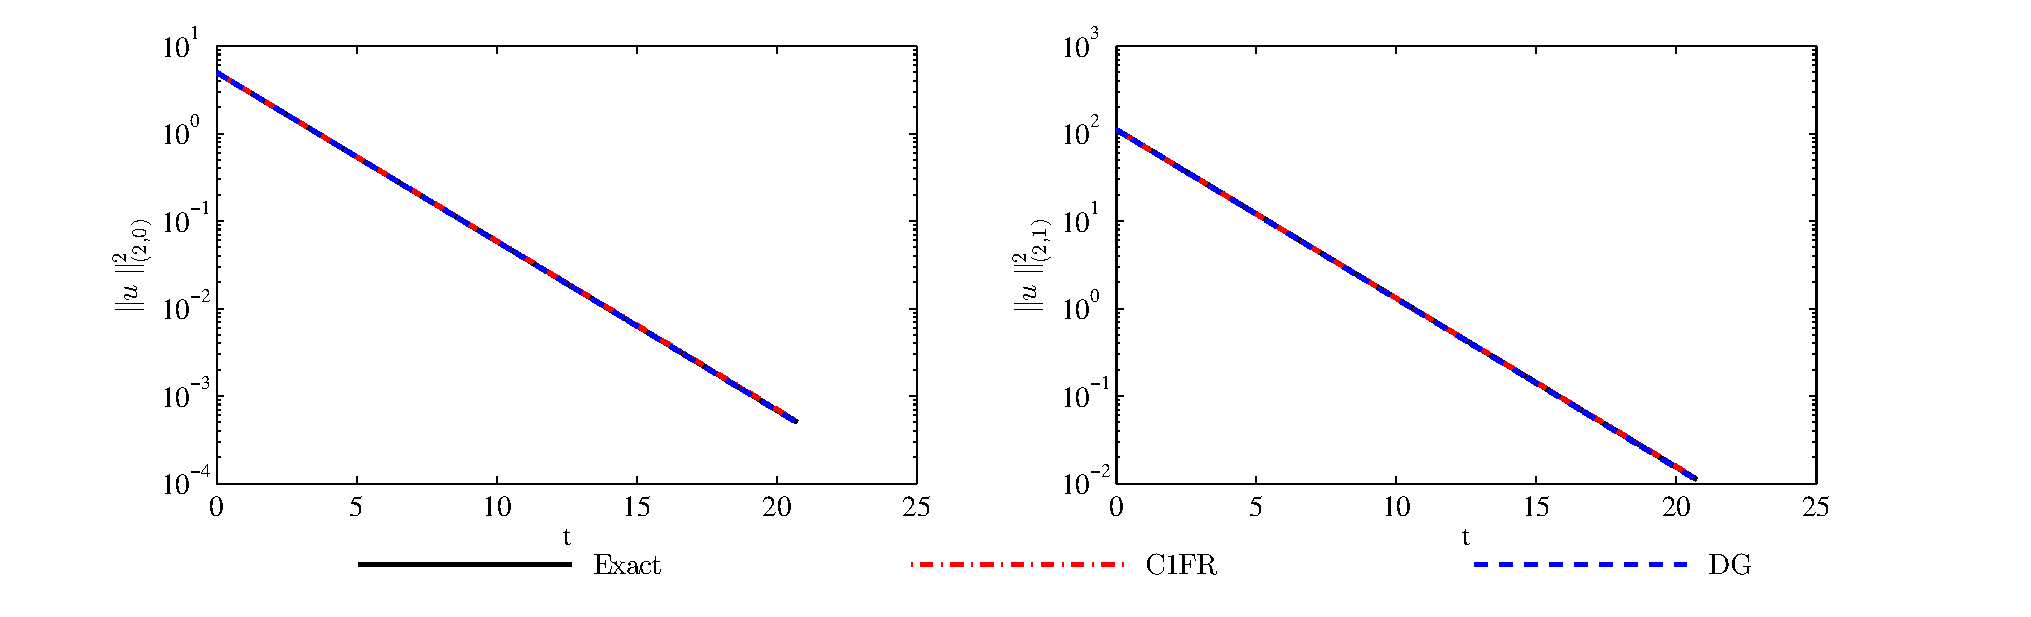
\includegraphics[width=1\textwidth,trim=\Ltrim cm 0cm \Rtrim cm 0cm]{\cmfrdir/Figures/Test_adv_diff/low_k}
\caption{Time history of norms of numerical solutions to the advection-diffusion equation and their first derivative. Initial condition is a sine wave with low wavenumber: $k = 0.25 (P+1)\pi/h$, $P = 3$, $h = 1$.}
\label{fig:low_wavenumber}
\end{figure}

\begin{figure}[h]
\centering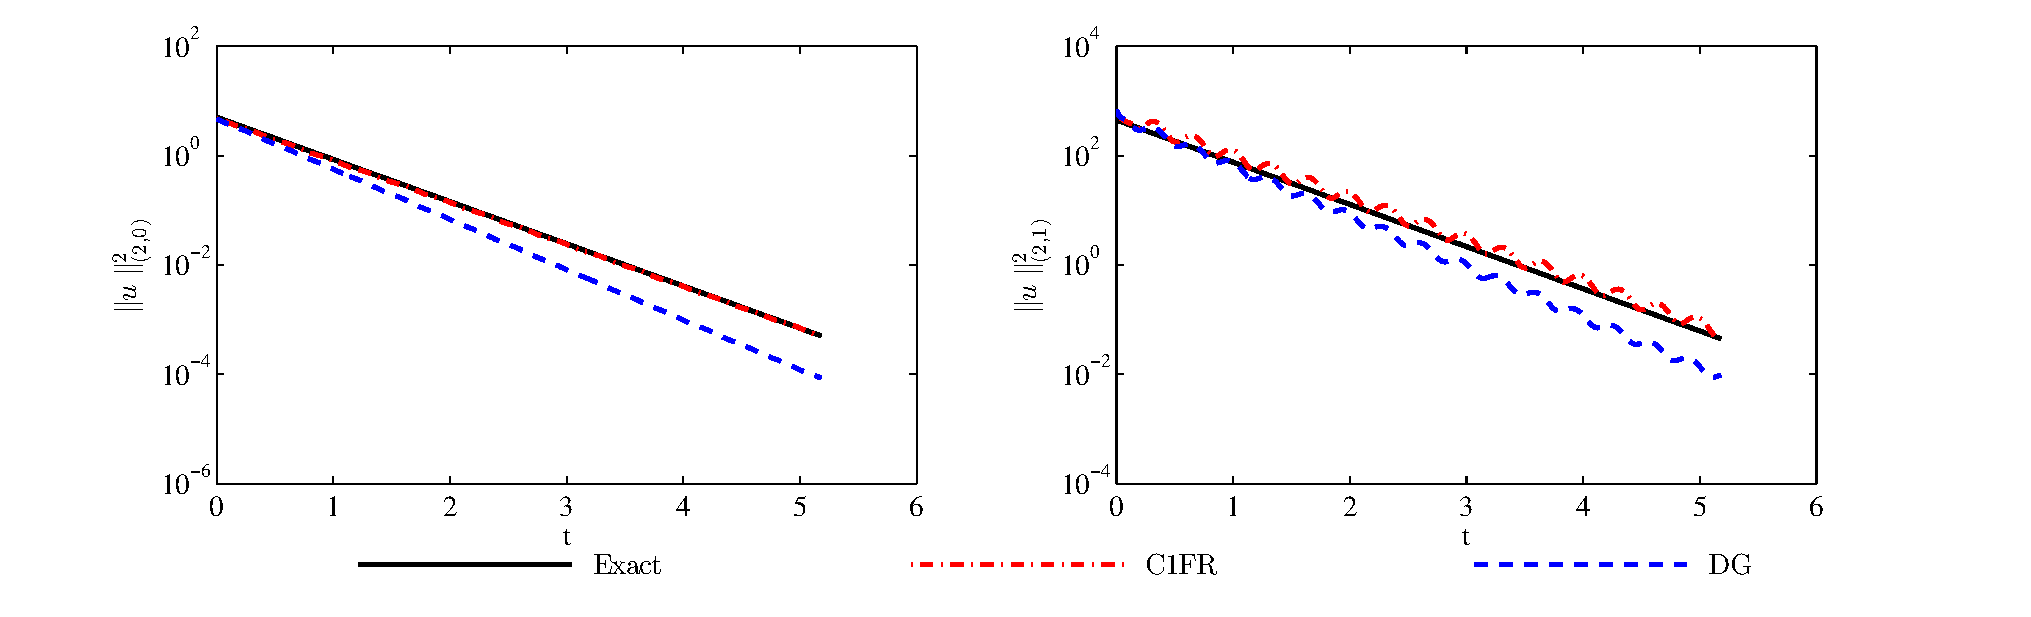
\includegraphics[width=1\textwidth,trim=\Ltrim cm 0cm \Rtrim cm 0cm]{\cmfrdir/Figures/Test_adv_diff/med_k}
\caption{Time history of norms of numerical solutions to the advection-diffusion equation and their first derivative. Initial condition is a sine wave with medium wavenumber: $k = 0.5 (P+1)\pi/h$, $P = 3$, $h = 1$.}
\label{fig:medium_wavenumber}
\end{figure}

\begin{figure}[h]
\centering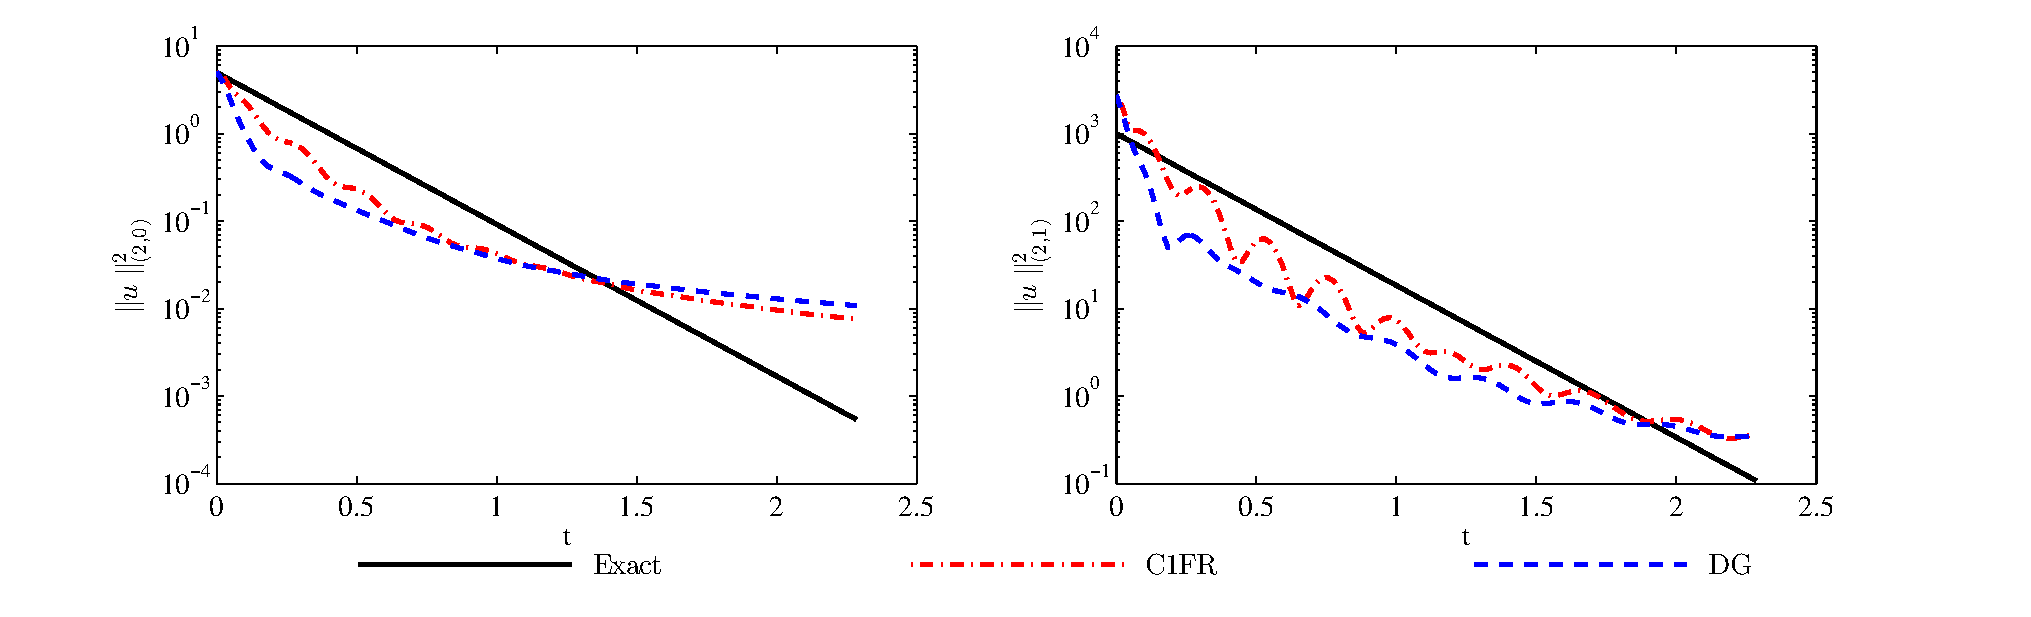
\includegraphics[width=1\textwidth,trim=\Ltrim cm 0cm \Rtrim cm 0cm]{\cmfrdir/Figures/Test_adv_diff/high_k}
\caption{Time history of norms of numerical solutions to the advection-diffusion equation and their first derivative. Initial condition is a sine wave with high wavenumber: $k = 0.75 (P+1)\pi/h$, $P = 3$, $h = 1$.}
\label{fig:high_wavenumber}
\end{figure}

%_ %_ %_ %_ %_ %_ %_ %_ %_ %_ %_ %_ %_ %_ %_ %_ %_ %
%\begin{figure}[h]
%\centering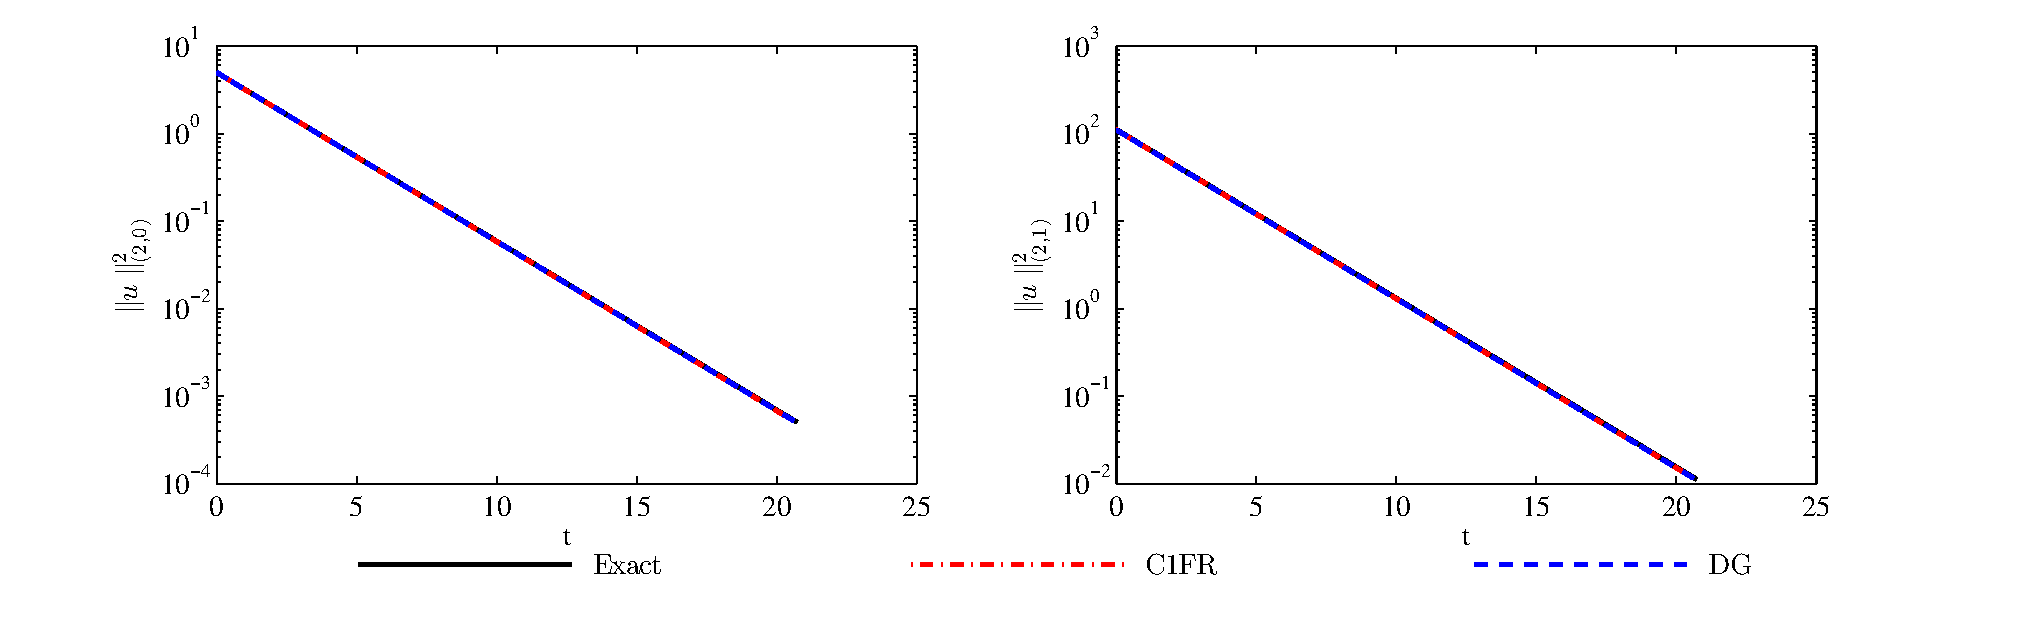
\includegraphics[width=1\textwidth,trim=\Ltrim cm 0cm \Rtrim cm 0cm]{Figures/Test_adv_diff/low_k_c_5e-3}
%\caption{Time history of norms of numerical solutions to the advection-diffusion equation and their first derivative. Initial condition is a sine wave with low wavenumber: $k = 0.25 (P+1)\pi/h$, $P = 3$, $h = 1$.}
%\label{fig:low_wavenumber2}
%\end{figure}
%
%\begin{figure}[h]
%\centering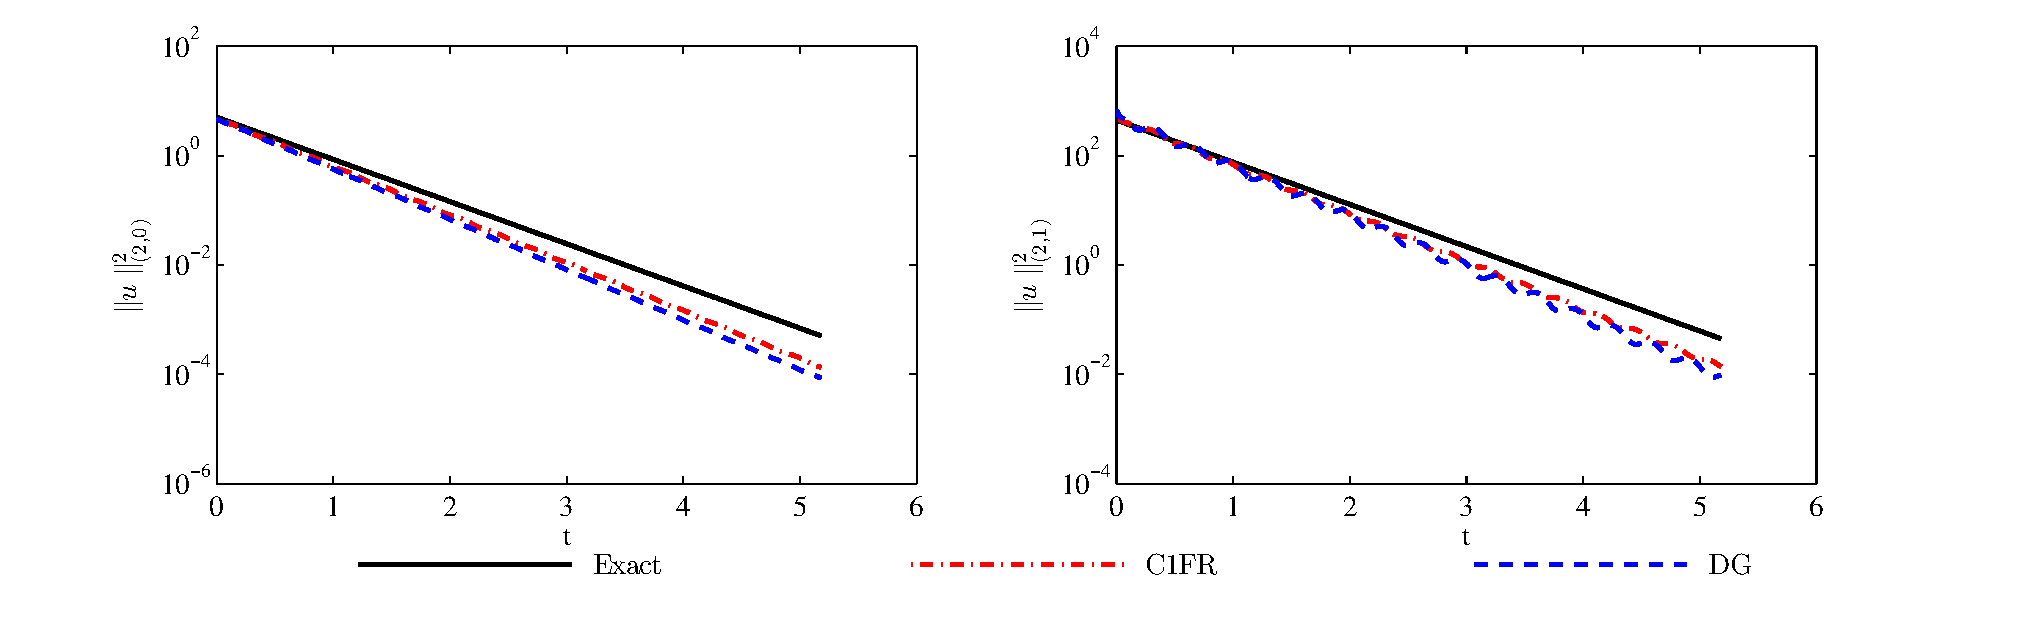
\includegraphics[width=1\textwidth,trim=\Ltrim cm 0cm \Rtrim cm 0cm]{Figures/Test_adv_diff/med_k_c_5e-3}
%\caption{Time history of norms of numerical solutions to the advection-diffusion equation and their first derivative. Initial condition is a sine wave with medium wavenumber: $k = 0.5 (P+1)\pi/h$, $P = 3$, $h = 1$.}
%\label{fig:medium_wavenumber2}
%\end{figure}
%
%\begin{figure}[h]
%\centering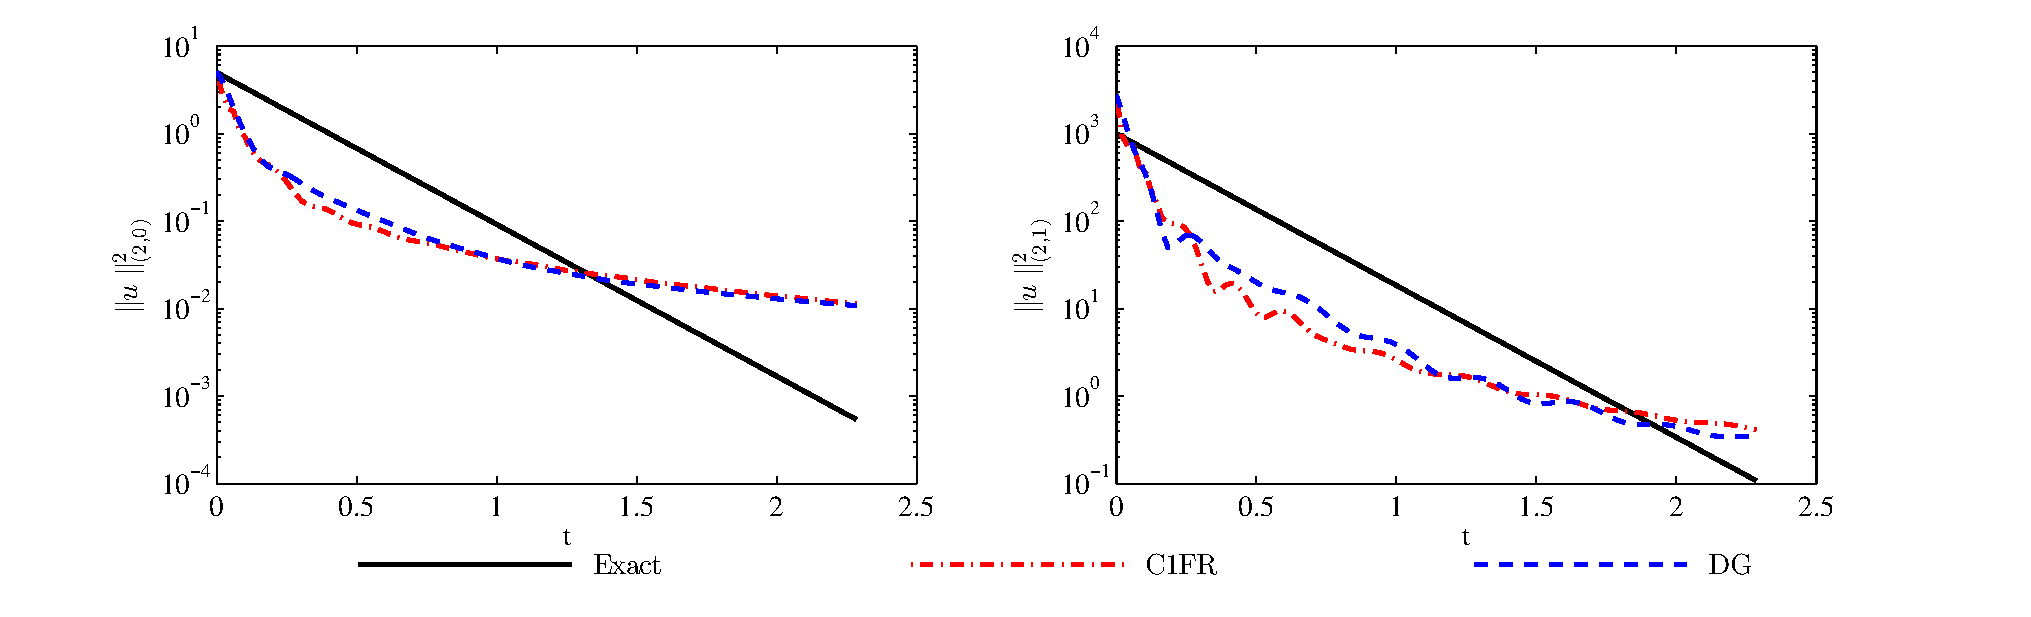
\includegraphics[width=1\textwidth,trim=\Ltrim cm 0cm \Rtrim cm 0cm]{Figures/Test_adv_diff/high_k_c_5e-3}
%\caption{Time history of norms of numerical solutions to the advection-diffusion equation and their first derivative. Initial condition is a sine wave with high wavenumber: $k = 0.75 (P+1)\pi/h$, $P = 3$, $h = 1$.}
%\label{fig:high_wavenumber2}
%\end{figure}

%_ %_ %_ %_ %_ %_ %_ %_ %_ %_ %_ %_ %_ %_ %_ %_ %_ %

%\begin{figure}
%\centering
%\subfigure[fig a]{\label{fig:high_wavenumber} 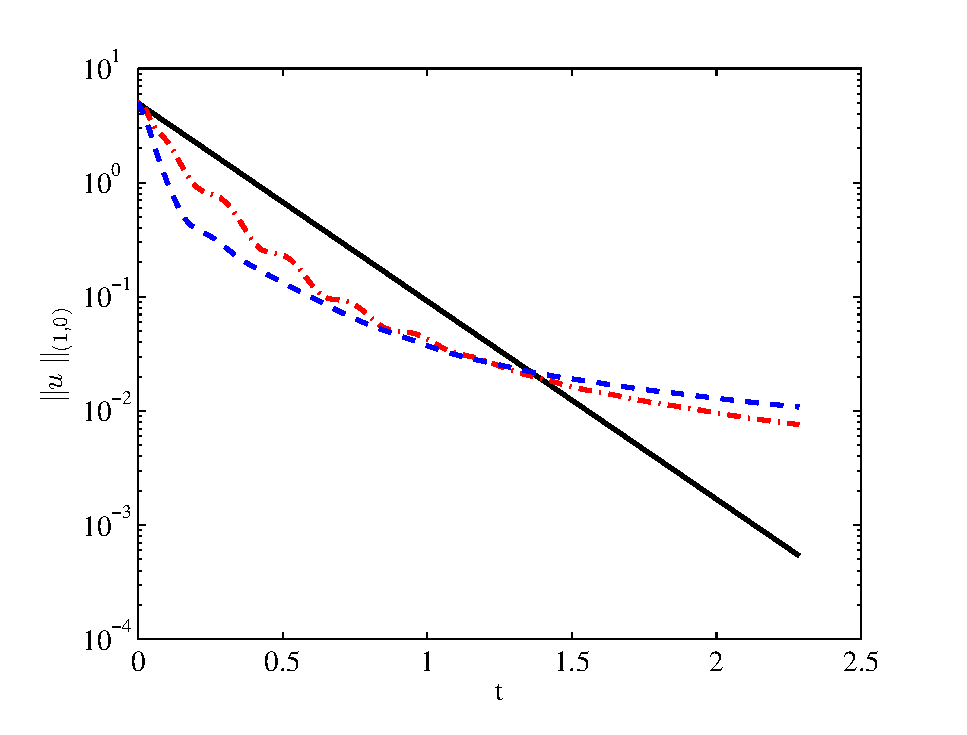
\includegraphics[width = .5\textwidth]{Figures/Test_adv_diff/eN0_high_k}
%\caption{energy history}}

%\end{subfig}
%\end{figure}



\section{Conclusions}

We have presented a natural extension of the \gls{fr} approach. The \gls{cmfr} schemes guarantee 1-D linear stability and introduce an arbitrary number of parameters that modify the scheme's dispersive and dissipative properties. The addition of these parameters require the representation of the reconstructed flux to be $p+1$ or higher, where $p$ is the order of the polynomial used to represent the conservative solution.

 We have shown the derivation of the \gls{c1fr} scheme, which has reconstructed fluxes continuous in the zeroth and first derivatives accross elements. This scheme, with a particular selection of its free parameter, was able to preserve the energy of an advected and diffused wave with a medium wavenumber better than the nodal \gls{dg} scheme. Certainly, this one example cannot be said to be generalizable. Nevertheless, it calls for a Von Neumann analysis to assess the impact of the free parameter on the scheme's properties. As the general \gls{cmfr} schemes have arbitrarily many such parameters, this analysis should be generalizable.

A major complication with the general \gls{cmfr} schemes is that the correction functions do depend on the element's Jacobian, so they are not as general and element-agnostic as those in the original \gls{fr} schemes. However, as shown by Allaneau~\cite{allaneau2011connections}, it is possible to formulate some \gls{fr} schemes as filtered \gls{dg} schemes without the need to find the correction functions explicitly. A similar analysis with the \gls{fr} schemes could yield element-dependent filtered \gls{dg} schemes whose properties can be understood or optimized in the \gls{cmfr} framework.

Future work should include numerical experiments in 2-D and 3-D using tensor product elements to assess the extent to which the stability guarantees in 1-D translate to other dimensions. In addition, it is still unclear if the degree of continuity of the corrected fluxes could be beneficial in the solution of high order partial differential equations.

%Borrow from the paper.
%
%\subsection{Introduction}
%
%\subsection{The $C^m$ Flux Reconstruction Approach}
%
%\subsection{Linear stability of $C^m$ continuous flux reconstruction}
%
%\subsection{Example of a CMFR scheme: C1FR}
%
%\subsection{Numerical experiments}
%\subsubsection{Verification of Order of Accuracy}
%\subsubsection{Advection-diffusion Energy Preservation}


\chapter{Local Fourier Spectral Filters}
%We propose the use of Local Fourier-Spectral (LFS) filters, developed originally for 1-D and 2-D tensor-product elements by Asthana and López-Morales [cite], as a parameter-free approach to stabilize high-order solutions. The LFS filters stabilize the solution, when needed, under all potential modes of failure. Their formulation adapts easily to Finite-Element-based spatial discretizations: the filter has a compact stencil, is not more expensive than a solution evaluation, and is discretization-agnostic. We present solutions to turbulent, transonic, and supersonic flows using the Flux Reconstruction approach, a high-order scheme heavily studied in the Aerospace Computing Laboratory. All solutions are obtained in coarse, unstructured grids using a medium-cost multi-GPU-powered workstation.
%
%\subsection{Introduction}
%Mention that author was seeking filters that could be posed as a matrix-vector multiplication with a local stencil. Inspiration came from paper by Lodato.
%
%\subsection{Non-linear stabilization of high-order Flux Reconstruction schemes}
%Present summary of paper by Asthana et al. and key results.
%
%\subsection{1-D and 2-D tensor product element filtering approach}
%Describe original approach by Asthana et al. to filtering: basis functions outside element of interest are defined as constants in 1-D, and extruded curves and constants in 2-D.
%
%\subsection{Extension to arbitrary elements}
%Describe how filtering matrix is composed of two submatrices: square matrix that modifies the spectrum (energetic content) of the solution, and rectangular matrix that ensures the filter is Essentially Local Extremum Diminishing.
%
%The formulation of this type of filter is agnostic to the type of element and basis functions used, and provides a framework to design new LFS.
%
%\subsection{Simulations}
%\subsubsection{1D}
%\subsubsection{2D}
%\subsubsection{3D}

\section{Introduction}
Low-order methods are ubiquitous in industry and academia. Regardless of the mesh quality and flow conditions, commercial \gls{cfd} packages output an answer. It is up to the informed user to decide if such answer is believable or accurate to her satisfaction. This is not so true of high-order methods: they are still sensitive to starting conditions, mesh quality, and the non-linearity of the flow, i.e. how high \gls{re} is. If any of these parameters is not chosen well, the simulation will halt prematurely and no result, not even a rough estimate, will be provided. Certainly, this is not acceptable in an industrial setting.

The \gls{lfs} filters being proposed in this chapter are an attempt at tackling the low robustness of high-order methods from the perspective of flow physics, rather than the classical frameworks of polynomial order reduction, artificial viscosity, or limiting. Very promising results have been shown by Asthana and the author~\cite{asthana2014} for 1D non-linear advection-diffusion problems and 2D inviscid high-\gls{ma} flows with quadrilateral, unstructured, coarse grids, and polynomial discretizations of up to order $8$. The present paper extends their formulation to arbitrary elements in arbitrary dimensions and shows results in high-\gls{re} flows without turbulence modeling.

It is well known that turbulent flows --which tend to be high-\gls{re}--, exhibit an energy cascade: the energy from large scales is transferred to smaller scales due to natural dissipation. In very crude terms, large vortices become ever smaller vortices until they reach dimensions proportional to the Kolmogorov length-scale~\cite{kolmogorov1962refinement}. This phenomenon is well captured by the \gls{ns} equations. Hence, a good \gls{ns} solver would see large scales become ever smaller. In general, low-order methods in grids not created for \gls{dns} introduce enough numerical dissipation that the ever shrinking scales are dissipated before they become aliased (or under-sampled).

We postulate that it is precisely this very natural energy cascade which is de-stabilizing high-order numerical methods. Because high-order methods introduce little numerical dissipation, the ever shrinking scales may not be dissipated before they become aliased: they re-appear as larger scales that, naturally, become smaller later on. This vicious cycle introduces non-physical energy into the flow until the simulation is de-stabilized. Thus, removing the small scales before they become aliased would, in theory, stabilize the solution.

\gls{lfs} filters target scales relative to the element size, as the filtering operation happens in the reference element. The smaller the element, the smaller the scale being filtered. In addition, the filters help satisfy boundary conditions. The  results presented here show that the \gls{lfs} filters can  stabilize not only high-$\Re$ flows but also moderate-$\Ma$ and low-$\Ma$ flows in coarse grids, which opens the door to using the filters as pre-conditioners or in multigrid cycles. All simulations being presented ran from start to finish without intervention.

Many stabilization schemes created for high-order methods have focused on shock-capturing. A concise review of the shock-capturing literature can be seen in Section 3.4 in~\cite{vincent2011facilitating}. An \gls{av}-based shock capturing approach that has gained popularity because of its ease of implementation and increase of robustness was suggested by Persson and Peraire~\cite{persson2006sub}. A similar approach for high-$\Re$ flows with turbulence modeling has been proposed by Nguyen et al.~\cite{nguyen2007rans}. Lodato~\cite{lodato2014structural} has used filtering in the formulation of \gls{sgs} models for \gls{les} with high-order \gls{sd} schemes. His work inspired the formulation of the filters presented here. A stabilization strategy based on optimization was suggested by Guba et al.~\cite{guba2014optimization} shows great promise. A limiter-based stabilization strategy easily implemented in \gls{dg}-type methods was proposed by Kuzmin~\cite{kuzmin2004high} and Lv et al.~\cite{lv2015entropy}.

The main reason we decided to find a stabilization strategy that could be posed as a matrix multiplication and requires a very local stencil arises from the fact that \gls{hf} performs best on \gls{gpu}s. \gls{gpu}s require a low-communication, highly-parallel implementation with organized memory accesses and homogeneous computations. Implementation of \gls{av} would have required elements adjacent to each other to share information about the \gls{av} that each requires, leading to inevitable additional inter-element communication.

 Section \ref{sec:frmethod} presented a general description of the \gls{fr} method. Section \ref{sec:extension_multiple_dimensions} showed how this scheme relies on matrix multiplications and, hence, a filter that costs two small matrix multiplications per element is ideal for \gls{fr}. Section \ref{sec:lfsfilter} describes the properties being sought in the \gls{lfs} filters and the mechanics of their implementation. Section \ref{sec:visualization} provides visualizations of the filters and their effects on a polynomial solution. Section \ref{sec:results} presents the results of 2D simulations, in unstructured coarse grids, of flows where \gls{re}$= 1e6$. This \gls{re} number was selected because of the availability of experimental data for the case of the circular cylinder and \gls{hf} had not been run at these \gls{re} numbers. In addition, Section \ref{sec:filteringEffects} shows results that isolate the effects of filtering from the effects of coarsening a grid or changing the spatial order of accuracy to demonstrate that \gls{lfs} filters preserve element-wise spectral properties.


\vspace{.20in}



\vspace{.20in}

\section{Local Fourier Spectral Filters}
\label{sec:lfsfilter}

\subsection{Desired Properties}
\label{sec:lfs_properties}
When designing the \gls{lfs} Filters presented in this paper, we considered the following properties as desirable:
\begin{enumerate}[1. ]
\item The filter should have spectral interpretation so there is control over the physical scales being smoothed
\item \label{item:local_stencil} The filtering operation must have a local stencil: only interior and boundary solution values can be used to filter the solution in the interior of the element
\item \label{item:filt_bc}The filter should preserve boundary conditions
\item \label{item:filt_bi}Filtering the solution at the interior points should be influenced by the solution values at the element's boundary
\item \label{item:influence}The influence of a boundary point on the internal point being filtered should be inversely proportional to the distance between them
\item To limit computational cost, the filter should be applied in the reference domain and involve matrix-vector multiplications exclusively

\item \label{item:generalizability}Filtering strategy should be generalizable to any type of element in unstructured grids

In the early stages of the filter design, we noted that Properties \ref{item:filt_bc} and \ref{item:filt_bi} could be overly stringent, so we re-phrased them as the following, more relaxed condition:

\item \label{item:coplanar}If solution values at the boundary lie on a hyperplane in the space of spatial coordinates and solution values, the filtering operation should bring the internal solution values closer to such plane. In other words, if the solution values at the boundaries can be determined from a linear function of their location, the filter should bring the internal solution values closer to satisfying such linear function.
\end{enumerate}



Condition \ref{item:coplanar} may not allow a filtered solution to satisfy the boundary conditions always. Nevertheless, in the limit of infinite mesh refinement the solutions at the boundary of every element will be coplanar, even in the presence of shocks in the \gls{ns}  equations. Hence, Condition \ref{item:coplanar} satisfies conditions \ref{item:filt_bc} and \ref{item:filt_bi} asimptotically. This re-formulation was inspired by the \gls{eled}  property of the \gls{jst}  scheme\cite{jameson1981numerical} for finite volume methods. Whether or not (some) \gls{lfs} filters satisfy \gls{eled}  properties shall be left for a future study.

%At this point it is important to note the main difference between the filters being proposed here and the commonly used modal filters\cite{kanevsky2006idempotent}. Modal filters are not influenced by the values of the solution at the boundary points. Therefore, if an element is experiencing aliasing, a modal filter will not necessarily ``nudge" the internal solution values towards continuity with its neighbors. In addition, in the limit of mesh refinement, modal filtering might not enforce an element's boundary conditions.

\subsection{Mechanics of \gls{lfs} Filters}

The core idea of the \gls{lfs} filtering technique is that the solution is filtered with a matrix whose entries depend on the element interface values, the basis functions of the solution, and a selected Fourier filtering kernel.

Suppose we wish to filter the scalar field $v$ inside an arbitrary element. This field could be density, momentum in a specific direction, or energy. We can represent $v$, as usual, as a weighted sum of basis functions.
\begin{equation}
\label{eqn:polyexp}
v(\bxi) = \sum^{N_s}_{i=1} v_i \phi_i(\bxi),
\end{equation}
where $v_i$ is the \ith weight, $\bxi$ is a vector of coordinates in a reference domain, and $\phi_i(\bxi)$ is the \ith basis function.

The key component of the \gls{lfs} technique is that the Fourier filtering operation over the element is approximated at each internal point $i$ with coordinates $\bxi_i$. Suppose we wish to use filtering kernel $G(\bxi)$ to filter $v(\bxi)$, then the filtered value at internal point $i$ becomes
\begin{equation}
\label{eqn:convolution}
\begin{split}
\bar{v}_j &= (G \ast v)(\bxi_j)\\
&= \int_{\mathbb{R}^d} G(\bxi_j - \bxi)v(\bxi)d\bxi\\
&= \int_{\mathbb{R}^d} G(\bxi_j - \bxi)\l(\sum^{N_s}_{i=1} v_i \phi_i(\bxi)\r)d\bxi\\
&= \sum^{N_s}_{i=1}v_i\int_{\mathbb{R}^d} G(\bxi_j - \bxi)  \phi_i(\bxi)d\bxi,\\
\end{split}
\end{equation}

where $\Omega$ is the entire problem domain, not just the element domain, $N_s$ is the number of solution points, and the overbar means the quantity is filtered. Filtering over the entire domain would be computationally expensive, but would certainly smoothen the solution field and can be done while maintaining the order of accuracy of the underlying numerical scheme\cite{mirzaee2012efficient,steffen2008investigation,walfisch2009one}. In order to use only a local (element-wise) stencil, it is possible to break the integration as follows
\begin{equation}
\label{eqn:brokenint}
\int_{\mathbb{R}^d} G(\bxi_j - \bxi)  \phi_i(\bxi)d\bxi = \int_{\Omega_n} G(\bxi_j - \bxi)  \phi_i(\bxi)d\bxi + \int_{\mathbb{R}^d \backslash \Omega_n} G(\bxi_j - \bxi)  \phi_i(\bxi)d\bxi,
\end{equation}
where $\Omega_n$ is the domain of element $n$ (where the $\phi_i$ values are known) and $\Omega \backslash \Omega_n$ is the complement of $\Omega_n$ in $\Omega$. As $G$ and $\phi_i$ are defined in $\Omega_n$, it is possible to calculate the first integral in Equation \eqref{eqn:brokenint} analytically or via an adaptive quadrature algorithm like \texttt{quanc8}~\cite{forsythe1977computer}.

A design choice arises in defining $\phi_i$ in the domain $\Omega \backslash \Omega_n$. Asthana et al.~\cite{asthana2014} initially decided to let $\phi_i$ equal a constant in 1D elements, and a combination of constant and polynomial in quadrilaterals. Non-tensor-product elements became problematic for this kind of formulation. This paper presents a more generic filter design method based on the desired properties in Section \ref{sec:lfs_properties}.

Let us describe the mechanics of the two components of the integral in Equation \eqref{eqn:brokenint} in a subsection each. We can call the filter associated with the term $\int_{\Omega_n} G(\bxi_j - \bxi)  \phi_i(\bxi)d\bxi$ ``Internal Filtering Component" and the filter associated with the term $\int_{\mathbb{R}^d \backslash \Omega_n} G(\bxi_j - \bxi)  \phi_i(\bxi)d\bxi$ ``Boundary Filtering Component".

The filtering operation being sought follows this format
\begin{equation}
\label{eqn:filter_form}
\vec{\bar{v}} = \alpha\mat{T}\vec{v} + (1-\alpha)\mat{B}\vec{v^*},
\end{equation}
where $\mat{T}$ is the internal filtering component, as it acts on the solution at internal points $\vec{v}$, and $\mat{B}$ is the boundary filtering component, as it acts on the solution at boundary points $\vec{v^*}$, and $\alpha$ is a scalar between $0$ and $1$ that determines the relative influence the internal and boundary components have on the internal solution values.

\subsection{Internal Filtering Component}
There are two steps to the creation of the internal filtering component $\mat{T}$. First we create the filtering matrix with the spectral interpretation, and then we normalize it so if the quantity being filtered is a constant, the filter preserves the constant.
\subsubsection{Matrix formation}
It can be seen from the last line in Equation \eqref{eqn:convolution} that finding the vector of solution values filtered with the internal component can be posed as a matrix-vector multiplication:
\begin{equation*}
\label{eq:internal_matrix}
\begin{bmatrix}
\bar{v}_1 \\
\bar{v}_2 \\
\vdots\\
\bar{v}_{N_s} \\
\end{bmatrix} = 
\begin{bmatrix}
\int_{\Omega_n} G(\bxi_1 - \bxi)  \phi_1(\bxi)d\bxi &
\int_{\Omega_n} G(\bxi_1 - \bxi)  \phi_2(\bxi)d\bxi &
\cdots &
\int_{\Omega_n} G(\bxi_1 - \bxi)  \phi_{N_s}(\bxi)d\bxi\\
\int_{\Omega_n} G(\bxi_2 - \bxi)  \phi_1(\bxi)d\bxi &
\int_{\Omega_n} G(\bxi_2 - \bxi)  \phi_2(\bxi)d\bxi &
\cdots &
\int_{\Omega_n} G(\bxi_2 - \bxi)  \phi_{N_s}(\bxi)d\bxi\\
\vdots & \vdots & \ddots & \vdots\\
\int_{\Omega_n} G(\bxi_{N_s} - \bxi)  \phi_1(\bxi)d\bxi &
\int_{\Omega_n} G(\bxi_{N_s} - \bxi)  \phi_2(\bxi)d\bxi &
\cdots &
\int_{\Omega_n} G(\bxi_{N_s} - \bxi)  \phi_{N_s}(\bxi)d\bxi
\end{bmatrix}
\begin{bmatrix}
v_1 \\
v_2 \\
\vdots\\
v_{N_s} \\
\end{bmatrix}.
\end{equation*}

More compactly,
\begin{equation}
\label{eqn:filtmat}
\vec{\bar{v}} = \mat{F}\vec{v}
\end{equation}
we use over-arrow to denote column vectors.
Interesting choices for $G(\bxi)$ depend on a desired wavenumber threshold $h$:

\begin{enumerate}[I.]
\item Gaussian function:
$$
G(\bxi) = h \exp{(h||\bxi||)},
$$
where $||\bxi||$ is a measure of the length of $\bxi$.
\item \label{item:multi_ind_func}Multidimensional indicator function:
$$
G(\bxi) = h\mathrm{I}_{[0,1]}(h||\bxi||),
$$
where $\mathrm{I}_{[0,1]}(x) = 1 \text{ if } 0\le x\le 1$, and $0$ otherwise.
\item \label{item:sharp_spectral}Multidimensional sharp-spectral function:
$$
G(\bxi) = h||\bxi||^{-n/2}
J_{n/2}(h||\bxi||),
$$
where $J_\alpha$ is a Bessel function of the first kind and $n$ is the number of dimensions of $\bxi$.
\end{enumerate}

In these functions, the larger the value of $h$, the thinner the filter is in physical space, so the fewer wavenumbers it dampens. Note that as $h \rightarrow \infty$, $\mat{F}_{ij}  \rightarrow \phi_j(\bxi_i)$, so $\vec{\bar{v}} \rightarrow \vec{{v}}$. The integrals in Equation \eqref{eq:internal_matrix} can be evaluated to arbitrary accuracy with \texttt{quanc8}~\cite{forsythe1977computer} in a pre-processing stage.

\subsubsection{Enforcing Conservation of a Constant Quantity}
The requirement to preserve a constant can be posed in an equation as
\begin{align}
\bar{v}_i = \sum^{N_s}_{j = 1} \mat{F}_{ij} v_{\text{const}} = v_{\text{const}},
\end{align}
where $v_{\text{const}}$ is a constant scalar. As a result, each row of $\mat{F}$ must satisfy
\begin{align}
\sum^{N_s}_{j = 1} \mat{F}_{ij} = 1,
\end{align}
where $i = 1,\dots,N_s$.
This constraint can be enforced by dividing each row of $\mat{F}$ with the total sum of the row. More explicitly,
\begin{align}
{\mat{T}}_{ij} = \frac{\mat{F}_{ij}}{\sum^{N_s}_{k = 1} \mat{F}_{ik}},
\end{align}
where the normalized matrix ${\mat{T}}$ is the internal filtering component in Equation \eqref{eqn:filter_form}.

\subsubsection{Integration Domain}

The normalization of the matrix introduces a bias. As the integration is being performed in some reference domain $\Omega_n$, the integral $\int_{\Omega_n} G(\bxi_i - \bxi)  \phi_j(\bxi)d\bxi$ will tend to have a greater value when $\bxi_i$ is well inside the reference element. This is more evident when using the multidimensional indicator function (shown in \ref{item:multi_ind_func}) as the filtering kernel.

To ameliorate this bias, we have selected to perform the integration in a reference domain that is symmetric. With this precaution all integrals related to points close to a domain edge have a similar magnitude, and thus the filtering operation does not favor points close to some arbitrary edge over the others.

Figure \ref{fig:domain_example} illustrates the potential introduction of bias in triangular elements that use a right triangle as a reference element.

\begin{figure*}

\subfloat[Equilateral triangle domain\label{fig:equi_tri_domain}]{%
      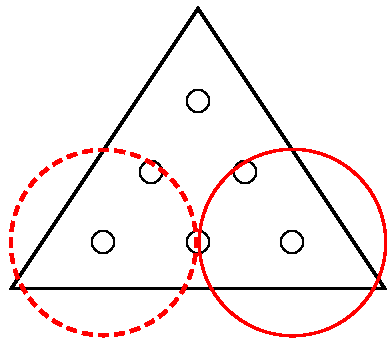
\includegraphics[width=0.45\textwidth]{\lfsdir/figs/equi_tri.pdf}
    }
    \hfill
    \subfloat[Right triangle domain\label{fig:right_tri_domain}]{%
          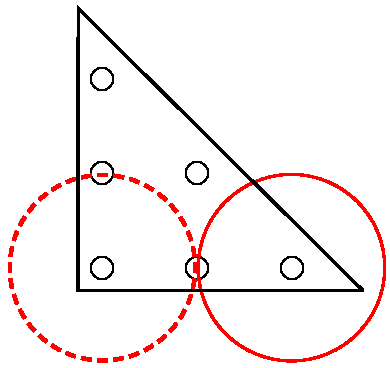
\includegraphics[width=0.45\textwidth]{\lfsdir/figs/right_tri.pdf}
        }
\caption{Using the same filter width in two different domains introduces different bias. The small, solid circles represent the location of solution points. The large circles represent the filter width acting on two specific internal points in two different domains. Integration is being performed in the area encompassed by the solid, straight lines.}
\label{fig:domain_example}

\end{figure*}

In practice, the basis functions $\phi_j(\bxi)$ may be defined in non-symmetrical elements. To simplify the evaluation of the integral, the definition of the norm in the filtering kernel $G(\bxi)$ can be modified so the curve drawn by $||\bxi -\bxi_0|| = 1$ in the non-symmetric reference element would map to a circle in a symmetric reference element.

In the case of a triangle, the basis functions are defined in a right triangle with vertices $[-1,-1], [1,-1],[-1,1]$.

By defining the norm in this right triangle as follows
\begin{equation}
\label{eqn:rect_norm}
||\bxi||^2_{rt} = \bxi_1^2 + \bxi_2^2 + \bxi_1\bxi_2,
\end{equation}
$||\bxi -\bxi_0||_{rt} = 1$ maps to a circle in the equilateral triangle with vertices $[-1,-1],[1,-1],[0,\sqrt{3}-1]$. Figure \ref{fig:mapping} sketches this mapping. $||\cdot||_{rt}$ is the norm defined in the right triangle.


\begin{figure}\centering
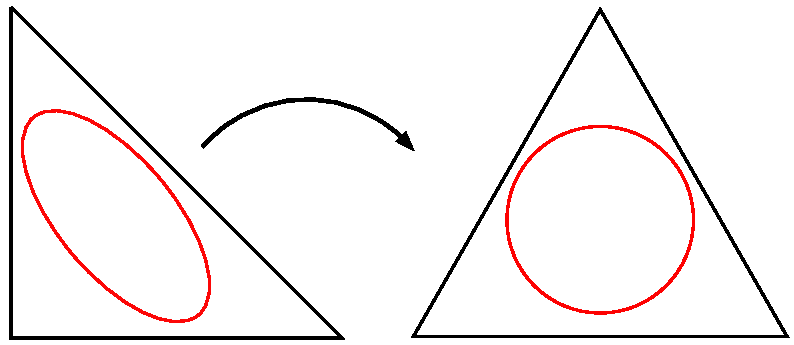
\includegraphics[width = 0.75\textwidth]{\lfsdir/figs/mapping.pdf}
\caption{Sketch of ellipsis $||\bxi -\bxi_0||_{rt} = 1$ defined in the right triangle domain maps to a circle in the equilateral triangle domain}
\label{fig:mapping}
\end{figure}

\subsection{Boundary Filtering Component}

Formulating the influence of boundary solution values on internal solution values as a matrix is not so straightforward. The approach being suggested here is based on some reasonable desired properties, but some choices are arbitrary. 

The creation of this matrix proceeds as follows: place the boundary points and the internal points in a symmetric domain, select an ``influence" function with as many unknowns as dimensions, find values for these unknowns such that Condition \ref{item:coplanar} is satisfied, and create the boundary filtering component.

\subsubsection{Ensuring Boundary Filtering Component Preserves Linearity of the Solution at the Boundary (Condition \ref{item:coplanar})}
In this sub-section, we seek to form matrix $\mat{B}$ in Equation \ref{eqn:filter_form}. In this analysis, we assume that $\alpha = 0$ in Equation \ref{eqn:filter_form} so we can isolate $\mat{B}$'s properties from those of $\mat{T}$.

The preservation of linearity can be posed in the following way. Assume that values $\vec{v^*}$ at the boundaries are linear in space. More explicitly, for each boundary point $i = 1,\dots,N_f$
\begin{equation}
v^*_i = {\bxi^*_i}^\mathrm{T}\vec{a} + b,
\end{equation}
where $v^*_i$ is the solution at the \ith boundary point, $\bxi_i^*$ are the coordinates of such boundary point, $\vec{a}$ is a vector of constant coefficients, and $b$ is a constant scalar. In vector notation, we are assuming

\begin{equation}
\label{eq:linear}
\vec{v^*} = \underline{\bxi^*}^\mathrm{T}\vec{a} + \vec{b^*},
\end{equation}
where $\vec{b^*} = b\mathbbm{1}_{[N_f \mathrm{x} 1]}$ and $\underline{\bxi^*}^\mathrm{T}$ is a matrix of dimensions $N_f$ by $N_d$ --number of dimensions.

To satisfy Condition \ref{item:coplanar}, we seek a matrix $\mat{B}$ such that, when $\vec{v^*}$ satisfies Equation \ref{eq:linear},
\begin{equation}
\vec{\bar{v}} = \mat{B}\vec{v^*} = \underline{\bxi}^\mathrm{T} \vec{a} + \vec{b},
\end{equation}
where $\vec{b} = b\mathbbm{1}_{[N_s \mathrm{x} 1]}$ and $\underline{\bxi}^\mathrm{T}$ is a matrix of dimensions $N_s$ by $N_d$. The \ith row of $\underline{\bxi}^\mathrm{T}$ is ${\bxi_i}^\mathrm{T}$, the coordinates of the \ith internal point.

Therefore, we seek a matrix $\mat{B}$ such that
\begin{equation}
\mat{B}\l(\underline{\bxi^*}^\mathrm{T}\vec{a} + \vec{b^*}\r) = \underline{\bxi}^\mathrm{T} \vec{a} + \vec{b}.
\end{equation}

As a result, for general $ \underline{\bxi^*}^\mathrm{T}$, $\underline{\bxi}^\mathrm{T} $, and $\vec{a}$,
\begin{align}
\mat{B}\underline{\bxi^*}^\mathrm{T} = \underline{\bxi}^\mathrm{T}  \hspace{1cm} &\text{and} \hspace{1cm} \mat{B}\vec{b^*} = \vec{b}\\
\label{eqn:Bconditions}\implies \hspace{1cm} \sum_{j=1}^{N_f}\mat{B}_{ij}\xi^*_{jd} = \xi_{id} \hspace{1cm} &\text{and} \hspace{1cm} \sum_{j = 1}^{N_f} \mat{B}_{ij} = 1
\end{align}
for all $i = 1,\dots,N_s$ and $d = 1,\dots,N_d$. Where $\xi^*_{jd}$ is the $d^\text{th}$ coordinate of the $j^\text{th}$ boundary point, and $\xi_{id}$ is the $d^\text{th}$ coordinate of the $i^\text{th}$ internal point.

Equation \ref{eqn:Bconditions} introduces $N_s (N_d + 1)$ constraints for $N_sN_f$ unkonwns in $\mat{B}$. Each row in $\mat{B}$ needs to satisfy $N_d+1$ equations. Table \ref{tab:conds_unknowns} shows the number of equations and unknowns for specific elements assuming that the solution whithin each is represented by a polynomial of degree $p\ge0$.

\newcommand{\len}{0.6cm}

    \begin{table}

    \cellspacebottomlimit=5pt
    \cellspacetoplimit=5pt
%      \begin{center}
        \newlength{\oldtabcolsep}                 % keep track of old \tabcolsep
        \setlength{\oldtabcolsep}{\tabcolsep}     % 6.0pt
        \setlength{\tabcolsep}{0pt}               % so coloring doesn't run off
                                                  % ends of the table
        \renewcommand{\arraystretch}{2}         % because math expressions
                                                  % almost run into each other
%        \begin{tabular}{Sl<{\hspace{2cm}}l<{\hspace{\oldtabcolsep}}l}  
\hspace{-2cm}
\begin{tabular}{l <{\hspace{\len}}c <{\hspace{0.2cm}} c <{\hspace{0.2cm}}c<{\hspace{\len}} c<{\hspace{\len}} c<{\hspace{\len}} c }

          \toprule
Element type & $N_s$& $N_d$ & $N_f$ & \specialcell[b]{\# of Equations:\\ $N_s (N_d + 1)$} & \specialcell[b]{\# of Unkowns:\\$N_sN_f$} \\
          \specialrule{\lightrulewidth}{0pt}{0pt} % so row-coloring aligns

Line & $p+1$ & $1$ & $2$ &$2(p+1)$ & $2(p+1)$\\

Triangle & $\frac{1}{2}(p+1)\cdot(p+2)$ & $2 $ & $3(p+1)$ & $\frac{3}{2}(p+1)\cdot(p+2)$ & $\frac{3}{2}(p+1)^2\cdot(p+2)$\\
Quadrilateral & $(p+1)^2$ & $2$ & $4(p+1)$ & $3(p+1)^2$ & $4(p+1)^3$\\
Tetrahedron & \specialcell[t]{$\frac{1}{6}(p+1)\cdot(p+2)$\\$\cdot(p+3)$} & $3 $ & $4\frac{1}{2}(p+1)\cdot(p+2)$ & \specialcell[t]{$\frac{2}{3}(p+1)\cdot(p+2)$\\$\cdot(p+3)$} & \specialcell[t]{$\frac{1}{3}(p+1)^2\cdot(p+2)^2$\\$\cdot(p+3)$}\\
Pyramid & \specialcell[t]{$\frac{1}{6}(p+1)\cdot(p+2)$\\$\cdot(2p+3)$} & $3 $ & \specialcell[t]{$4\frac{1}{2}(p+1)\cdot(p+2)$\\$ + (p+1)^2$}  & \specialcell[t]{$\frac{2}{3}(p+1)\cdot(p+2)$\\$\cdot(2p+3)$} & \specialcell[t]{$\frac{1}{6}(p+1)^2\cdot(p+2)$\\$\cdot(2p+3)\cdot(3p+5)$}\\
Prism & $\frac{1}{2}(p+1)^2\cdot(p+2)$ & $3 $ & \specialcell[t]{$2\frac{1}{2}(p+1)\cdot(p+2)$\\$ + 3(p+1)^2$} & $2(p+1)^2\cdot(p+2)$ & \specialcell[t]{$\frac{1}{2}(p+1)^3\cdot(p+2)$\\$\cdot(4p+5)$}\\
Hexahedron & $(p+1)^3$ & $3 $ & $6(p+1)^2$ & $4(p+1)^3$ & $6(p+1)^5$\\
          \bottomrule
        \end{tabular}
%      \end{center}
      \caption{Number of internal points $N_s$, number of boundary points $N_f$, and number of equations and unknowns in matrix $\mat{B}$ for each type of element, assuming the solution is being discretized with a polynomial of degree $p$}
      \label{tab:conds_unknowns}

    \end{table}

All elements, except for the line element, have matrices $\mat{B}$ with more unknowns than equations. This calls for a reduction of the number of unknowns in a strategic way. This is achieved by invoking Condition \ref{item:influence}: the farther away a boundary point is from an internal point, the less influential it should be.

\subsubsection{Ensuring Influence of Boundary Points on Internal Points is Inversely Proportional to their Distance (Condition \ref{item:influence})}
Given this requirement and Equation \eqref{eqn:Bconditions}, a reasonable design choice for each entry in $\mat{B}$ is:
\begin{equation}
\label{eq:bij_unmodified}
\mat{B}_{ij} = \frac{g_i\l(||\bxi_i - \bxi_j^*|| \r)^{-1}}{\sum\limits_{k=1}^{N_f}g_i\l(||\bxi_i - \bxi_k^*|| \r)^{-1}},
\end{equation}
where $\bxi_i$ is the location of the \ith internal point, $\bxi_j^*$ is the location of the \jth boundary point, and $g_i(\cdot)$ is a monotonically increasing function and $g_i(0) = 0$. The norm $||\cdot||$ is ideally defined in a symmetric element, or a reformulation of a norm in an non-symmetric element as in Equation \eqref{eqn:rect_norm}. We note that the requirement that $\sum_{j = 1}^{N_f} \mat{B}_{ij} = 1$ is immediately satisfied regardless of the exact form of $g_i(\cdot)$.

To avoid dividing by zero when $||\bxi_i - \bxi_j^*|| = 0$, we can recast Equation \eqref{eq:bij_unmodified} as
\begin{equation}
\label{eq:bij_def}
\mat{B}_{ij} = \frac{1}{1 + g_i\l(||\bxi_i - \bxi_j^*|| \r)\sum\limits_{\substack{k=1\\k \ne j}}^{N_f}g_i\l(||\bxi_i - \bxi_k^*|| \r)^{-1}}.
\end{equation}
This definition of $\mat{B}$ is now too stringent, so it is not clear if the conditions in Equation \eqref{eqn:Bconditions} are satisfied for any selection of $g_i(\cdot)$. Each row in $\mat{B}$ has $N_d$ equations left to satisfy.

By introducing $N_d$ unknowns in the definition of $g_i(\cdot)$ we can expect to satisfy the remaining $N_d$ equations per row. A choice made here is to let
\begin{equation}
\label{eqn:g_def}
g_i(x) = \sum_{d = 1}^{N_d} a_{id} x^d,
\end{equation}
where $x$ is a scalar, and $a_{id}$ are the unknowns to be found in each row $i$.

To find the values of $a_{id}$, a regular non-linear minimization function can be invoked. In this paper, we used the downhill simplex method by Nelder and Mead~\cite{nelder1965simplex}. The implementation in C++ was adapted from Jia \cite{simplexCode}. The function being minimized for each row $i$ of $\mat{B}$ is
\begin{equation}
J_i(a_{i1},\dots,a_{1N_d})=\sum_{d=1}^{N_d}\l(\sum_{j=1}^{N_f}\mat{B}_{ij}\xi^*_{jd} - \xi_{id}\r)^2,
\end{equation}
where $J_i$ is the cost function to be minimized related to row $i$. In occasions, the minimum of $J$ does not reach machine zero. However, as it will be shown in the case of triangles, $\mat{B}$ still behaves as desired.


\vspace{.30in}

\section{Visualization of the \gls{lfs} Filters in Triangular Elements}
\label{sec:visualization}
In this section we present visualizations of the effect of the \gls{lfs} filters on a polynomial solution of degree $5$ in a reference triangle.

In the plots that follow, the internal and boundary points are located as shown in Figure \ref{fig:tri_points}.
\epstopdfsetup{update}
\begin{figure}
\centering
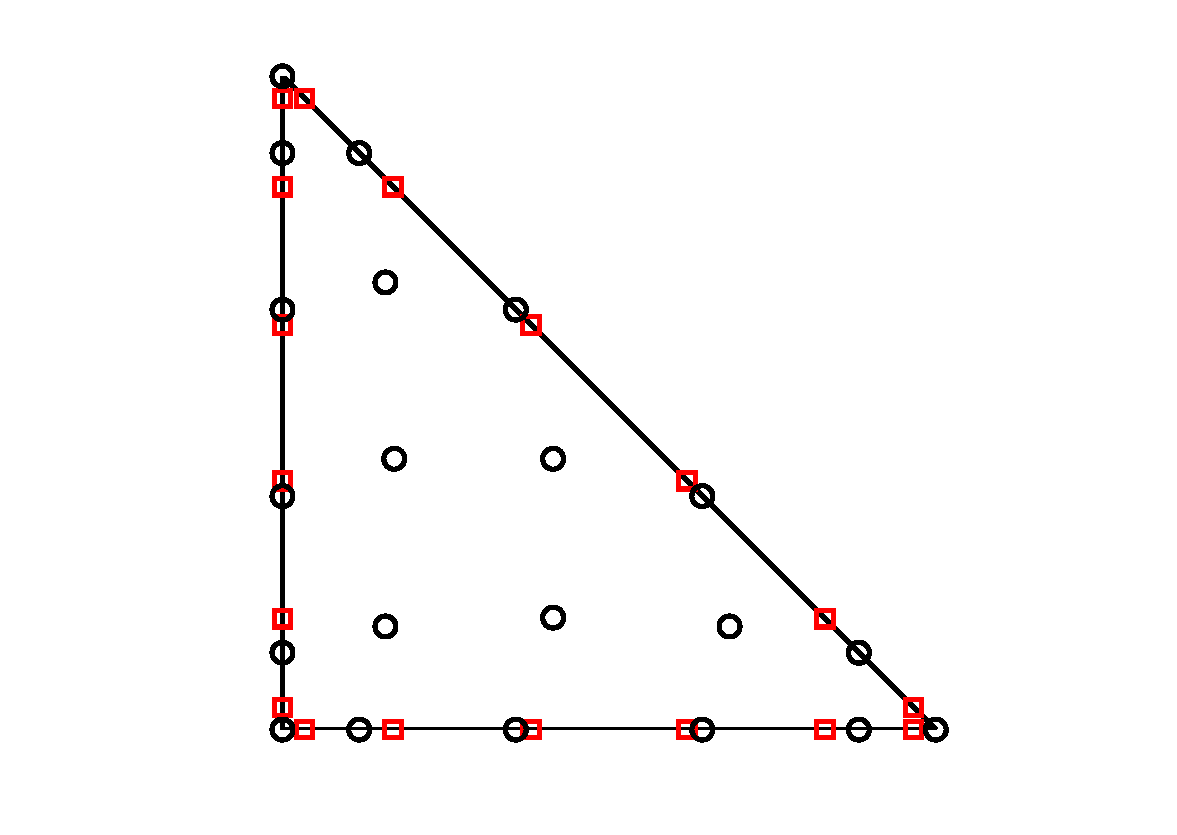
\includegraphics[width = 0.5\textwidth]{\lfsdir/figs/right_triangle_point_locations.eps}
\caption{Internal and boundary points in the reference triangular domain when solution is represented with polynomial of degree $5$ ($p=5$). Black circles represent the internal points. Red squares represent the boundary points.}
\label{fig:tri_points}
\end{figure}

\subsection{Internal Filtering Components}
To illustrate the effect of the internal filtering component, let us filter a solution using matrix $\mat{T}$ exclusively. Figure \ref{fig:internal_filt} shows the result of filtering using a width of $h=10$ in the 2-D sharp-spectral filtering kernel \eqref{item:sharp_spectral} with the modified norm \eqref{eqn:rect_norm}.
\begin{figure}
\centering
\includegraphics[width = 0.5\textwidth]{\lfsdir/figs/internal_effect.eps}
\caption{Solution values after filtering with internal component exclusively, $\vec{\bar{v}} = \mat{T}\vec{v}$, where  ${v_i} = \sin{(k\xi_{i1})} + \cos{(k\xi_{i2})} $, where $k=500$. Hollow black circles show the unfiltered solution at the interior points, transparent colored surface is the polynomial representation of the unfiltered solution, filled black circles show the filtered values of the solution at the interior points, and the meshed surface shows the polynomial representation of the filtered solution.}
\label{fig:internal_filt}
\end{figure}

It can be seen that the polynomial representation of the filtered values is smoother than the polynomial representation of the unfiltered values while maintaining the general shape and curvature.



\subsection{Boundary Filtering Components}
To illustrate the effect of the boundary filtering component, let us filter a solution using matrix $\mat{B}$ exclusively. Figure \ref{fig:boundary_effect} shows the result of filtering. Because only $\mat{B}$ is acting on the solution, the unfiltered values of the solution at the internal points are not plotted. 

We have made all the values of the solution at the boundaries co-planar to illustrate how effectively Condition \ref{item:coplanar} is satisfied. The operation of filtering with $\mat{B}$ does bring the filtered solution closer to a plane if the boundary values are co-planar.

\begin{figure}
\centering
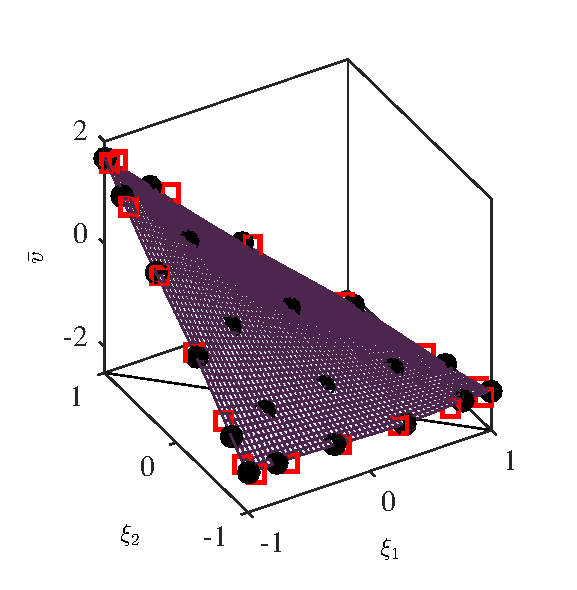
\includegraphics[width = 0.5\textwidth]{\lfsdir/figs/boundary_effect.eps}
\caption{Solution values after filtering with boundary component exclusively, $\vec{\bar{v}} = \mat{B}\vec{v^*}$, where  $\vec{v^*} = a\vec{\xi^*_1} + b\vec{\xi^*_2} + c$ for some constants $a,b,c$. Red squares show the values of the solution at the boundaries, filled black circles show the filtered values of the solution at the interior points, and the meshed surface shows the polynomial representation of the solution.} 
\label{fig:boundary_effect}
\end{figure}

Figure \ref{fig:boundary_effect_oscillatory} illustrates how the boundary filtering component would behave in the case the boundary values are not coplanar. It is interesting to note that close to the corner $(\xi_1,\xi_2) = (-1,1)$, two boundary points with different values are close to an internal point. The value  of the filtered solution close to those boundary points assumes a value that is close to the average of the two.

The polynomial interpolation of the filtered interior values shows that the closer an interior point is to a boundary point, the more it will be influenced by such boundary point. This causes the filtered values close to the boundaries to get closer to the boundary values. This suggests that the boundary filtering component does in fact help in bringing the solution closer to satisfying the boundary conditions while diminishing oscillations within the element.

\begin{figure}
\centering
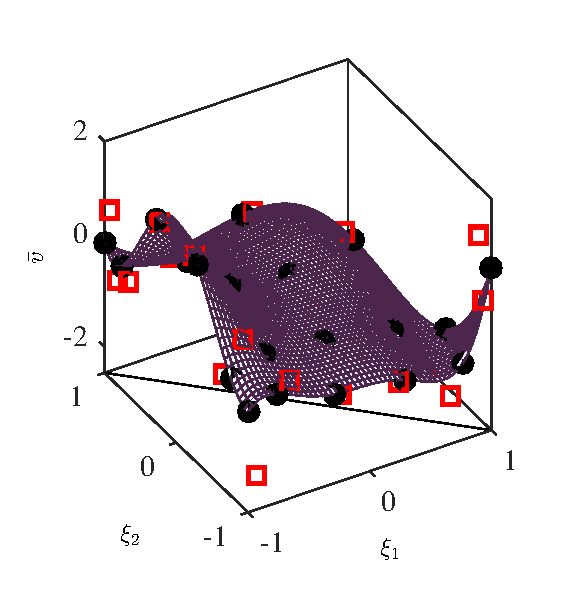
\includegraphics[width = 0.5\textwidth]{\lfsdir/figs/boundary_effect_oscillatory.eps}
\caption{Solution values after filtering with boundary component exclusively, $\vec{\bar{v}} = \mat{B}\vec{v^*}$, where   ${v_i^*} = \sin{(k\xi^*_{i1})} + \cos{(k\xi^*_{i2})} $, $k=500$. Red squares show the values of the solution at the boundaries, filled black circles show the filtered values of the solution at the interior points, and the meshed surface shows the polynomial representation of the solution.} 
\label{fig:boundary_effect_oscillatory}
\end{figure}

\subsection{Filtered Solutions}
No filtering component is used solely by itself. The factor $\alpha$ in Equation \ref{eqn:filter_form} determines how much weight to give to each component. Figure \ref{fig:filtered_solutions} illustrates the effect of the boundary values on a fully filtered solution, when $\alpha = 0.8$.

The internal filtering component reduces oscillations, while the boundary filtering component brings the interior values closer to the boundary values. By placing the boundary values on different planes, this effect becomes more evident.

\begin{figure*}
\hspace{-1cm}
\subfloat[$\beta = -0.75$\label{fig:filt_neg}]{%
\includegraphics[width=0.5\textwidth]{\lfsdir/figs/filter_tilt_neg.eps}
}
\hfill
\subfloat[$\beta = 0.75$\label{fig:filt_pos}]{%
\centering
\includegraphics[width=0.5\textwidth]{\lfsdir/figs/filter_tilt_pos.eps}
}
\caption{Solution values after filtering with both internal and boundary components, $\vec{\bar{v}} = \alpha\mat{T}\vec{v} + (1-\alpha)\mat{B}\vec{v^*}$, where $\alpha = 0.8$, ${v_i} = \sin{(k\xi_{i1})} + \cos{(k\xi_{i2})} $, $k=500$, $\vec{v^*} = \beta (-\vec{\xi^*_1} + \vec{\xi^*_2})$. Hollow black circles show the unfiltered solution at the interior points, transparent colored surface is the polynomial representation of the unfiltered solution, filled black circles show the filtered values of the solution at the interior points, hollow red squares show the value of the solution at the boundary points, and the meshed surface shows the polynomial representation of the filtered solution.}
\label{fig:filtered_solutions}

\end{figure*}
\vspace{.20in}

\section{Results}
\label{sec:results}
To test the filters' ability to increase general robustness of a high-order solver, we have implemented their formulation in \gls{hf} for triangular elements and performed simulations where the solver would become unstable otherwise.

We wanted to test the increase of robustness in extreme cases of grid coarseness, high Reynolds number, very low \gls{ma}, and moderate \gls{ma}. It is important to keep in mind that in these cases we are not seeking very accurate results, but rather robustness under all conditions. In order to popularize high-order methods, we need to make them as robust as their low-order counterparts while retaining their benefit of higher accuracy with less computational and setup effort.

The goal is to have a cheap stabilization strategy that preserves boundary conditions for cases in which the mesh is not necessarily perfectly appropriate for resolving the flow physics over the entire domain. This scenario arises frequently in industrial applications, where the mesh would be properly refined at regions of interest and coarse in regions that the engineer/scientist has decided are not as important for the problem at hand.

All the simulations that follow were performed using \gls{hf}\cite{lopez2014verification}. 2-D \gls{ns} equations are being solved, with varying values of \gls{ma}, \gls{re}, time-step ($\Delta t$), and filtering frequency. The common parameters are:
\begin{enumerate}[1.]
\item Four-stage, five-step, low-storage Runge-Kutta time-stepping method (\gls{rk45}) \cite{carpenter1994fourth} was used in the \gls{gpu}s, and forward Euler was used when running a simulation in CPUs
\item Polynomial solution representation ($p$) of order $4$. Rusanov Flux as a Riemann solver, and a \gls{ldg}~\cite{cockburn1998local} viscous flux.
\item Filters with width $h = 10$ and weghting parameter $\alpha = 0.8$.
\item Starting from uniform flow
\item Characteristic boundary conditions at the inflow and outflow. No-slip, isothermal wall boundary conditions at the cylinder's surface.
\item All quantities non-dimensionalized with free-stream temperature and cylinder wall temperature of $300$, reference length of $1$.
\item Flow properties: $\gamma = 1.4$, Prandtl number $\mathrm{Pr} = 0.72$, gas constant $R = 286.9 \frac{J}{Kg K}$, viscosity determined by Sutherland's law with reference temperature of $291.15 K$ and reference viscosity of $\mu = 1.827\mathrm{e}-5$
\end{enumerate}

Results of interest are shown in Table \ref{table:results}. Accuracy of the results is not expected. Nevertheless, as a reference, for the flow around a cylinder at \gls{re}$= 1e6$, $\bar{C_D} \approx 0.6$ in~\cite{achenbach1968distribution}, $\bar{C_D} \approx 0.4$ in \cite{roshko1961experiments} and $\St \approx  0.4$ in \cite{roshko1961experiments}. It is important to note that at a high \gls{re}, flow over a cylinder can result in a range of $\bar{C_D}$ and $\St$ values, as the results become highly sensitive to surface roughness and the level of free-stream turbulence~\cite{zdravkovich1997flow}. The experimental values of $\bar{C_D}$ vary from 0.17 to 0.40, and those of $\St$ from 0.18 to 0.50.

Because of the results obtained in Case 4, it is good to keep in mind that for flow around a cylinder at \gls{re}$\approx 2e2$, $\bar{C_D} \approx 1.18$ in \cite{roshko1961experiments} and $\St \approx  0.2$ in \cite{roshko1961experiments}. 


\begin{table}
%\begin{adjustwidth}{-2.1cm}{}
%    \centering
    \cellspacebottomlimit=5pt
    \cellspacetoplimit=5pt
%      \begin{center}                % keep track of old \tabcolsep
        \setlength{\oldtabcolsep}{\tabcolsep}     % 6.0pt
        \setlength{\tabcolsep}{0pt}               % so coloring doesn't run off
                                                  % ends of the table
        \renewcommand{\arraystretch}{2}         % because math expressions
                                                  % almost run into each other

\def \spacing {0.4cm}
\hspace{-2.5cm}
\begin{tabular}{c <{\hspace{\len}}c <{\hspace{\spacing}} 
c <{\hspace{\spacing}}
c<{\hspace{\spacing}} c<{\hspace{\spacing}} c<{\hspace{\spacing}} c<{\hspace{\spacing}} c<{\hspace{\spacing}} c <{\hspace{\spacing}} c <{\hspace{\spacing}} c}
          \toprule
Case & $\Ma$  & $\Delta t$ & $n_F$ & $\bar{C_D}$  &  $\mathrm{St}$ & \specialcell[b]{Flow time \vspace{-0.2cm}\\(s)} & Time steps  & \specialcell[b]{Wall time \vspace{-0.2cm}\\(hours)}& \specialcell[b]{Computing \vspace{-0.2cm}\\ Resources}\\
          \specialrule{\lightrulewidth}{0pt}{0pt} % so row-coloring aligns

1 & $0.2$ &  $5e-5$ &$1000$ &$0.9256$ & $0.1600$ & $1.2069$ &$1,675,700$ & $12.65$&  1 4-core i7 CPU \\
2 & $0.077$ & $5e-5$ &$1000$ & $0.9314$ & $0.1627$ & $15.44$ & $8,252,500$ & $11.78$ & 1 \gls{gpu}\\
3 & $0.87$ & $5e-5$ &$100$ & $1.8383$ & $0^*$ & $1.3833$ & $8,355,256$ & $12.63$ & 1 \gls{gpu}\\
4 & $0.0077$ & $1.25e-5$ &$1000$ & $ 1.18$ & $0.20$ & $53.44$ & $11,428,000$ & $59.51$ & 2 \gls{gpu}s\\

          \bottomrule
        \end{tabular}

      \caption{Summary of simulation results. All cases were run at $\Re = 1e6$ with polynomial representation of order $4$. Cases 1-3 were run using the mesh shown in Figure \ref{fig:meshes}. Case 4 was run using the mesh shown in Figure \ref{fig:meshes2}. Cases with $0^*$ Strouhal number reached an artificial steady-state.}
      \label{table:results}
%      \end{adjustwidth}
    \end{table}


\subsection{Stabilization Strategy}
In the simulations presented here, the solution inside every element in the entire domain is being filtered using Equation \ref{eqn:filter_form} every $n_F$ time-steps, where $n_F$ is an integer to be determined. No sensor is being used to detect problems in the flow.

The frequency of filter application is being chosen in the following heuristic way:
\begin{enumerate}[1.]
\item \label{item:start}Start the simulation with a specific time step and no filtering. Record at what time-step the simulation ends prematurely (produces NaN values) and note the value of the residuals at the last valid time-step.  This step usually takes no more than 1 minute.
\item \label{item:halve_dt}To ensure the simulation is ending prematurely because of grid resolution problems or presence of sharp gradients, and not because of an unstable time step, halve the time step and run the simulation again.
\item \label{item:check_res} Wait for the simulation to exit prematurely. If the residual at this last exit is close in value to the previous exiting residual, the time step in Step \ref{item:halve_dt} was stable. Set the new time step to the time step in \ref{item:halve_dt}. Otherwise, record the exiting residual and go back to Step \ref{item:halve_dt}.
\item Now that a stable time step has been found, apply the filter to the simulation every $n_F$ time steps, where $n_F$ is about $90\%$ of the number of imte-steps it took the simulation to become unstable when unfiltered.
\end{enumerate}

It would certainly be desirable to filter the solution at elements where a problem is detected. Nevertheless, this heuristic approach has so far enabled the stabilization of every case tried and de-couples the effectiveness of the filters from possible shortcomings of aliasing/shock sensors.

\subsection{Coarse mesh used in simulations}
In these tests, we have used the very coarse triangular mesh with $714$ elements shown in Figure \ref{fig:meshes}. The boundary layer is purposefully not resolved properly, as we would like to induce aliasing errors in the unfiltered calculation.

\begin{figure*}
\hspace{-1cm}
\subfloat[Full mesh view \label{fig:mesh}]{%
\includegraphics[width=0.55\textwidth]{\lfsdir/figs/MESH2.eps}
}
\hfill
\subfloat[Close-up view \label{fig:mesh_close}]{%
\centering
\includegraphics[width=0.55\textwidth]{\lfsdir/figs/MESH_CLOSE.png}
}
\caption{Unstructured, coarse mesh of a circular cylinder with $714$ triangular elements. Elements adjacent to the cylinder have quadratic edges.}
\label{fig:meshes}

\end{figure*}

\subsection{Flow Around a Circular Cylinder, $\bf Re =  10^6, Ma = 0.2$}
This was the first simulation performed after implementing the filters in \gls{hf}, so the \gls{gpu} implementation was not available then. The time-stepping scheme used here is simply forward Euler.

Figure \ref{fig:Ma0.2Re1e6_Ma} shows ``pretty pictures" resulting from the simulation. A video of this simulation is linked \href{https://youtu.be/b6kx8-jrK6Q}{here}.

It is interesting to note that there is a very dissipative form of vortex shedding occurring. The wake region is long, as in lower \gls{re}-number cases.

The simulation remained stable throughout and no human intervention was performed while it was occurring, from the start in uniform flow to the moment it was stopped.

From this experiment, it is unclear what portion of the numerical dissipation arises from the coarse discretization and what portion is due to the filtering operation.

This case demonstrates that the stabilization strategy can work well in cases where the mesh is improperly refined: they stabilize the solution and preserve the boundary conditions.

\begin{figure*}
\hspace{-1cm}
\subfloat[Full view \label{fig:Ma0_2Re1e6_Ma_far}]{%
\includegraphics[width=0.55\textwidth]{\lfsdir/figs/Ma0_2--Re1e6_Ma.png}
}
\hfill
\subfloat[Close-up view \label{fig:Ma0_2Re1e6_Ma_close}]{%
\centering
\includegraphics[width=0.55\textwidth]{\lfsdir/figs/Ma0_2--Re1e6_Ma_closeup.png}
}
\caption{Flow past a cylinder. $\Re = 1e6, \Ma = 0.2, p = 4$}
\label{fig:Ma0.2Re1e6_Ma}

\end{figure*}

\subsection{High Reynolds Number, Flow Around a Circular Cylinder, $\bf Re = 10^6, Ma = 0.077$}
This was the first simulation performed using \gls{gpu}s. The lower \gls{ma} case was of interest, as \gls{hf} had not been able to run full simulations of flows with \gls{ma}$< 0.2$.

Figure \ref{fig:Ma0.077Re1e6_Ma} shows the colorful results for this case. Once again, the boundary conditions are satisfied and the simulation is stabilized without further intervention. The same time-step size was used as in the previous case in order to leave as many parameters as possible unchanged.

A video of this simulation is linked \href{https://youtu.be/EymTVFzyPcA}{here} in real-time, and \href{https://youtu.be/8ZH349_GRUA}{here} at 0.1$\times$. A feature of these simulations that can only be appreciated by watching the linked videos is that the filters have a visible effect on the regions where aliasing and instabilities are expected: the rear part of the cylinder and the boundary layer. However, even though the filters are being applied everywhere, smooth, well-resolved regions of the flow look unchanged. To what extent the smooth regions remain unchanged has not been quantified.

\begin{figure*}
\hspace{-1cm}
\subfloat[Full view \label{fig:Ma0_077Re1e6_Ma_far}]{%
\includegraphics[width=0.55\textwidth]{\lfsdir/figs/Ma0_077--Re1e6_Ma.png}
}
\hfill
\subfloat[Close-up view \label{fig:Ma0_077Re1e6_Ma_close}]{%
\centering
\includegraphics[width=0.55\textwidth]{\lfsdir/figs/Ma0_077--Re1e6_Ma_closeup.png}
}
\caption{Flow past a cylinder. \gls{re}$= 1e6$, \gls{ma} $= 0.077, p = 4$}
\label{fig:Ma0.077Re1e6_Ma}

\end{figure*}

%\subsection{High Reynolds Number, Flow Around a Circular Cylinder, $\bf Re = 10^6, Ma = 0.85$}

\begin{figure*}
\hspace{-1cm}
\subfloat[Full view \label{fig:Ma0_87Re1e6_Ma_unstable_far}]{%
\includegraphics[width=0.55\textwidth]{figs/Ma0_87--Re1e6_Ma.png}
}
\hfill
\subfloat[Close-up view \label{fig:Ma0_87Re1e6_Ma__unstable_close}]{%
\centering
\includegraphics[width=0.55\textwidth]{figs/Ma0_87--Re1e6_Ma_closeup.png}
}

\hspace{-1cm}
\subfloat[Close-up view \label{fig:Ma0_87Re1e6_P__unstable}]{%
\centering
\includegraphics[width=0.55\textwidth]{figs/Ma0_87--Re1e6_P.png}
}
\hfill
\subfloat[Close-up view \label{fig:Ma0_87Re1e6_P__unstable_close}]{%
\centering
\includegraphics[width=0.55\textwidth]{figs/Ma0_87--Re1e6_P_closeup.png}
}
\caption{$\Re = 1e6, \Ma = 0.87, p = 4$}
\label{fig:Ma0.87Re1e6_unstable_Ma}
\end{figure*}

\subsection{High Reynolds Number, Flow Around a Circular Cylinder, $\bf Re = 10^6, Ma = 0.87$}

This case encompases all potential sources of instabilities in a high-order solver: poor resolution, aliasing, and sharp gradients. Figure \ref{fig:Ma0.87Re1e6} shows plots of the solution. The simulation shows a clear un-physical asymmetry due to the coarseness of the mesh. Nevertheless, the no-slip boundary conditions are being satisfied and the shock is present. 

Because of the coarseness of the mesh and the high-gradients present in the solution, quite a lot of filtering had to occur. This forced the flow to a ``steady state" and shown in the Residual and $C_D$ plots in Figure \ref{fig:Ma0.87Re1e6_history}.

\begin{figure*}
\hspace{-1cm}
\subfloat[Full view \label{fig:Ma0_87Re1e6_Ma_far}]{%
\includegraphics[width=0.55\textwidth]{\lfsdir/figs/Ma0_87--Re1e6_Ma_stable.png}
}
\hfill
\subfloat[Close-up view \label{fig:Ma0_87Re1e6_Ma_close}]{%
\centering
\includegraphics[width=0.55\textwidth]{\lfsdir/figs/Ma0_87--Re1e6_Ma_stable_closeup.png}
}

\hspace{-1cm}
\subfloat[Full view \label{fig:Ma0_87Re1e6_P_stable}]{%
\centering
\includegraphics[width=0.55\textwidth]{\lfsdir/figs/Ma0_87--Re1e6_P_stable.png}
}
\hfill
\subfloat[Close-up view \label{fig:Ma0_87Re1e6_P_stable_close}]{%
\centering
\includegraphics[width=0.55\textwidth]{\lfsdir/figs/Ma0_87--Re1e6_P_stable_closeup.png}
}
\caption{Flow past a cylinder. \gls{re}$= 1e6$, \gls{ma} $= 0.87, p = 4$}
\label{fig:Ma0.87Re1e6}

\end{figure*}

Values of $C_D$ and residual history are shown in Figure \ref{fig:Ma0.87Re1e6_history}. The value of drag ``converges" after time-step $1.846e6$. The residual in the energy conservation equation also ``converges" to a zig-zag pattern after this iteration. Figure \ref{fig:rhoE_res_history} shows the energy residual in the last few thousand time-steps. The sharp decrease in residual magnitude reveals the time-steps at which the filter is being applied.

\begin{figure*}
\subfloat[Drag coefficient history over entire simulation run. ``Steady state" is reached at time-step $1.846e6$. \label{fig:cd_history}]{%
\includegraphics[width=0.55\textwidth]{\lfsdir/figs/unstable_c_d.eps}
}
\hfill
\subfloat[Energy residual history over the last few thousand time-steps \label{fig:rhoE_res_history}]{%
\centering
\includegraphics[width=0.55\textwidth]{\lfsdir/figs/unstable_rhoE_res.eps}
}
\caption{History of $C_D$ and energy residual of simulation in Figure \ref{fig:Ma0.87Re1e6}}
\label{fig:Ma0.87Re1e6_history}

\end{figure*}

\subsection{High Reynolds Number, Flow Around a Circular Cylinder, $\bf Re = 10^6, Ma = 0.0077$, less-coarse mesh}
This case was run with the more refined mesh seen in Figure \ref{fig:meshes2}. This mesh is still coarse for standard turbulent computations. It is interesting to note that the predicted $C_D = 1.18$ and $\mathrm{St} = 0.20$ match experimental results for \gls{re}$= 2e2$. This phenomenon could imply that the grid of the stabilized simulation determines the effective Reynolds number being simulated.

A real-time video of this simulation is linked \href{https://youtu.be/XSzWPn2fZ90}{here} for Mach contours, and \href{https://youtu.be/_zIbZgHjepY}{here} for vorticity strength contours. The filters stabilized this almost-incompressible simulation without a problem.


\begin{figure*}
\hspace{-1cm}
\subfloat[Full mesh view \label{fig:mesh2}]{%
\includegraphics[width=0.55\textwidth]{\lfsdir/figs/cylinder_fine_v2.png}
}
\hfill
\subfloat[Close-up view \label{fig:mesh2_close}]{%
\centering
\includegraphics[width=0.55\textwidth]{\lfsdir/figs/mesh_closeup_2.png}
}
\caption{Unstructured, coarse mesh of a circular cylinder with 5,616 triangular elements. Elements adjacent to the cylinder have quadratic edges.}
\label{fig:meshes2}

\end{figure*}


\begin{figure*}
\hspace{-1cm}
\subfloat[Full view \label{fig:Ma0_0077Re1e6_Ma_far}]{%
\includegraphics[width=0.55\textwidth]{\lfsdir/figs/Ma0_0077--Re1e6_Ma.png}
}
\hfill
\subfloat[Close-up view \label{fig:Ma0_0077Re1e6_Ma_close}]{%
\centering
\includegraphics[width=0.55\textwidth]{\lfsdir/figs/Ma0_0077--Re1e6_Ma_closeup.png}
}
\caption{Flow past a cylinder. \gls{re}$= 1e6$, \gls{ma} $= 0.0077, p = 4$}
\label{fig:Ma0.0077Re1e6_Ma}

\end{figure*}




\vspace{.20in}

\section{Conclusion}
\label{sec:conclusion}

We have suggested a formulation of \gls{lfs} filters for the stabilization of \gls{ns} solvers for unstructured grids that use a Finite Element Method-based approach to achieve high order spatial discretizations. This includes \gls{dg}, \gls{sd}, Spectral Element, and \gls{fr} methods. The filtering operation can be performed at individual elements and maintains a local stencil by using the element's solution and boundary values. This makes their implementation highly parallelizable.

The filters have been developed with the desired properties shown in Section \ref{sec:lfs_properties}. In essence, the filters have a spectral interpretation and satisfy boundary conditions asymptotically. The computational cost of applying a filtering operation to a single element is two small matrix multiplications. This low cost plus the compact stencil makes the \gls{lfs} filters a good alternative to using artificial dissipation. The main advantage of \gls{lfs} filters over artificial dissipation is that no modification needs to be made to the partial differential equations being solved.

We have shown by implementing the \gls{lfs} filters in \gls{hf} that little to no tuning is necessary to achieve stability in cases where instability is expected: coarse grids, high-\gls{re} flows, high-\gls{ma} flows, and low-\gls{ma} flows. In all cases, the filters preserved the boundary conditions, did not introduce visible flow anomalies, and allowed the flow to develop its natural features. The summary of results can be seen in Table \ref{table:results}.

Because the filter has a physical interpretation, \gls{sgs} modeling could be done with the classical physical arguments. A similar type of filter has been used by Lodato\cite{lodato2014structural} in the \gls{sd} scheme to do \gls{sgs} modeling rather than to stabilize the solution.

The unexpected finding that the filters could bring simulations in very coarse meshes to a pseudo-steady state opens up the possibility of using the \gls{lfs} filters as part of a pre-conditioning strategy or to start flow simulations from conditions more developed than uniform flow.

All algorithms are publicly available in the \gls{hf} \href{https://github.com/HiFiLES/HiFiLES-solver}{repository} under the branch ``\gls{lfs}-filters". The filters have been fully implemented for \gls{gpu}/CPU computations for triangular grids only.

%The results seen in \cite{asthana2014} are very promising, given that a double shock 2D simulation with $9^\text{th}$ order of accuracy are possible. We have recently submitted an article\cite{asthana2014} to JCP showing the promising results. Due to time constraints (the article was submitted on November 12, 2014), we have not produced results different to those in the article, but expect to have excellent results in the final version.
%
\vspace{.10in}

\section{Future Work}
\label{sec:future_work}
Implementation in 3D elements is straightforward and shall be the immediate course of action. 3D high-\gls{re} simulations had not been possible in \gls{hf} and it is expected stabilization with \gls{lfs} filters will enable them.

So far in all simulations the filters are acting on all elements in the domain with a pre-determined frequency. A more surgical approach to filtering is needed. As shown by Lv et al.~\cite{lv2015entropy}, localized and selective direct solution manipulation (limiting by multiplying the solution by a scalar while preserving the average within an element) can preserve the overall order of accuracy. The implementation of an aliasing/shock sensor is in order. Because the filters appear to have little effect on regions where the solution is well resolved, it is acceptable if the sensor is too conservative. The sensor proposed by Persson et al.~\cite{persson2006sub} for general elements and by Sheshadri et al.~\cite{Sheshadri2014} for tensor-product elements are prime candidates.

The filters are modifying all conservation variables within an element, and very likely key flow quantities like entropy and pressure are being disturbed. This disturbance needs to be quantified.

To prove the usefulness of the \gls{lfs} filters in a challenging simulation environment, it will be essential to assess their performance in a grid refined properly for the case at hand.
\vspace{-.20in}


% !TEX root = ./thesis.tex
\chapter{Conclusion}

Spurring the adoption of high-order methods in industry is a process. Not only is it necessary to show the advantages of these numerical schemes in regards to parallelizability, potential for scalability, and accuracy per degree of freedom, but also demonstrate that they can be as \emph{robust} and \emph{usable} as the current industrial tools.

Through the release, maintenance, and support of \gls{hf}, an open-source high-order code, the \gls{acl} aims to increase \emph{usability}. Feedback from fellow scientists and engineers can only help improve the learning curve needed to use high-order methods for practical purposes. This dissertation has shown validation and verification cases performed in \gls{hf} to demonstrate its versatility and provide a guide for researchers interested in performing similar computations.

The development of the \gls{cmfr} schemes provides a path to tuning dissipation and dispersion properties of a numerical scheme as a simulation progresses. Through solution of challenging 1-D Euler Equations scenarios in \ref{sec:cm1frEuler}, the robustness of \gls{c1fr} schemes seems to translate to non-linear systems of equations without additional modifications to the flux computations, or the performance of limiting, or filtering. 

The \gls{lfs} filters provide a low-cost stabilization method for all Finite Element Method-based high-order solvers to use in the cases where under-resolution and high gradients can lead to instabilities. These two efforts aim to increase the \emph{robustness} in high-order methods.

\subsection{Future Work}
\emph{Usability} also relates to an intuitive user interface. I must acknowledge the current workflow in \gls{hf} is not very intuitive: the user creates a mesh in some program, then selects parameters in an input file, then runs \gls{hf} in the command line. Only advanced users can, as of now, truly take advantage of the power of \gls{hf}. Part of future, post-graduation, efforts must include the implementation of a Graphical User Interface. An excellent example of a starting point is provided by Gmsh~\cite{geuzaine2009gmsh}.

The \gls{cmfr} schemes have variable dispersion-dissipation properties with arbitrary tunning parameters. It is still unclear how much effect each new parameter has on such properties. A Von Neumann study along the lines of that performed by Vincent et al.~\cite{vincent2011insights} would help quantify this.

The \gls{lfs} filters show great promise for their use in industrial simulations with unstructured grids. Interestingly, as shown by Asthana et al.~\cite{asthana2014}, the stronger the filter, the lower the order of the scheme; yet accuracy in high-order, filtered simulations remains higher than in low-order simulations. \gls{lfs} filters could provide a way to perform grid refinement via polynomial refinement in very large elements without worrying about instabilities. Understanding this phenomenon through grid refinement studies and analysis would be an interesting future research path.



\bibliographystyle{plain}
\bibliography{references}




 \end{document}


